\documentclass[11pt]{article}

\usepackage[margin=1.1in]{geometry}
\usepackage{amsmath,amssymb,amsthm}
\usepackage{mathtools}
\usepackage{booktabs}
\usepackage{tikz}
\usetikzlibrary{arrows.meta,positioning,fit,backgrounds}
\usepackage{xcolor}
\usepackage{enumitem}
\usepackage[colorlinks=true,linkcolor=blue!60!black,citecolor=blue!60!black,urlcolor=blue!60!black]{hyperref}
\usepackage{microtype}
\usepackage{graphicx}

\newtheorem{theorem}{Theorem}[section]
\newtheorem{lemma}[theorem]{Lemma}
\newtheorem{definition}[theorem]{Definition}
\newtheorem{example}[theorem]{Example}
\newtheorem{claim}[theorem]{Claim}
\newtheorem{openq}[theorem]{Open Question}
\newtheorem{proposition}[theorem]{Proposition}
\newtheorem{corollary}[theorem]{Corollary}
\newtheorem{remark}[theorem]{Remark}
\newtheorem{vc}{VC}
\newtheorem*{finding}{Finding}

% ---------- notation: the metatheory (Part I) ----------
\newcommand{\vis}{\xrightarrow{\mathsf{vis}}}
\newcommand{\rc}{\xrightarrow{\mathsf{rc}}}      % the rc relation, infix arrow form
\newcommand{\rcrel}{\mathsf{rc}}                 % the rc component, noun form
\newcommand{\comm}{\rightleftarrows}
\newcommand{\ncomm}{\not\rightleftarrows}
\newcommand{\add}{\mathsf{add}}
\newcommand{\rem}{\mathsf{rem}}
\newcommand{\Merge}{\mathsf{merge}}
\newcommand{\mergeL}{\mathsf{mergeL}}
\newcommand{\Sinit}{\sigma_0}
\newcommand{\loE}[1]{\mathsf{lo}^{#1}}
\newcommand{\dow}[1]{{\downarrow}#1}
\newcommand{\co}{\mathsf{CoreVCs3CD}}
\newcommand{\fd}{\mathsf{FeasibleDeltaVCs3}}
\newcommand{\cd}{\mathsf{CDVC3}}
\newcommand{\lean}[1]{\texttt{#1}}
\newcommand{\M}[1]{\mathcal{#1}}
% conditioned-part notation
\newcommand{\st}{\sigma}
\newcommand{\ini}{\st_0}
\newcommand{\dodo}{\mathsf{do}}
\newcommand{\merge}{\mathsf{merge}}
\newcommand{\eqobs}{\approx}
\newcommand{\fold}{\mathsf{fold}}
\newcommand{\Inv}{\mathsf{Inv}}
\newcommand{\app}{\mathsf{app}}
\newcommand{\sigmacan}{\st^{\ast}}
% ---------- notation: the embedded-chain family and the campaign (Parts II--III) ----------
\newcommand{\code}[1]{\texttt{#1}}
\newcommand{\del}{\mathsf{del}}
\newcommand{\ins}{\mathsf{ins}}
\newcommand{\enq}{\mathsf{enq}}
\newcommand{\deq}{\mathsf{deq}}
\newcommand{\Either}{\textsf{Either}}
\newcommand{\chain}{\mathrm{chain}}

% ---------- shared TikZ styles (union of the two design notes) ----------
\tikzset{
  vtx/.style    ={draw, circle, minimum size=7.5mm, inner sep=0pt,
                  fill=blue!8, line width=0.6pt},
  rootvtx/.style={draw, circle, minimum size=7.5mm, inner sep=0pt,
                  fill=black!12, line width=0.6pt, font=\bfseries},
  deadv/.style  ={draw, circle, minimum size=7.5mm, inner sep=0pt,
                  densely dashed, fill=black!4, text=black!40,
                  line width=0.6pt},
  anc/.style    ={-{Stealth[length=2.2mm]}, line width=0.8pt},
  wit/.style    ={-{Stealth[length=2.2mm]}, line width=1.0pt,
                  red!75!black, densely dashed},
  climb/.style  ={-{Stealth[length=2.2mm]}, line width=1.0pt,
                  red!75!black, densely dashed},
  ghost/.style  ={-{Stealth[length=2mm]}, line width=0.7pt, black!28,
                  densely dotted},
  elbl/.style   ={font=\scriptsize, text=black!60},
  capt/.style   ={font=\small\itshape, text=black!75},
  stbox/.style  ={draw, rounded corners=2pt, inner sep=3.5pt,
                  font=\small, fill=blue!4, line width=0.6pt},
  okbox/.style  ={draw, rounded corners=2pt, inner sep=3.5pt,
                  font=\small, fill=green!7, line width=0.6pt},
  badbox/.style ={draw, rounded corners=2pt, inner sep=3.5pt,
                  font=\small, fill=orange!12, line width=0.6pt},
  cell/.style   ={draw, minimum width=11mm, minimum height=7mm,
                  inner sep=1pt, font=\small, fill=blue!4,
                  line width=0.6pt},
  lab/.style    ={font=\scriptsize, text=black!65},
  rng/.style    ={|-|, line width=1.0pt},
  rngB/.style   ={|-|, line width=1.2pt, blue!60!black},
  rngD/.style   ={|-|, line width=1.0pt, black!45, densely dashed},
}

\title{\bfseries Mergeable Replicated Data Types in Sal:\\
\large Metatheory, the Embedded-Chain Family, and Sequential
Specifications}
\author{Sal / FP Launchpad (KC + Claude)}
\date{July 17, 2026\\[2pt] \small one document consolidating three
earlier notes (of July 7, July 14, and July 16--17, 2026)}

\begin{document}
\maketitle
\sloppy

\begin{abstract}
\noindent
Mergeable replicated data types (MRDTs) resolve concurrent divergence by
a \emph{three-way} merge $\mergeL(l,a,b)$: the two divergent states
$a,b$ are reconciled relative to their lowest common ancestor $l$ in a
git-like version DAG. This document is the consolidated account of the
Sal verification effort. Part~I develops the mechanized metatheory: what
an MRDT is and how to describe one; why the published soundness
induction fails (a fully LCA-legal defeater) and why no lattice-style
contract can replace it; the corrected architecture of canonical states
and a ternary Join Lemma; the eight verification conditions that make it
true, with their adequacy theorem and the discharged production
catalogue; the conditioned generalization for state-dependent data
types; and the factored discharge route (a generic honest-reachability
metatheorem consuming per-configuration join lemmas) that the newest
instances use, with the mergeable queue as its flagship. Part~II
presents the embedded-chain RGA, the repository's canonical sequence
datatype: a tombstone-free replicated list whose sort keys are immutable
birth chains carried as entropy-coded coordinates, with the encoding
contract and entropy law, kernel-checked RA-linearizability parametric
in the code, the compaction theorem identifying its reads with the
published tombstoned RGA's, and the sided generalization that makes
two-sidedness a parameter and hosts the Fugue/FugueMax arc. Part~III
records the sequential-specification campaign: for every production RDT
in Sal, a kernel-checked theorem that the fold of any sequentially
honest single-replica history equals the output of an independent naive
sequential program, together with three machine-checked refutations
giving a two-axis separation between do-faithfulness and
merge-faithfulness. Everything stated as a theorem is mechanized in
Lean~4 with zero \lean{sorry}s in the cited chains; the negative results
are machine-checked countermodels.
\end{abstract}

\paragraph*{How this document is organized.} The three parts are
followed by a single consolidated open-questions section and a single
mechanization map. Part~I is the metatheory and can be read alone;
Part~II depends on Part~I's signature and its factored discharge route
(\S\ref{sec:route}); Part~III depends on both, since its refutations
calibrate what Part~I's convergence theorems do and do not certify. The
document consolidates three earlier notes (the metatheory note of
July~7, the embedded-chain design note of July~14, and the
sequential-specification campaign note of July~16--17); reused material
keeps its original wording, duplicated material appears once, and the
previously separate open-question lists and mechanization maps are
merged. One editorial rule governs the whole document: the
\emph{rehoming} tombstone-free RGA, an earlier design demoted after its
sequential refutation, receives no narrative treatment here; it appears
only as the campaign's named countermodel (Part~III) and in one-line
contrasts where the separation needs the losing side.

\tableofcontents

%======================================================================
\part{The metatheory}
%======================================================================

\section{Introduction}

An MRDT execution looks like a git history: replicas fork, apply
operations locally, and merge. Unlike a state-based CRDT, whose binary
merge must reconcile two states with no memory of their common past, an
MRDT's merge receives a third argument --- the state at the \emph{lowest
common ancestor} (LCA) of the two versions being merged --- and may use it
to compute \emph{deltas}: what each side did since the fork. The
paradigmatic example is the counter,
\[
  \mergeL(l,a,b) \;=\; a + b - l,
\]
which adds the two sides' increments-since-$l$ instead of double-counting
their common past (Figure~\ref{fig:counter}).

\begin{figure}[t]
\centering
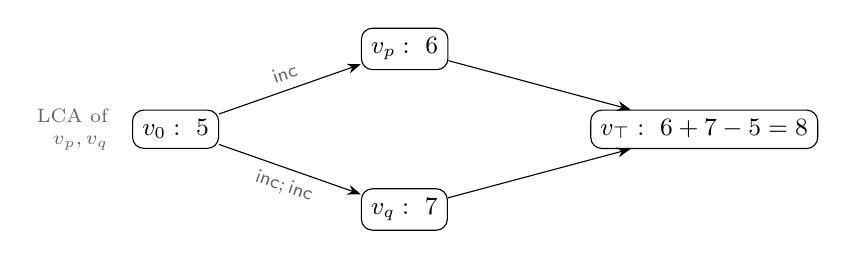
\begin{tikzpicture}[>=Stealth, node distance=0.75cm and 1.5cm,
  ver/.style={draw, rounded corners, inner sep=3.5pt, font=\small},
  lbl/.style={font=\scriptsize, text=black!60}]
\node[ver] (v0) {$v_0:\ 5$};
\node[ver, above right=0.5cm and 1.8cm of v0] (a1) {$v_p:\ 6$};
\node[ver, below right=0.5cm and 1.8cm of v0] (b1) {$v_q:\ 7$};
\node[ver, below right=0.5cm and 1.8cm of a1] (m) {$v_\top:\ 6+7-5 = 8$};
\draw[->] (v0) -- node[lbl, above, sloped]{$\mathsf{inc}$} (a1);
\draw[->] (v0) -- node[lbl, below, sloped]{$\mathsf{inc};\mathsf{inc}$} (b1);
\draw[->] (a1) -- (m);
\draw[->] (b1) -- (m);
\node[lbl, left=0.18cm of v0, align=right] {LCA of\\$v_p,v_q$};
\end{tikzpicture}
\caption{The counter MRDT. Both branches inherit the $5$ from the fork
point; the LCA argument lets the merge count each branch's \emph{delta}
exactly once. No binary merge of $6$ and $7$ alone can recover $8$: the
information ``how much is shared'' lives in the DAG, and the LCA argument
is how the data type reads it.}
\label{fig:counter}
\end{figure}

The Neem methodology (OOPSLA~2025) promises a clean division of labour:
the data-type designer discharges a fixed catalogue of equations over
$\mathsf{do}$, $\mergeL$ and the conflict-resolution relation
$\rcrel$ --- mostly by SMT --- and a soundness meta-theorem, proved
once, converts those VCs into \emph{RA-linearizability} of every reachable
configuration. This part documents what a Lean~4 mechanization of that
meta-theorem, in the full \textbf{ternary, version-DAG} setting, found:
the meta-theorem's central induction is unsound as written, and for
LCA-sensitive data types several of the catalogue's merge VCs are false
in principle when quantified over all states. It also develops the
corrected metatheory: a set-relative linearization order, canonical
states $\sigma(E)$ (each event set determines a unique state), and a
ternary \emph{Join Lemma} whose induction
consumes a small, contextual VC surface. Its contributions:

\begin{enumerate}[leftmargin=2em]
\item \textbf{The paper's LCA lemma is true but its proof has a gap}
  (\S\ref{sec:lca}): $L(v_\ell) = L(v_1) \cap L(v_2)$ holds, but only as a
  \emph{reachability invariant} of the store, whose proof needs a
  generator-uniqueness induction the paper silently assumes. We mechanize
  the transition system and the invariant.
\item \textbf{The soundness proof has a fully LCA-legal defeater}
  (\S\ref{sec:defeater}): a reachable configuration of a legal add-wins
  MRDT --- its final merge sitting at an honest LCA --- on which every
  bottom-up peel of the paper's derivation rules is stuck. The
  meta-theorem must be rebuilt, not patched.
\item \textbf{The lattice contract does not transfer; a delta contract does}
  (\S\ref{sec:whydelta}): the lattice laws are equations over \emph{free}
  tuples --- the wrong instances for an LCA-aware merge. Side-idempotence
  $\mergeL(l,a,a) = a$ with $l$ free fails for the counter ($2a-l$), but
  its only DAG-honest instance has $l = a$ (the LCA of a version with
  itself \emph{is} that version), where it holds trivially; and when two
  \emph{distinct} histories reach equal side states, $2a-l$ is the
  \emph{correct} merge --- both branches' increments count --- not an
  idempotence failure. The induced orders degenerate, and the honest
  associativity law has \emph{four distinct LCAs} and holds only on
  feasible tuples. The moral: the algebra of an LCA-aware merge is an
  algebra of \emph{causal histories}, not of concrete states. What
  replaces the lattice laws is a two-law \emph{delta contract} --- redistribution identities in which the LCA
  slot does, by arithmetic, the job idempotence does order-theoretically
  for CRDTs.
\item \textbf{Eight VCs suffice} (\S\ref{sec:vcs}--\S\ref{sec:adequacy}):
  three relational VCs on $\rcrel$ (one of them carrying a
  different-replica guard --- same-replica pairs are ordered by program
  order, and demanding $\rcrel$ cover them is unsatisfiable for
  real data types), merge symmetry, three
  feasibility-conditioned delta laws, and one contextual \emph{causal-delta}
  equation. The adequacy theorem is per \emph{version}: every version in
  the store, LCAs included, linearizes.
\item \textbf{The VC set is validated on the production catalogue}
  (\S\ref{sec:catalog}): the flat production MRDTs shipped in Sal ---
  OR-set, an optimized OR-set, enable-wins flag, grow-only set and map,
  increment-only and PN counters, a tombstone RGA, Peritext, the
  multi-valued register and the add-wins priority queue --- are
  discharged end-to-end, kernel-checked; the sequence data types with
  physical deletion go through the conditioned framework and its
  factored discharge route (\S\ref{sec:condmeta}--\S\ref{sec:route},
  Part~II). The sweep produces an empirical
  \emph{class map} of which data types need which strength of contract,
  with two surprises: tombstones are a metatheoretic trivializer, and
  commutativity class and delta class are independent axes.
\item \textbf{The metatheorem factors} (\S\ref{sec:route}): conditioning
  splits as a generic honest-reachability metatheorem times a
  per-datatype join discharge (\lean{HonestReach},
  \lean{JoinLemma3At}), with a uniform honesty shape (a client-checkable
  predicate holding of each event at the fold of its causal past). Three
  join species are observed in production (conditioned commutation, flat
  commutation, direct witness), and the mergeable queue, whose conflict
  graph admits no $\rcrel$ assignment at all, is the flagship of the
  direct-witness species: Peepul's merge is its own linearization
  certificate. The same route carries Part~II's embedded-chain RGA.
\end{enumerate}

Everything stated as a theorem below is mechanized with zero
\lean{sorry}s; \S\ref{sec:mech} maps statements to Lean names and files
(foundations under \lean{Framework/}, metatheorems under
\lean{Metatheory/}, negative results under \lean{Refutations/}, the
per-RDT instances under \lean{MRDT\_Instances/}, the investigation record
under \lean{Development/}; each cited theorem kernel-checked).


\section{Mergeable replicated data types, by definition and example}
\label{sec:mrdts}

\paragraph{Data type and implementation.} A replicated data type of
\emph{type} $\tau = \langle O_\tau, Q_\tau, \mathit{Val}_\tau\rangle$
exposes a set of update operations $O_\tau$, a set of query operations
$Q_\tau$, and a domain of query return values $\mathit{Val}_\tau$. An
\emph{MRDT implementation} of $\tau$ is a tuple
\[
  \M{D} \;=\; \langle \Sigma,\; \Sinit,\; \mathsf{do},\; \mergeL,\;
  \mathsf{query},\; \rcrel \rangle ,
\]
where $\Sigma$ is the space of replica states with initial state
$\Sinit$; $\mathsf{do} : \Sigma \times \M{E} \to \Sigma$ applies an
\emph{event} --- an update-operation instance $e = (t, r, o)$ carrying a
globally unique timestamp $t$, its origin replica $r$, and the operation
$o \in O_\tau$; $\mergeL : \Sigma^3 \to \Sigma$ is the three-way merge,
whose first argument is the state at the lowest common ancestor of the
two versions being merged; $\mathsf{query} : \Sigma \times Q_\tau \to
\mathit{Val}_\tau$ reads a state; and $\rcrel \subseteq O_\tau
\times O_\tau$ is the \emph{conflict-resolution} relation, consulted to
order concurrent non-commuting operations (it is the data-type designer's
declaration of who wins a race). Queries never change state and play no
role in the metatheory; the theory below reads the implementation as
$\langle \Sigma, \Sinit, \mathsf{do}, \mergeL, \rcrel\rangle$.

\paragraph{Describing an MRDT: the counter.} To describe an MRDT one
gives the five components and, when operations can race, says who wins.
The increment-only counter of Figure~\ref{fig:counter} is the smallest
complete example:
\[
  \Sigma = \mathbb{Z}, \qquad \Sinit = 0, \qquad
  \mathsf{do}(\sigma, (t,r,\mathsf{inc})) = \sigma + 1, \qquad
  \mergeL(l,a,b) = a + b - l, \qquad \rcrel = \emptyset .
\]
All operations commute, so $\rcrel$ is empty --- yet the merge
genuinely uses its LCA argument: $a + b$ alone would double-count the
history shared by the two branches, and the $-\,l$ subtracts it exactly
once. This ``read the shared past off the LCA'' pattern recurs
throughout the catalogue.

\paragraph{A data type with races: the OR-set.} The add-wins observed-remove
set stores tagged elements: $\add$ inserts a tag unique to the adding
event, $\rem$ deletes exactly the tags it has \emph{seen}. Sequentially,
a remove after an add deletes it; concurrently the designer declares the
add the winner: $\rem \rc \add$. The merge keeps a tag iff both sides
have it (nobody deleted it) or some side added it since the fork:
\[
  \mergeL(l,a,b) \;=\; (a \cap b) \cup (a \setminus l) \cup (b \setminus l).
\]
The LCA here plays the role a tombstone set plays for the CRDT OR-set:
deletion is absence \emph{relative to} $l$, and the state needs no
graveyard.

\paragraph{The generalized signature.} Both examples' operations make
sense on \emph{every} state: any state can be incremented, any tag can be
added. Such data types are \emph{flat}, and for them the metatheory of
\S\ref{sec:setting}--\S\ref{sec:catalog} quantifies its VCs over all
states. But a data type whose operations carry \emph{preconditions} ---
insert under a node that must exist, delete a node that must be live ---
breaks that quantification: its commutation equations are simply false at
nonsense states. The full signature therefore extends the tuple with
three declarations (\lean{ConditionedMRDTSig}; formalized in
\S\ref{sec:cvcs}):
\[
  \M{D} \;=\; \langle \Sigma, \Sinit, \mathsf{do}, \mergeL, \rcrel,\;
  \Inv,\; \app \rangle
  \quad\text{together with}\quad {\eqobs} \subseteq \Sigma \times \Sigma ,
\]
where $\Inv$ is a state invariant (a shape over-approximation of
reachability), $\app$ an applicability predicate (when an event is
sensible at a state), and $\eqobs$ an observational equivalence (what
queries can distinguish; representation residue is quotiented away).
Commutation is then required only at $\Inv$-states where both events are
applicable. Flat data types take $\Inv = \app = \top$ and
${\eqobs} = {=}$, collapsing the general signature to the plain one ---
one framework, of which \S\ref{sec:setting}--\S\ref{sec:catalog} is the
flat instance and \S\ref{sec:condmeta} onwards the general case.

\paragraph{The running hard example: sequences with physical deletion.}
The datatype class that forces the general signature is the replicated
list underlying collaborative text editing. Characters are nodes
identified by timestamps, each inserted \emph{after} an anchor node;
production RGAs keep deleted nodes as \emph{tombstones} because later
concurrent inserts may still anchor on them, and a \emph{tombstone-free}
design deletes physically. Its operations are precondition-laden: an
insert names an anchor that must exist, a delete names a live node, and
the flat update layer quantifies its commutation VCs over every state,
including nonsense states no execution produces, where those equations
are false. Worse, what makes reachable-state commutation true is a
property of the \emph{execution that generated the operation} (the
issuer saw the anchor live), not of the state the operation later meets,
so it is not expressible as a $\forall\sigma$ equation over the
signature alone. This is the reason the general signature exists: $\Inv$
and $\app$ name the sensible states and operations, an honesty
discipline makes generation-time facts available to the proofs, and
$\eqobs$ absorbs representation residue. Part~II presents the
embedded-chain RGA, the sequence datatype that holds the repository's
canonical seat, together with its end-to-end discharge through the
factored route of \S\ref{sec:route}; a predecessor design that carried
recorded ancestor paths and rehomed orphans on delete was proved
RA-linearizable in the same framework and was later demoted by its
sequential refutation (Part~III).

\section{The ternary setting}
\label{sec:setting}

This section fixes the model: the data-type signature, the replicated
store and its transitions, and the specification the metatheorem must
deliver. The definitions are the paper's, with one correction flagged
where it occurs.

\paragraph{Signature.} An MRDT is $\langle \Sigma, \Sinit, \mathsf{do},
\mergeL, \rcrel\rangle$ as in \S\ref{sec:mrdts}, read flat for now
($\Inv = \app = \top$, ${\eqobs} = {=}$; the general case resumes in
\S\ref{sec:condmeta}). We write $e(\sigma)$ for
$\mathsf{do}(\sigma,e)$, and $e_1 \comm e_2$ when
$e_1(e_2(\sigma)) = e_2(e_1(\sigma))$ for every $\sigma$.

\paragraph{Executions.} A configuration carries a \emph{store}: a DAG of
versions, each holding a state and the set of events that produced it,
with per-replica heads. Transitions fork a replica, apply a fresh event at
a head, query, or \textbf{merge}: pick heads $v_1, v_2$, find their LCA
$v_\ell$ in the DAG, and install a new version with state
$\mergeL(\sigma_{v_\ell}, \sigma_{v_1}, \sigma_{v_2})$ and event set
$L(v_1) \cup L(v_2)$. Visibility $\vis$ records what each event's issuing
replica had seen.

\paragraph{RA-linearizability, per version.} Write $e_1 \parallel e_2$
when neither $e_1 \vis e_2$ nor $e_2 \vis e_1$ (concurrency).

\begin{definition}[linearization order, set-relative]
\label{def:lo}
For an event set $E$, the order $\loE{E}$ puts $e_1$ before $e_2$ iff
\[
\bigl(e_1 \vis e_2 \;\wedge\; e_1 \ncomm e_2\bigr)
\;\;\vee\;\;
\bigl(e_1 \parallel e_2 \;\wedge\; e_1 \rc e_2 \;\wedge\;
  \neg\,\exists e_3 \in E.\;\; e_2 \vis e_3 \,\wedge\, e_2 \ncomm e_3\bigr):
\]
a visible non-commuting pair is ordered by visibility; a concurrent pair
whose conflict $\rcrel$ resolves is ordered by $\rcrel$ ---
unless $e_2$ is already \emph{absorbed} (overwritten) by a later
non-commuting event of $E$. The paper's order $\mathsf{lo}$ is the
variant whose absorber clause ranges over the whole configuration; since
a $\mathsf{lo}$-edge asserts \emph{no absorber anywhere},
$\mathsf{lo} \subseteq \loE{E}$ pointwise, for every $E$.
\end{definition}

\begin{definition}[RA-linearizability]
\label{def:ralin}
A list $\pi = e^1 e^2 \cdots e^n$ \emph{witnesses} a version holding
state $s$ and event set $E$ when (i)~$\pi$ enumerates $E$ without
repetition; (ii)~$\pi$ \emph{extends} $\mathsf{lo}$: $i < j$ implies
$\neg(e^j \mathrel{\mathsf{lo}} e^i)$; and (iii)~$\pi$ \emph{folds} to
the state: $e^n(\cdots e^2(e^1(\Sinit))\cdots) = s$. A configuration is
\emph{RA-linearizable} when \emph{every version in the store} --- not
only the replica heads; LCAs are historical versions and the merge reads
them --- admits a witness. In the general signature the fold clause
(iii) is read up to the data type's observational equivalence,
$e^n(\cdots e^1(\Sinit)\cdots) \eqobs s$ --- the same definition with
its equality parameter generalized; flat data types instantiate
${\eqobs} = {=}$ and this section's form is exactly that instance.
\hfill\lean{IsRALinearizable3}, \lean{IsRALinearizable3Eq}
\end{definition}

Why a set-relative order? One definitional correction is forced at the
outset: for every internal use, the absorber clause must range over the
event set of \emph{the version being linearized}, not over the whole
configuration --- an event can gain absorbers from another branch,
silently cancelling an order edge inside a version whose own state
depends on it (the defeater of \S\ref{sec:defeater} realizes exactly
this). We therefore construct witnesses respecting $\loE{E}$ throughout;
since $\mathsf{lo} \subseteq \loE{E}$, every such witness also extends
the paper's order, and Definition~\ref{def:ralin} is delivered exactly
as the paper states it.

\paragraph{Running examples.} Three data types exercise every corner of
the theory:
\begin{itemize}[leftmargin=2em]
\item the \textbf{counter}: $\Sigma = \mathbb{Z}$,
  $\mathsf{inc}(\sigma) = \sigma+1$, $\mergeL(l,a,b) = a+b-l$; all
  operations commute, but the merge genuinely uses its LCA;
\item the \textbf{OR-set} (tagged add-wins set): elements are tagged by
  the adding event's timestamp; $\rem$ deletes the tags it has seen;
  concurrently, $\rem \rc \add$ resolves in favour of the add. The merge
  keeps an element iff \emph{both} sides have it or \emph{some} side added
  it since the fork:
  \[
    \mergeL(l,a,b) \;=\; (a \cap b) \,\cup\, (a \setminus l) \,\cup\, (b
    \setminus l)
  \]
  --- pointwise, ``if the tag is in $l$, require it in both branches
  (nobody deleted it); otherwise one branch suffices (somebody added
  it).'' Here the LCA acts as a \emph{tombstone set}: deletion is
  represented by \emph{absence relative to} $l$, so the state itself needs
  no graveyard;
\item the \textbf{enable-wins flag}: per-replica pairs
  $(\text{counter},\text{flag})$; enabling bumps your own counter and sets
  your flag; disabling clears all flags; the merge compares each
  replica's counter against the LCA's to decide whether an enable
  ``happened since the fork'' on that replica. Its merge \emph{compares}
  counters rather than accumulating sets --- and that difference will be
  visible in the metatheory (\S\ref{sec:catalog}).
\end{itemize}

\section{Three facts the metatheory must respect}

Before building anything, we record two boundary facts about the
paper's development: its store-level LCA lemma is true but under-proved,
and its soundness induction is refuted by a fully legal execution.
Together they fix the shape of the corrected metatheory --- resting on a
mechanized store invariant (\S\ref{sec:lca}) and built around the join
rather than the sides (\S\ref{sec:defeater}).

\subsection{The LCA lemma is a reachability invariant --- with a gap in the
published proof}
\label{sec:lca}

Everything above silently used:

\begin{lemma}[LCA lemma]
\label{lem:lca}
In every reachable configuration, if $v_\ell$ is an LCA of versions $v_1,
v_2$ in the store's DAG, then $L(v_\ell) = L(v_1) \cap L(v_2)$.
\end{lemma}

This is what lets merge VCs be stated over \emph{event sets}: the state
the merge receives as $l$ is the canonical state of exactly the
intersection of the two sides' histories. The lemma is true --- but it is
a \emph{global induction over the reachable store}, not a local fact. Its
mechanized proof threads a store invariant (all parents allocated; event
sets monotone along edges; and an \emph{origin} invariant --- each event
appears first at a unique generator version) through every transition; the
published proof asserts the generator-uniqueness step without the
induction that sustains it. An erratum-sized gap: the statement survives,
the proof as written does not. (A related boundary fact:
\emph{criss-cross} merges can defeat the \emph{existence} of an
LCA --- they gate merge-enabledness, not the lemma. Open
Question~\ref{oq:crisscross} takes up the extension.)

\subsection{A fully LCA-legal execution defeats the soundness proof}
\label{sec:defeater}

The generic half of the paper's contract is a \emph{bottom-up
linearization} theorem: given linearization witnesses for the two sides
of a merge, construct one for the merged version by repeatedly
\emph{peeling} a final event through $\mergeL$ using the catalogue's
interchange VCs. One might hope the version DAG's discipline --- every
merge sitting at an honest LCA --- keeps the peel supplied with peelable
events. It does not: one staging replica suffices to realize the
intersection of two histories as an honest version, and the merge
induction is stuck.

\begin{example}[the defeater]
\label{ex:defeater}
The data type is a one-key add-wins skeleton with tagged adds:
$\sigma = (A, D) \in 2^{\mathbb{T}} \times 2^{\mathbb{T}}$ with live set
$A \setminus D$; $\add_t$ inserts its tag into $A$; $\rem$ kills
everything it currently sees ($D \coloneqq A \cup D$ --- the
state-dependence is what makes $\add \ncomm \rem$); concurrently
$\rem \rc \add$ (add wins); the merge is componentwise union, ignoring
its LCA argument. A legal MRDT.
Replica $p$ adds ($A_p$), replica $q$ adds ($A_q$). A staging replica $s$
merges both one-add versions, creating $v_s$ with
$L(v_s) = \{A_p, A_q\}$. Now $p$ removes ($R_p$, seeing only $A_p$) and
then merges with $v_s$; symmetrically $q$ removes ($R_q$) and merges with
$v_s$. Figure~\ref{fig:defeater} shows the DAG. The final merge of the two
heads finds $\mathrm{LCA} = v_s$, and
$L(v_s) = \{A_p,A_q\} = L(\text{head}_p) \cap L(\text{head}_q)$ --- the
configuration is fully legal. Now count last events. $p$'s head lives on
exactly $A_q$'s tag, so a state-correct witness must run $R_p$ before
$A_q$, and neither $R_p$ nor $A_p$ can come last: every linearization of
$p$'s head ends in $A_q$. Symmetrically, every linearization of $q$'s
head ends in $A_p$. Yet in the \emph{merged} version every tag is dead,
so its linearizations must end in one of the removes.
The events the induction must peel are \emph{buried} in the very sides
that own them; no ordering of the paper's bottom-up rules applies.
\end{example}

The two removes commute ($\rem \ncomm \add$ but $\rem \comm \rem$), which
invites a particular rescue attempt: the paper's \textsc{BottomUp-2-OP}
rule (\lean{inter\_lca\_2op}) admits the commuting case and could, one
hopes, peel a remove last. It cannot, for a reason that is a one-line
state fact. To peel $o$ last from a side, that side's state must be an
$o$-image --- of the form $\mathsf{do}(\sigma', o)$ with $o$ outermost.
But in the add-wins skeleton \emph{every} $\rem$-output has empty live set
($\rem(A,D) = (A, A\cup D)$), whereas both heads carry a live tag
($\mathrm{head}_p$ lives on $A_q$, $\mathrm{head}_q$ on $A_p$ --- the
opposite add, merged in \emph{after} the local remove). So neither head
is a $\rem$-image, and no bottom-up rule can extract a remove from it. The
tempting linearization $[A_p, R_p, A_q, R_q]$ is a valid witness of the
\emph{merged} version, but its restriction to $\mathrm{head}_q$ folds to
the all-dead state, not $\mathrm{head}_q$'s actual state (live $A_p$): it
is not assembled from a state-correct side witness, which is exactly what
the induction requires. All three facts are mechanized
(\lean{InterLca2op\_Defeater\_Arbiter}: \lean{awset\_rem\_output\_empty},
\lean{no\_inter\_lca\_2op\_rem\_peel\_of\_defeater}, \lean{crack1\_witness}).

\begin{figure}[t]
\centering
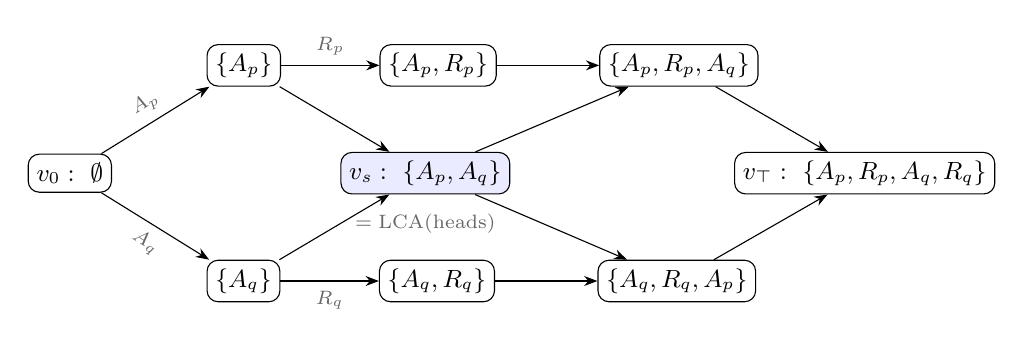
\begin{tikzpicture}[>=Stealth, node distance=0.55cm and 1.35cm,
  ver/.style={draw, rounded corners, inner sep=3pt, font=\small},
  lca/.style={draw, rounded corners, inner sep=3pt, font=\small,
    fill=blue!8},
  lbl/.style={font=\scriptsize, text=black!60}]
\node[ver] (v0) {$v_0:\ \emptyset$};
\node[ver, above right=0.85cm and 1.2cm of v0] (p1) {$\{A_p\}$};
\node[ver, below right=0.85cm and 1.2cm of v0] (q1) {$\{A_q\}$};
\node[lca, right=2.9cm of v0] (s) {$v_s:\ \{A_p,A_q\}$};
\node[ver, right=1.25cm of p1] (p2) {$\{A_p,R_p\}$};
\node[ver, right=1.25cm of q1] (q2) {$\{A_q,R_q\}$};
\node[ver, right=1.3cm of p2] (p3) {$\{A_p,R_p,A_q\}$};
\node[ver, right=1.3cm of q2] (q3) {$\{A_q,R_q,A_p\}$};
\node[ver, right=7.9cm of v0] (top) {$v_\top:\ \{A_p,R_p,A_q,R_q\}$};
\draw[->] (v0) -- node[lbl, above, sloped]{$A_p$} (p1);
\draw[->] (v0) -- node[lbl, below, sloped]{$A_q$} (q1);
\draw[->] (p1) -- (s);
\draw[->] (q1) -- (s);
\draw[->] (p1) -- node[lbl, above]{$R_p$} (p2);
\draw[->] (q1) -- node[lbl, below]{$R_q$} (q2);
\draw[->] (p2) -- (p3);
\draw[->] (s) -- (p3);
\draw[->] (q2) -- (q3);
\draw[->] (s) -- (q3);
\draw[->] (p3) -- (top);
\draw[->] (q3) -- (top);
\node[lbl, below=0.12cm of s] {$=\mathrm{LCA}(\text{heads})$};
\end{tikzpicture}
\caption{The defeater (Example~\ref{ex:defeater}). Nodes are
versions labelled by their event sets; the shaded version $v_s$, created
by a staging replica, realizes $L(\text{head}_p)\cap L(\text{head}_q)$ as
an honest store version, so the final merge is LCA-legal. The removes
$R_p, R_q$ --- the only events a bottom-up derivation may peel last ---
are buried mid-history on their own sides.}
\label{fig:defeater}
\end{figure}

The consequence for the design: the metatheorem cannot be patched
peel-by-peel --- it must be rebuilt on canonical states and a Join Lemma,
with merge-side VCs that are statements \emph{about the join}, not about
how either side's state factors.

\section{Canonical states and the ternary Join Lemma}
\label{sec:join}

We now rebuild --- new proof architecture, and with it a \emph{new set
of verification conditions} to replace the paper's catalogue. The lesson
of the defeater is architectural: witnesses for a merged version cannot
be manufactured out of witnesses for its sides, so the corrected
metatheory must not traffic in witness lists at all. The rebuild has two
layers. The \emph{update layer} makes states, not sequences, the objects
of the induction: it assigns to every event set $E$ a single
well-defined state, its \emph{canonical state}
(Definition~\ref{def:sigma} below). The \emph{merge layer} is then one
equation between canonical states --- the ternary \emph{Join Lemma} ---
and establishing it from per-data-type VCs becomes the entire burden of
the metatheorem (\S\ref{sec:whydelta}--\S\ref{sec:vcs}).

The update layer comes first, and a structural observation makes it
cheap: this half of the corrected theory never mentions the merge. Its
one theorem is stated over the update signature $\langle \Sigma, \Sinit,
\mathsf{do}, \rcrel\rangle$ alone:

\begin{theorem}[convergence]
\label{thm:conv}
Assume the update-layer VCs (items 1--3 of \S\ref{sec:vcs}). Then any
two $\loE{E}$-respecting enumerations of a finite event set $E$ fold
from $\Sinit$ to the same state.
\end{theorem}

This is where the set-relative reading of \S\ref{sec:setting} earns
its keep: with the paper's configuration-wide order in place of
$\loE{E}$, the theorem is \emph{false} --- the defeater's heads are
already counterexamples, since two order-respecting replays of the
three events of $\mathrm{head}_p$ reach different states. Convergence
licenses a definition:

\begin{definition}[canonical state]
\label{def:sigma}
For a finite event set $E$, the \emph{canonical state} $\sigma(E)$ is
the state obtained by folding any $\loE{E}$-respecting enumeration of
$E$ from $\Sinit$. At least one respecting enumeration exists because
$\loE{E}$ is acyclic (VC~2); the result is independent of the choice by
Theorem~\ref{thm:conv}; and $\sigma(\emptyset) = \Sinit$. We write
$\sigma(E)$ for the canonical state of an event set, and $\sigma_v$ for
the state a version $v$ happens to hold in the store --- proving that
the two coincide is precisely the metatheorem's job.
\end{definition}

With canonical states in hand, witness lists disappear as promised: a
version linearizes iff $\sigma_v = \sigma(L(v))$ --- the witness, when
one is owed, is any respecting enumeration of $L(v)$. The induction can
therefore maintain a state-level invariant (``every version holds
$\sigma$ of its events'') instead of constructing sequences. The one
genuinely ternary statement is what the merge must produce:

\begin{definition}[ternary Join Lemma]
For backward-closed event sets $E_1, E_2$ of a reachable configuration,
\[
  \sigma(E_1 \cup E_2)
  \;=\;
  \mergeL\bigl(\sigma(E_1 \cap E_2),\; \sigma(E_1),\; \sigma(E_2)\bigr).
\]
\end{definition}

By Lemma~\ref{lem:lca} the first argument is exactly the state the store
hands the merge. The adequacy proof (\S\ref{sec:adequacy}) is then an
induction over the transition system maintaining ``every version holds the
canonical state of its event set''; the merge case \emph{is} the Join
Lemma. What remains is the question this part exists to answer: which
per-data-type VCs make the Join Lemma true?

\section{Why the contract is a delta contract}
\label{sec:whydelta}

Where should the laws that prove the Join Lemma come from? The obvious
supplier is the CRDT tradition. For state-based CRDTs --- binary merge,
no LCA --- merge-coherence is lattice-flavoured: associativity,
idempotence, inflation of updates. None of the three transfers to the
ternary merge: their free-tuple forms are the wrong equations for an
LCA-aware merge, and their honest instances are too weak to power a
lattice-style proof. This section works through why, because the shape
of what fails to transfer reveals the contract that succeeds.

\paragraph{Idempotence: the free-tuple form is the wrong equation.}
The \emph{diagonal} law $\mergeL(a,a,a) = a$ --- the paper's own
\textsc{MergeIdempotence} --- holds (for the counter: $a + a - a = a$),
but it is not the law a lattice-style proof consumes. The binary
architecture uses idempotence to absorb a duplicated \emph{side},
$\Merge(a,a) = a$, with nothing tying the two copies to a common past;
the ternary analogue would be $\mergeL(l,a,a) = a$ with $l$ \emph{free}.
But quantifying $l$ freely asks the merge about tuples the version DAG
never produces. Merging a version with \emph{itself} has $l = a$ --- the
LCA of $a$ and $a$ is $a$ --- where the law collapses to the diagonal
and holds. And when two \emph{distinct} histories happen to reach equal
side states, feasibility puts $l$ strictly below them and the counter's
$\mergeL(l,a,a) = 2a - l$ is the \emph{correct} answer: both branches'
increments count. So there is no idempotence \emph{failure} --- there is
no meaningful side-idempotence \emph{law}: its honest instances are the
trivial diagonal, and demanding it unconditionally would exclude
precisely the LCA-sensitive data types the ternary theorem exists for.

The general principle, which the rest of this section instantiates: the
algebraic properties of an LCA-aware merge are properties of the
\emph{causal history}, not of the concrete state. Two sides merge
idempotently when their \emph{histories} coincide --- which is what
forces $l = a$ --- not when their states happen to be equal; equal
states with different histories rightly merge differently. The lattice
laws go wrong exactly by quantifying over states while forgetting the
histories that produced them, and every law that survives below is
stated over history-indexed data: canonical states $\sigma(E)$, feasible
tuples (the LCA slot carrying the intersection history), downset deltas.

\paragraph{No usable order.} The lattice-style workhorse order
$x \sqsubseteq y \coloneqq \Merge(x,y) = y$ has ternary candidates
$x \sqsubseteq_l y \coloneqq \mergeL(l,x,y) = y$, but for the counter this
relation degenerates to $x = l$; no antisymmetry survives to power
order-theoretic reasoning. The single
contextual VC below is accordingly an \emph{equation}, not an inequality.

\paragraph{Associativity is the wrong target.} The natural guess ---
$\mergeL(l,\mergeL(l,a,b),c) = \mergeL(l,a,\mergeL(l,b,c))$ --- assumes
one LCA for all three merges. In an execution, re-associating a three-way
reconciliation involves \emph{four} distinct LCAs:
\[
  \mergeL\bigl(l_{(ab)c},\, \mergeL(l_{ab}, a, b),\, c\bigr)
  \;\overset{?}{=}\;
  \mergeL\bigl(l_{a(bc)},\, a,\, \mergeL(l_{bc}, b, c)\bigr),
\]
with $l_{ab} = \sigma(E_a \cap E_b)$, $l_{(ab)c} = \sigma((E_a \cup E_b)
\cap E_c)$, and so on. For the counter --- whose canonical states are
additive measures over event sets --- the two sides come to $a+b+c$ minus
the two LCA measures, and they agree because
\[
  (E_a \cup E_b) \cap E_c = (E_a \cap E_c) \cup (E_b \cap E_c)
  \quad\Longrightarrow\quad
  \text{both LCA-sums} = |E_{ab}| + |E_{ac}| + |E_{bc}| - |E_{abc}|
\]
by inclusion--exclusion. The law holds, but only \emph{through the
set-algebra of intersections}: over four unconstrained states it is false.
Honest associativity is inherently a feasible-tuple fact --- and, the
mechanization's pleasant surprise, \textbf{the corrected induction never
needs it}. Every merge the induction forms already sits at its honest LCA;
the only laws consumed are two \emph{redistribution} identities that
equate two honestly-formed merges:

\begin{definition}[the delta contract]
\label{def:delta}
\begin{align*}
\textsc{local-redistribute}:&\quad
  \mergeL(l,\, \mergeL(m, x, c),\, y) \;=\; \mergeL(m,\, \mergeL(l, x,
  y),\, c),\\
\textsc{redistribute}:&\quad
  \mergeL\bigl(\mergeL(m,x_0,c),\, \mergeL(m,x_1,c),\, \mergeL(m,x_2,c)\bigr)\\
  &\qquad\qquad\qquad\;=\; \mergeL\bigl(m,\, \mergeL(x_0,x_1,x_2),\, c\bigr).
\end{align*}
\end{definition}

Read $c$ as a \emph{delta relative to $m$} (in the induction, $c$ will be
``apply event $e$ to its causal past''). \textsc{local-redistribute} says
a delta application commutes past an enclosing merge through one branch
slot. \textsc{redistribute} says a delta carried by \emph{all three}
components extracts \emph{once} --- the LCA slot cancels the duplicates by
arithmetic. This is the delta contract's quiet coup: cancelling the
duplicated shared contribution is exactly the job idempotence performs in
lattice-based convergence arguments, now done without any idempotence ---
which is why the
counter sails through ($\textsc{redistribute}$ for the counter is the
identity $\sum x_i + 3c - 3m - (x_0 + c - m) - \cdots$ collapsing on both
sides).

\paragraph{Where the contract holds unconditionally --- and where it
cannot.} The two laws hold \emph{on all states} exactly for the
group-like class (the counter) and the lattice-like, LCA-blind class
(grow-only structures). They are \emph{unconditionally false} for the
OR-set: take an element tag present in $c$ and $l$ but in neither branch
--- the two sides of \textsc{local-redistribute} then disagree about
whether the LCA's copy survives. But such a tuple can never arise: a tag
in a canonical LCA state is in \emph{both} branches unless removed, and a
removal is itself an event of the branch. The failing tuples are
\emph{infeasible}, and this is a theorem-grade phenomenon, not an
inconvenience:

\begin{finding}
For LCA-sensitive MRDTs beyond the group $\oplus$ lattice classes, the
merge-coherence laws are irreducibly \emph{feasibility-conditioned}: true
on canonical tuples at honest LCAs, false in general. Quantifying merge
VCs over all states --- the published catalogue's style --- is not merely
inconvenient for such data types; for several laws it is wrong in
principle. (The enable-wins flag even falsifies the \emph{unit} law
$\mergeL(\Sinit,\Sinit,s)=s$ on an infeasible state with a set flag and a
zero counter.)
\end{finding}

Accordingly the delta laws enter the final contract in
feasibility-conditioned form: quantified over canonical states of
backward-closed event sets, with every $\mergeL$ node at its honest LCA.
The unconditional form remains available as a one-line \emph{on-ramp} (it
trivially implies the conditioned form) for the group and lattice
classes.

\section{The eight verification conditions}
\label{sec:vcs}

\begin{figure}[t]
\centering
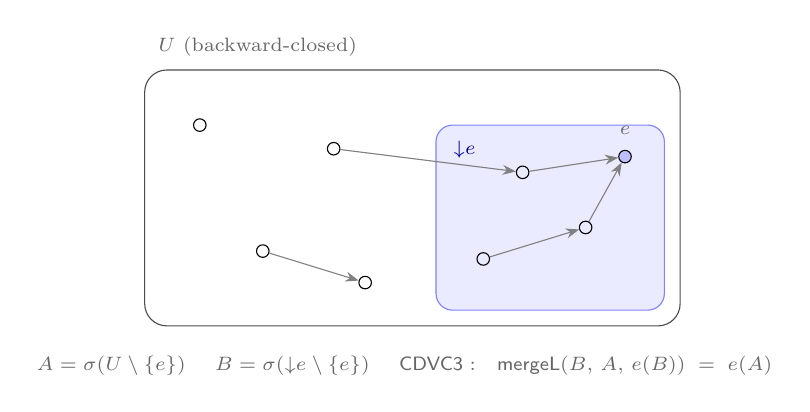
\begin{tikzpicture}[>=Stealth,
  ev/.style={circle, draw, inner sep=1.6pt, font=\scriptsize},
  lbl/.style={font=\scriptsize, text=black!60}]
% the big set U
\draw[rounded corners=8pt, black!70]
  (-0.4,-0.35) rectangle (6.4,2.9);
\node[lbl, anchor=south west] at (-0.35,2.95) {$U$ (backward-closed)};
% downset region
\begin{scope}[on background layer]
\fill[blue!8, rounded corners=6pt] (3.3,-0.15) rectangle (6.2,2.2);
\end{scope}
\draw[rounded corners=6pt, blue!50] (3.3,-0.15) rectangle (6.2,2.2);
\node[lbl, text=blue!60!black, anchor=north west] at (3.4,2.12) {$\dow{e}$};
% events
\node[ev] (x1) at (0.3,2.2) {};
\node[ev] (x2) at (1.1,0.6) {};
\node[ev] (x3) at (2.0,1.9) {};
\node[ev] (x4) at (2.4,0.2) {};
\node[ev] (y1) at (3.9,0.5) {};
\node[ev] (y2) at (4.4,1.6) {};
\node[ev] (y3) at (5.2,0.9) {};
\node[ev, fill=blue!25] (e) at (5.7,1.8) {};
\node[lbl, above=0.07cm of e] {$e$};
\draw[->, black!50] (y1) -- (y3);
\draw[->, black!50] (y2) -- (e);
\draw[->, black!50] (y3) -- (e);
\draw[->, black!50] (x3) -- (y2);
\draw[->, black!50] (x2) -- (x4);
\node[lbl] at (2.9,-0.85)
  {$A = \sigma(U\setminus\{e\})$ \quad
   $B = \sigma(\dow{e}\setminus\{e\})$ \quad
   $\cd:\ \ \mergeL(B,\, A,\, e(B)) \;=\; e(A)$};
\end{tikzpicture}
\caption{The causal-delta equation. The shaded region is $e$'s causal
past $\dow{e}$ (what $e$ saw); $e$ is $\loE{U}$-maximal. $e$'s effect on
the whole world $A$ equals: compute $e$'s effect on its own causal past
$B$, then merge that delta into $A$ \emph{over LCA $B$}. The merge sits at
its honest LCA: $(U\setminus\{e\}) \cap \dow{e} =
\dow{e}\setminus\{e\}$. Concurrent context that $e$ never observed
cannot amplify what $e$ does.}
\label{fig:cd}
\end{figure}

The update-side obligations of \S\ref{sec:join} and the merge-side laws
of \S\ref{sec:whydelta} now assemble into the full contract --- a
\emph{new} VC set, replacing the paper's catalogue of twenty-four. For
an MRDT $\langle \Sigma, \Sinit, \mathsf{do}, \mergeL,
\rcrel\rangle$, the contract is:

\paragraph{Update layer (unconditional, SMT-shaped).}
\begin{enumerate}[leftmargin=2.2em]
\item \textbf{rc-non-comm (guarded)} --- for distinct events \emph{from
  different replicas}: they fail to commute iff $\rcrel$ orders them
  in exactly one direction. \emph{The conflict table is the commutativity
  table, with a direction.} The different-replica guard is a semantic
  necessity, not a convenience: same-replica events are totally ordered
  by program order, so they are never concurrent and there is no
  conflict for $\rcrel$ to resolve. An unguarded VC would instead
  demand that $\rcrel$ order \emph{every} non-commuting pair ---
  unsatisfiable for real data types: the \emph{optimized OR-set}'s
  same-replica same-element adds do not commute (the newer add evicts
  the older tag), yet they can never race, and its $\rcrel$
  rightly ignores them. (The paper's F\textsuperscript{*} artifact
  carries exactly this guard in its interface ---
  \lean{App\_mrdt.fsti}: \texttt{requires distinct\_ops o1 o2
  /\char`\\\ get\_rid o1 <> get\_rid o2}.)
\item \textbf{no-rc-chain} --- conflict priorities do not chain: never
  $o_1 \rc o_2$ and $o_2 \rc o_3$. This is what makes the linearization
  order acyclic, so maximal events exist --- the entire peel-and-recurse
  architecture stands on it.
\item \textbf{cond-comm} --- a resolved conflict is invisible once an
  absorber runs: swapping an $\rcrel$-ordered concurrent pair deep in
  a fold changes nothing for any later non-commuting event, across
  arbitrary intervening events. This is the engine of convergence.
\end{enumerate}

\paragraph{Merge layer.}
\begin{enumerate}[leftmargin=2.2em]\setcounter{enumi}{3}
\item \textbf{merge symmetry} --- $\mergeL(l,a,b) = \mergeL(l,b,a)$.
\item \textbf{feasible unit} --- $\mergeL(\Sinit,\Sinit,\sigma(E)) =
  \sigma(E)$: merging over nothing is a no-op, on states that can arise.
\item \textbf{feasible local-redistribute} and
\item \textbf{feasible redistribute} --- Definition~\ref{def:delta},
  quantified over canonical tuples at honest LCAs.
\item \textbf{the causal-delta equation ($\cd$)} --- for a
  $\loE{U}$-maximal event $e$ of a backward-closed $U$, with
  $A = \sigma(U\setminus\{e\})$ and $B = \sigma(\dow{e}\setminus\{e\})$
  the canonical state of $e$'s own causal past:
  \[
    \mergeL\bigl(B,\; A,\; e(B)\bigr) \;=\; e(A).
  \]
  \emph{What an event does is determined by what it saw}
  (Figure~\ref{fig:cd}): applying $e$ to the whole world equals computing
  $e$'s delta on its causal past and merging it in over that past.
\end{enumerate}

Items 1--4 are one-liners for every data type we have discharged; items
6--7 frequently hold unconditionally anyway (for the OR-set,
\textsc{redistribute} is a pointwise Boolean tautology); essentially the
entire per-data-type proof effort concentrates in item 8, whose discharge
follows a uniform recipe: characterize $\sigma(E)$ (a ``sandwich''
invariant along canonical enumerations), then a \emph{trichotomy} placing
every event the maximal $e$ interacts with either inside $\dow{e}$ or
absorbed on a side that owns it.

Compare the published catalogue: 24~VCs per data type, plus five more the
soundness proof uses silently. Seventeen of the~24 --- the
\textsc{BottomUp} induction-scheme families --- exist to drive the broken
induction and are consumed nowhere in the corrected one; the paper's
\textsc{MergeIdempotence} is likewise never used. The seventeen were,
however, doing honest work of a different kind: they are an
\emph{automation layer}, Skolemizing ``holds on feasible states'' into
base-and-step equations an SMT solver can discharge. Rebuilding that
layer, aimed at the corrected target ($\cd$ rather than \textsc{BottomUp}),
is in our view the most valuable open engineering problem this work
leaves (\S\ref{sec:open}).

\section{Adequacy}
\label{sec:adequacy}

The contract delivers. Everything a data type owes is the eight
equations of \S\ref{sec:vcs}; everything else is proved once, for all
data types, as part of the execution model.

\begin{theorem}[soundness of the eight VCs]
\label{thm:main}
If an MRDT satisfies VCs 1--8, then every configuration reachable from
the initial configuration in the ternary transition system is
RA-linearizable, per version.
\hfill\lean{ra\_linearizable\_of\_core\_feasible\_cd3}
\end{theorem}

The proof shape: the update layer powers the set-relative convergence
theorem, hence canonical states; the transition induction maintains
``every store version is canonical for its event set'' (fork and query
are trivial; apply is the extend lemma); the merge case reduces, via
Lemma~\ref{lem:lca}, to the ternary Join Lemma, which is proved from VCs
4--8 by strong induction on $|E_1 \cup E_2|$: select a
$\loE{E_1\cup E_2}$-maximal $e$, decompose each side containing $e$
through $\dow{e}$ (\textsc{local-redistribute} at the honest LCA
$\dow{e}\setminus\{e\}$), cancel the shared delta
(\textsc{redistribute}), close the principal step with $\cd$, and recurse.
The buried-event pathology of Example~\ref{ex:defeater} dissolves
structurally: no step ever asks how a \emph{side's} state factors ---
every factoring happens through the join.

Everything else one might fear owing is proved once, for all data types,
as an execution-model invariant: visibility transitivity, per-version
backward closure, store well-formedness, and Lemma~\ref{lem:lca} itself.
The data type owes exactly the eight equations.

\paragraph{A second route, and an honest asymmetry.} One discharged data
type does not fit the pattern above. The enable-wins flag's merge
\emph{compares counters} against the LCA, and for such merges the Join
Lemma's hypotheses as stated (backward closure under
non-commuting-visibility) are provably too weak: there is a
closure-legal tuple --- a live LCA enable, a dead post-LCA enable
inflating one side's counter, the killing disable visible only to the
other side --- on which the production merge computes the wrong flag. Full
\emph{causal} closure (which the store invariant actually supplies)
excludes it, and the flag is discharged through a full-closure variant of
the join. The finding: \textbf{required closure strength is a function of
the merge's shape} --- commutation-closure suffices for set-shaped merges,
counter-comparison merges need full causal closure. Reunifying the two
routes was expected to be routine --- ``full closure only strengthens what
a data type may assume.'' Mechanization shows it is not
(\lean{JoinLemma3C}: \lean{no\_proper\_back\_block},
\lean{no\_proper\_front\_block}): the naive reunification --- re-run the
Join Lemma induction with full-closure hypotheses --- is refuted, because
no single-event (or block) peel preserves full closure. What survives is a
\emph{closure-indexed} contract in which the data type \emph{declares} its
closure strength; the soundness bridge is uniform across strengths, so no
reunification into one strength is needed. In the mechanization the
closure-indexed contract $\mathsf{JoinLemma3C}\,\mathcal{C}$ has the
single soundness bridge \lean{ra\_linearizable3\_of\_joinC} (store
versions are fully causally closed, so the bridge applies for any
$\mathcal{C}$ that full closure implies), and all nine production
discharges route through it unchanged
(\lean{AllMRDTs\_viaContract}): eight at weak closure, the enable-wins
flag at full.

\section{The catalogue, discharged}
\label{sec:catalog}

\begin{table}[t]
\centering
\footnotesize
\resizebox{\textwidth}{!}{%
\begin{tabular}{@{}llll@{}}
\toprule
MRDT & contract tier & end-to-end theorem & $\sigma$-characterization (one line) \\
\midrule
Grow-only set & unconditional & \lean{GOSet\_ra\_linearizable3\_eq} & union of adds \\
Grow-only map & unconditional & \lean{GOMap\_ra\_linearizable3\_eq} & union of $(k,v)$ records \\
Incr.-only counter & unconditional & \lean{IOC\_ra\_linearizable3\_eq} & $\#$events \\
PN-counter & unconditional & \lean{PN\_ra\_linearizable3\_eq} & $\#\mathsf{inc}-\#\mathsf{dec}$ \\
RGA (tombstone) & unconditional & \lean{RGAM\_ra\_linearizable3\_eq} & grow-only nodes + tombstones \\
Peritext & unconditional & \lean{Peritext\_ra\_linearizable3\_eq} & grow-only mark records \\
OR-set & feasible & \lean{ORSet\_ra\_linearizable3\_eq} & tag live iff added, no vis-later $\rem$ \\
OR-set (efficient) & feasible & \lean{ORSetE\_ra\_linearizable3\_eq} & \dots{} or same-replica $\add$ later (eviction) \\
Enable-wins flag & full-closure & \lean{EWFlag\_ra\_linearizable3\_eq} & per key: ctr $=\#$enables; flag iff unkilled enable \\
\midrule
Multi-valued register & feasible & \lean{MVR\_ra\_linearizable3\_eq} & tagged writes $\times$ overwrite log; all-comm $\Rightarrow B{=}\Sinit$ \\
Add-wins priority queue & feasible & \lean{AWPQ\_ra\_linearizable3\_eq} & the OR-set pattern on A; grow-only I \\
Bounded counter (escrow) & all-comm & \lean{BC\_ra\_linearizable3\_eq} & convergence flat; the \emph{bound} is a conditioned safety theorem (\lean{bc\_version\_inv}) \\
FWW reservation register & all-comm & \lean{FWW\_ra\_linearizable3\_eq} & payload arbitration (min-ts semilattice); winner characterized at every version (\lean{fww\_version\_min}) \\
LWW register & all-comm & \lean{LWW\_ra\_linearizable3\_eq} & payload arbitration (max-ts semilattice), the last-writer twin of FWW; winner characterized (\lean{lww\_version\_max}); \emph{end-to-end mechanized}, unlike the flat CRDT LWW (sorry-carrying VC bridge) \\
BudgetCart & or-set $\rcrel$ & \lean{BCart\_ra\_linearizable3\_eq} & budgeted cart, spend derived from live instances; safety \emph{gated} on causal canonicity (OQ~\ref{oq:causalcanon}) \\
Mergeable queue (Peepul) & \emph{direct join} & \lean{queue\_ra\_linearizable3} & no $\rcrel$ exists (enqueue clique); the merge itself is the linearization witness \\
RGA (embedded-chain) & \emph{direct join} & \multicolumn{2}{l}{\lean{embed\_ra\_linearizable3}: RA-lin at every honestly reachable configuration; canonical sorted state, fold-canonical (\lean{e\_fold\_canon}); code-parametric (Part~II)} \\
RGA (sided, two-sided) & \emph{direct join} & \multicolumn{2}{l}{\lean{sided\_embed\_ra\_linearizable3}: for every side assignment; the one-sided datatype is its all-R fragment (Part~II)} \\
Peritext (embed kernel, fused) & \emph{instantiation} & \multicolumn{2}{l}{\lean{peritextEmbed\_ra\_linearizable3}: one RGA at $\alpha := \mathsf{char} \oplus \mathsf{boundary}$; deleting a character never re-formats another (\lean{renderIds\_del}; Parts~II--III)} \\
\bottomrule
\end{tabular}}
\caption{The Sal production catalogue. The flat data types conclude
through the ONE generic conditioned metatheorem
(\S\ref{sec:condmeta}--\S\ref{sec:meta}) at the identity instantiation
($\eqobs = {=}$, their VC bundles feeding the flat collapse
\lean{FlatGeneric\_Bridge.lean}, instance theorems in
\lean{MRDT\_Instances/} (per-RDT)); the direct-join instances conclude
through the per-configuration join hook under honest reachability
(\S\ref{sec:route}). The contract-tier column is each data type's
Join-Lemma discharge content (\lean{MRDT\_Instances/}, one directory per
RDT); the historical flat corollaries over the raw system remain there
as internal steps.}
\label{tab:catalog}
\end{table}

Table~\ref{tab:catalog} is the empirical heart of the metatheory: the VC
set is not merely adequate in principle --- the data types people actually
ship satisfy it. Three lessons from the sweep:

\paragraph{Tombstones are a metatheoretic trivializer.} The catalogue's
celebrated hard cases --- the RGA sequence type and the Peritext
rich-text type --- land in the \emph{easiest} tier. The reason is almost
embarrassing: with tombstones, deletion \emph{adds} a record; every state
component is grow-only; all operations commute; the merge is a blind
join. All of the RGA's genuine difficulty lives in the \emph{read-side}
traversal (turning the node soup into a sequence), which
RA-linearizability of the state never touches. By contrast,
tombstone-free designs (which delete physically) fall outside the eight
VCs for a reason worth stating precisely: their commutation VCs are
themselves reachability-conditioned (two inserts commute only on
well-formed states), and the update layer above, like the paper's,
quantifies over all states. The conditioned metatheory of
\S\ref{sec:condmeta} exists to host exactly this class, and the
embedded-chain RGA of Part~II is its canonical occupant, discharged
through the factored route of \S\ref{sec:route}.

\paragraph{Commutation class and delta class are independent axes.} The
multi-valued register is all-commuting, yet \emph{not} in the
unconditional tier: its merge is intersection-shaped,
$(l \cap a \cap b) \cup (a \setminus l) \cup (b \setminus l)$, and fails
the delta laws on infeasible tuples exactly as the OR-set does. The
boundary between tiers is drawn by \emph{how the merge uses its LCA}, not
by whether operations commute. (The compensation: all-commuting makes
every punctured causal past empty, $B = \Sinit$, so the feasible
discharge needs no trichotomy at all.)

\paragraph{The eight VCs certify real code on its historical fault
line.} The enable-wins flag's repository history contains a
known-broken sibling: a global-counter variant whose compositional VC
(\lean{inter\_right\_1op}) fails on DAG-shaped executions, the very defect
per-replica counters were introduced to fix. The mechanized $\sigma$-facts
prove the production merge computes exactly union-liveness ---
\emph{verified on precisely the corner where the sibling fails}. This is
the methodology working as intended: the metatheory does not merely bless
the catalogue, it explains \emph{why} the fixed design is right.


\section{The conditioned metatheorem}
\label{sec:condmeta}

The eight VCs of \S\ref{sec:vcs} quantify over \emph{all} states, and
\S\ref{sec:catalog} showed that is right for flat data types and fatal
for state-dependent ones: for a sequence datatype with physical
deletion, two concurrent operations commute only on well-formed states
at which both are applicable, and written over all states the
commutation VC is simply false. The remedy is the general signature of
\S\ref{sec:mrdts}: condition every VC on the state invariant $\Inv$ and
the applicability predicate $\app$, relax the witness fold of
Definition~\ref{def:ralin} to the data type's observational equivalence
$\eqobs$, and prove RA-linearizability from the conditioned VCs once and
for all. The developer's burden is only to describe sensible operations;
the metatheorem does the rest. This section and the next two state the
conditioned VCs and the metatheorem with its pen-and-paper proof;
\S\ref{sec:route} then presents the factored discharge route the
production instances actually use.

\section{The conditioned verification conditions}\label{sec:cvcs}

A datatype presents a signature
$\langle \text{State}, \ini, \dodo, \merge, \Inv, \app \rangle$ where $\Inv$ is a predicate
on states and $\app$ a predicate on (operation, state) pairs (Lean:
\lean{ConditionedMRDTSig}, \lean{Framework/MRDTSig.lean}). It must supply:

\begin{vc}[Discipline]\label{vc:disc}
$\Inv\,\ini$ holds; $\dodo$ preserves $\Inv$ on applicable operations; and generation is
disciplined: every operation is $\app$ and \emph{fresh} at its birth state, with globally
unique, monotone ids. (This is the execution model, Lean:
\lean{ConditionedConfiguration}, \lean{Framework/ConditionedExecutionModel.lean} --- kernel-clean,
axiom-free.)
\end{vc}

\begin{vc}[Conditioned commutation --- the swap witness]\label{vc:comm}
For concurrent operations $a,b$ and any state $\st$ with $\Inv\,\st$ at which both are
applicable in the relevant reorder sense, $\dodo\,(\dodo\,\st\,a)\,b \eqobs
\dodo\,(\dodo\,\st\,b)\,a$.
\end{vc}

\begin{vc}[Threadable reorder invariant]\label{vc:inv}
An auxiliary invariant $J$ on (state, pending-event) that (i) certifies applicability/the
swap precondition of VC~\ref{vc:comm} at reorder states, (ii) holds at the enabling fold of
each event, and (iii) is preserved by each reorder step. Only the \emph{enabled} events ---
those whose causal past is folded --- need be certified; that scope is exactly what a
linearization repair ever transposes.
\end{vc}

\begin{vc}[Merge--linearization bridge --- the conditioned Join Lemma]\label{vc:merge}
For a reachable LCA state $l$ and branches $a,b$ obtained from $l$ by disjoint concurrent
event lists, $\merge\,l\,a\,b \eqobs \fold\,l\,\pi$ for a $\loE{E}$-respecting enumeration $\pi$
of the branch events.
\end{vc}

For flat datatypes $\Inv = \app = \mathsf{true}$, VC~\ref{vc:comm} degenerates to
unconditioned commutation, VC~\ref{vc:inv} to $J = \mathsf{true}$, and VC~\ref{vc:merge} to
the ordinary Join Lemma --- recovering the unconditioned methodology.

\section{The metatheorem}\label{sec:meta}

\begin{theorem}[Soundness --- conditioned VCs $\Rightarrow$ RA-linearizability]\label{thm:meta}
Any MRDT satisfying VCs~\ref{vc:disc}--\ref{vc:merge} is RA-linearizable
(Definition~\ref{def:ralin}, read up to $\eqobs$).
\end{theorem}

The proof is generic --- it never inspects a particular datatype --- and factors through two
lemmas, each proved over the abstract signature with $\eqobs$ an arbitrary congruence for
$\dodo$ and $\merge$.

\begin{lemma}[Convergence]\label{lem:conv}
VCs~\ref{vc:disc},~\ref{vc:comm},~\ref{vc:inv} imply that all $\loE{E}$-respecting admissible
enumerations of a backward-closed reachable $E$ fold from $\ini$ to $\eqobs$-equal states;
hence $\sigmacan(E)$ is well defined up to $\eqobs$.
\end{lemma}
\begin{proof}
Any two $\loE{E}$-respecting enumerations of $E$ are related by repeatedly transposing adjacent
$\loE{E}$-incomparable events. Because $\loE{E}$ is non-transitive, ``respecting'' is the elementwise
\lean{Pairwise} condition rather than sortedness, so this order-repair is more delicate than
for a total order --- it is exactly what the generic engine \lean{eq\_convergence} carries out,
and we appeal to it rather than re-derive it. Each transposition preserves the fold up to
$\eqobs$ by VC~\ref{vc:comm}, provided the swap precondition holds at the transposition point;
VC~\ref{vc:inv} supplies it along the whole enumeration (base at each event's enabling fold,
preserved by each step, scoped to the enabled events --- the only ones the repair transposes).
The engine consumes only that $\eqobs$ is an equivalence, $\dodo$ is $\eqobs$-congruent, and a
swap oracle of the shape VC~\ref{vc:comm}$+$\ref{vc:inv} provides (Lean: \lean{eq\_convergence},
kernel-clean).
\end{proof}

\begin{lemma}[Canonical adequacy]\label{lem:adeq}
VC~\ref{vc:merge} and Lemma~\ref{lem:conv} imply that every reachable version state is
$\eqobs\ \sigmacan$ of its delivered event set.
\end{lemma}
\begin{proof}
Induction over the version DAG. Initial: the empty fold. Update node: appends one delivered
operation to a canonical fold (definitional). Merge node with LCA $l$ and branches $a,b$: by
hypothesis $a \eqobs \sigmacan(E_a)$ and $b \eqobs \sigmacan(E_b)$, and $l \eqobs
\sigmacan(E_l)$. First rewrite $a,b$ to literal canonical folds using $\eqobs$-congruence of
$\merge$ (so VC~\ref{vc:merge}, stated for branch folds, applies); then VC~\ref{vc:merge}
gives $\merge\,l\,a\,b \eqobs \fold\,l\,\pi$ for a $\loE{E}$-respecting $\pi$ of the branch
events $E_a \cup E_b$. Now $E_l$ causally precedes those branch events (they were generated on
states derived from $l$), so a $\loE{E}$-respecting enumeration of $E_l \cup E_a \cup E_b$
factors as (an $\loE{E}$-enumeration of $E_l$) followed by $\pi$; hence
$\fold\,l\,\pi = \fold\,(\sigmacan(E_l))\,\pi \eqobs \sigmacan(E_l \cup E_a \cup E_b)$ by
Lemma~\ref{lem:conv} (the engine is start-state generic). Backward closure keeps every
enumeration admissible.
\end{proof}

\begin{proof}[Proof of Theorem~\ref{thm:meta}]
Immediate from Lemma~\ref{lem:adeq}: each version state $\eqobs \sigmacan(E_v)$, which is
Definition~\ref{def:ralin}. (Unconditioned template: \lean{ra\_linearizable3\_of\_joinC} plus
the closure-indexed adequacy bridge, already kernel-clean with nine instances; the
conditioned metatheorem generalizes it by carrying $\Inv/\app$ through the two lemmas.)
\end{proof}

\begin{corollary}[Strong eventual consistency]\label{cor:sec}
Two versions with the same delivered set $E$ have $\eqobs$ states: both $\eqobs \sigmacan(E)$
by Theorem~\ref{thm:meta}, hence $\eqobs$ each other.
\end{corollary}

\begin{remark}[The flat instances]
The nine flat production MRDTs (counter, OR-set, MVR, \dots) take $\Inv=\app=\mathsf{true}$:
VC~\ref{vc:comm} is their unconditioned commutation, VC~\ref{vc:inv} is $J=\mathsf{true}$,
and VC~\ref{vc:merge} is the ordinary Join Lemma --- already discharged
(\lean{ra\_linearizable3\_of\_joinC}). They inherit RA-linearizability from the same
Theorem~\ref{thm:meta}. The instances of \S\ref{sec:route} and Part~II
exercise the conditioned mechanisms proper.
\end{remark}

\section{The factored discharge route: honest reachability and
per-configuration joins}
\label{sec:route}

The conditioned instances in production do not each re-prove
VCs~\ref{vc:comm} and~\ref{vc:inv} from scratch. What they share is an
induction: thread a per-configuration honesty contract through
reachability, and invoke a Join Lemma at each merge. This section
presents that induction, extracted once, together with the instances
that ride it: the mergeable queue (the flagship, whose conflict graph
admits no $\rcrel$ at all), the bounded counter (conditioning for
safety), and the FWW reservation register (payload arbitration).
Part~II's embedded-chain RGA is discharged by exactly this route.

\paragraph{The factorization: one metatheorem, three join species.} The
common structure across the conditioned instances is a theorem rather
than a convention. The developments all ran the same induction ---
thread a per-configuration honesty contract through reachability, invoke
a Join Lemma at each merge --- and that induction is
extracted once (\lean{Metatheory/HonestReach.lean}):
\lean{HonestReach}~$D$~$H$ is LTS reachability where every step leaves a
configuration satisfying the contract $H$, and the metatheorem
(\lean{ra\_linearizable3\_of\_honest\_reach}; axioms \lean{propext},
\lean{Quot.sound}) states that if every $H$-configuration admits the Join
at its core (\lean{JoinLemma3At}), every $H$-honestly reachable
configuration is per-version RA-linearizable. Plain reachability is the
degenerate contract $H = \top$, recovering the unconditional bridge; the
queue's and the bounded counter's bespoke inductions are one-line
corollaries of the extracted form.

What does \emph{not} factorize is the join discharge, and that is the
finding: the instances discharge \lean{JoinLemma3At} by
genuinely different mechanisms --- \emph{conditioned commutation}
(operations commute on invariant-satisfying states, the framework's
fully general quotiented route), \emph{flat
commutation} (the bounded counter: the CD route, contract $\top$), and
\emph{direct witness} (the queue: the merge is its own linearization
certificate; Part~II's embedded-chain family discharges the same way).
Conditioning thus splits as
\[
  \text{generic honest-reachability metatheorem}
  \;\times\;
  \text{per-datatype join discharge},
\]
and the framework's job at the boundary is to \emph{receive} a join, not
to produce one. A witness-classed generalization
(\lean{JoinLemma3AtW}, \lean{Metatheory/WitnessClass.lean}, from the
Shesha investigation of Part~III) extends the hook to datatypes whose
canonical states are unique only per witness-classed enumerations; and
the instance layer is payload-generic where it should be (the embed
instance of Part~II takes its element type as a defaulted parameter, so
the fused Peritext is a pure instantiation). One further regularity is
worth recording: the production honesty contracts all have the shape
``$P$ holds of each event at the fold of
its causal past'' --- anchor liveness for the sequence family, slack for
the counter, head-ness for the queue --- with $P$ the
signature's client-checkable $\app$ (or its accuracy analogue). That shape
is extracted once (\lean{GenHonest}, with \lean{AppHonest} its $\app$
instance and \lean{ra\_linearizable3\_of\_genHonest\_reach} the composite
metatheorem; \lean{Metatheory/GenHonest.lean}), and the counter's and the
queue's contracts are re-derived as instantiations
(\lean{BCHonest\_iff\_genHonest}, \lean{qHonest\_of\_genHonest}). A generic \emph{safety}
metatheorem completes the factorization; it is the subject of a
paragraph below, and the counter's counting argument indeed turned out
to mark where the per-datatype content sits.

\paragraph{The flagship direct-join instance: the mergeable queue ---
when no $\rcrel$ can exist.} The queue of the certified-MRDT line of work
(Soundarapandian et al., PLDI'22, \emph{Certified Mergeable Replicated Data
Types}) is the catalogue's first data type whose conflict graph is a
\emph{clique} rather than a star: two concurrent enqueues genuinely do not
commute (queue order is arrival order), so VC~1's iff forces an $\rcrel$-edge
between them, and any orientation of a self-conflicting class composes with
itself into a length-2 path --- every candidate assignment violates
\lean{no\_rc\_chain} (Open Question~\ref{oq:rcchain}). The flat engine is
structurally unavailable, and the instance goes through the framework's
per-configuration join hook instead (\lean{JoinLemma3At},
\lean{goodConfig3\_merge\_at}): prove the Join Lemma directly, at every
reachable configuration.

The implementation is the functional queue with Peepul's merge, verbatim:
the state is a list of $(\mathit{tag}, \mathit{value})$ pairs, head first;
$\mathsf{enq}\,v$ appends a fresh element tagged with the operation's own
timestamp; $\mathsf{deq}\,t$ removes the element tagged $t$, wherever it
sits; and the three-way merge keeps the LCA's elements that survive in both
branches (in LCA order), then each branch's new arrivals (in branch order).
The client-facing API is unchanged --- $\mathsf{dequeue}()$ at a replica
reads its local head --- but the \emph{operation} records which element that
call removed: $\app$ for $\mathsf{deq}\,t$ is ``$t$ is the head of the
issuing replica's state''. As with the sequence family, the generation
discipline is the
datatype's natural client behaviour, captured rather than imposed.

The proof exhibits Peepul's merge as its own certificate. The Join Lemma
asks for a delivery-respecting enumeration of $E_1 \cup E_2$ whose fold is
$\mathsf{mergeL}(\sigma_0, \sigma_1, \sigma_2)$; the witness is the
concatenation $\rho_0 \cdot (\rho_1 \setminus E_0) \cdot (\rho_2 \setminus
E_0)$ of the given enumerations --- exactly the merge's shape, no
reordering. Three facts make the fold of that concatenation compute the
merge, all consequences of the closure premise (branch event sets are
backward-closed under $\vis$ among non-commuting pairs), timestamp
uniqueness, and an honest-history contract (\lean{QHonest}: every dequeue
names a tag whose enqueue is $\vis$-prior --- the queue's
honest-delivery contract, discharged by the $\app$ head-check via
\lean{qHonest\_of\_applicable}): a fold from the empty queue is ``the
enqueues, in order, minus the dequeued tags'' (the fold formula, which
needs honesty --- a dequeue preceding its enqueue would consume nothing); a
delta's tags are fresh with respect to the LCA (uniqueness); and a
cross-branch dequeue is impossible --- a $\mathsf{deq}\,t$ in one branch
pulls its enqueue into that branch by closure, so if the enqueue of $t$ is
the \emph{other} branch's delta, it would lie in both branches, hence in
the LCA, contradicting delta-ness. An LCA element then survives the union
iff it survives in both branches, which is precisely the merge's first
clause.

The payoff is the specification. In the PLDI'22 development the queue was
the hardest case exactly because its specification had to be written in a
bespoke relational language over event partial orders, with an explicit
clause recovering \emph{which element is the head}; the merge was then
verified against that ad-hoc spec. Here the specification is the same
generic statement as every other instance in
Table~\ref{tab:catalog} --- every version is the fold of a
delivery-respecting linearization of its event set --- and head-ness,
FIFO order, and once-per-element consumption are \emph{read off} the fold
rather than specified. (One semantic caveat, present equally in Peepul:
two replicas that concurrently dequeue the same head both consume that one
element --- the merged state removes it once. RA-linearizability makes this
visible instead of hiding it: both $\mathsf{deq}\,t$ events fold over the
single $\mathsf{enq}\,t$.) At ${\sim}870$ lines
(\lean{MRDT\_Instances/MergeableQueue/}), the instance carries positional
structure at a fraction of a sequence datatype's cost.

\paragraph{Conditioning for safety: the bounded counter.} Conditioning
first entered the framework to deliver \emph{convergence} for
state-dependent datatypes. The bounded counter (per-replica escrow:
grow-only tallies $(\mathsf{incs}, \mathsf{decs})$ per replica, per-slot
group merge; mirror of \lean{Sal/CRDTs/Bounded\_Counter}) shows the same
mechanisms delivering \emph{safety} for a datatype whose convergence is
flat: all its operations commute, the eight VCs discharge along the
counter route, and the catalogue capstone
(\lean{BC\_ra\_linearizable3\_eq}) is an identity instantiation. What the
flat theory cannot even state is the property the datatype is named
after. Its CRDT development is explicit: ``the bound is enforced
operationally by well-behaved clients'' --- a client refuses to issue
$\mathsf{Dec}$ without slack --- and that discipline lives outside the
formal development. Conditioned, it moves inside: $\Inv$ is the
per-replica escrow invariant
($0 \le \mathsf{decs}\,r \le \mathsf{incs}\,r$), $\app$ is
the client's check (a $\mathsf{Dec}$ needs slack in the \emph{issuing
replica's own} slots --- positive, and checkable against the issuing
replica's state), and the contract on executions
(\lean{BCHonest}: every decrement was applicable at the fold of its causal
past) is the counter's honest-delivery contract. The theorem
(\lean{bc\_version\_inv}, kernel-clean): in every reachable configuration
with honest history, \emph{every version --- heads, LCAs, everything the
store registered --- satisfies the invariant}; hence the counter's value is
non-negative everywhere (\lean{bc\_value\_nonneg}). The proof is a
counting argument riding the flat machinery: every version's state is a fold
of its event set (canonicity), fold slots \emph{are} per-replica event
counts (the group merge is inclusion--exclusion on counts, via the LCA
lemma), and the vis-maximal decrement's honesty at its own causal past ---
which lies inside the version by causal closure --- bounds the decrement
count by the increment count. At ${\sim}600$ lines, it is also a
calibration point for which conditioning machinery is generic: the same
invariant-at-generation shape, none of the positional structure.

\paragraph{The generic safety metatheorem: causal witnesses, and an
escrow route.} The safety half of conditioning also factorizes, but the
obvious formulation is \emph{false}, and the refutation comes from the
flagship safety instance itself. One would like: if updates preserve
$\Inv$ on applicable operations and the history is honest, then $\Inv$
holds at every version --- proved by inducting along the version's
canonical enumeration. But canonicity constrains the enumeration only by
$\mathsf{lo}$, and for the bounded counter --- all of whose operations
commute --- $\mathsf{lo}$ is \emph{empty}: $[\mathsf{dec}, \mathsf{inc}]$
is a perfectly canonical enumeration of an honest version, and its
intermediate state violates the escrow invariant. Only \emph{endpoints}
of canonical folds are guaranteed; commuting causal predecessors may
float behind the event that needs them. The repair is to restrict the
witness class, not the induction: a \emph{causal} witness additionally
linearizes $\vis$ (\lean{CausalCanonical}), and its prefixes are exactly
the vis-closed, future-free sets containing each event's whole causal
past. Over those, the metatheorem holds
(\lean{version\_inv\_of\_causal\_canonical}; axioms \lean{propext},
\lean{Quot.sound}): $\Inv$ at every version, from honesty
(\lean{HonestApp}: $\app$ at some causal fold of the event's causal past
--- what the issuer's own state witnesses) and one per-datatype
obligation \lean{SafetyStep} (applicability transfers from the causal
past to any admissible prefix, fused with $\Inv$-preservation). For
datatypes whose operations all commute the causal witness is free
(\lean{causalCanonical\_of\_all\_comm\_rc\_either}, a pointwise
permutation argument). The bounded counter discharges \lean{SafetyStep}
in three lines --- extras in a prefix are other replicas' events and
cannot touch the issuer's slots --- and \lean{bc\_version\_inv} is
re-derived as a corollary, retiring the bespoke vis-maximal counting
apparatus, which is thereby revealed as compensation for inducting over
non-causal witnesses. A second, independent route generalizes that
retired argument itself: for datatypes \emph{measured} by affine
observations (fold values = event-set counts), an \emph{escrow
metatheorem} (\lean{escrow\_version\_inv}) yields the same conclusions
with no causal witness and no $\Inv$-preservation at all;
\lean{bc\_version\_inv} is derived a second time this way. The queue,
by contrast, \emph{refuses} \lean{SafetyStep} --- ``$t$ is the head'' is
not stable under a concurrent honest dequeue of the same head, and
correctly so: the double-dequeue execution satisfies any sound
obligation, and the queue's stable residue is event-level
(\lean{QHonest}), consumed by convergence rather than by a state
invariant. The full analysis, including two further refuted
formulations, is the pen-and-paper memo
\lean{Development/GENERIC\_SAFETY\_PENPAPER.md} --- written, per this
project's standing lesson, before any Lean. (A natural follow-up is a
\emph{conditioned step relation} --- apply guarded by $\app$ at the head
state --- under which honesty becomes a theorem of the LTS rather than a
contract; deferred.)

\paragraph{A small fourth instance: the FWW reservation register --- payload
arbitration, and what honesty cannot buy.} A register claimable once (a
seat, a username): sequentially the first claim wins; concurrently, the
winner is the claim that is first in \emph{Lamport} time. This is the
positive complement to the metadata-free kill-test
(\lean{lww\_merge\_needs\_timestamps}): arbitration whose key is not in the
state is impossible, and arbitration whose key \emph{is} in the state is a
semilattice triviality --- the state is the minimum claim
$(\mathsf{ts}, \mathsf{rep}, v)$ under the lexicographic order (or unset),
update and merge are $\min$, and the entire eight-VC discharge is
$\min$-algebra (${\sim}300$ lines, the smallest conditioned instance). The
characterization theorem (\lean{fww\_version\_min}) is honesty-free ---
semilattice folds are enumeration-independent --- and says: at every
version of every reachable configuration the register holds exactly the
minimum-timestamp claim of its event set, unset exactly on the empty set.
Since timestamps respect causality, a causally later claim never displaces
an installed one; the $\min$ rule arbitrates only among \emph{concurrent}
claimants, and it must, on pain of divergence. The instructive part is the
generation discipline: $\app$ for a claim is ``the register is unset in my
causal past'', and \emph{deliberately no theorem consumes it} --- two
honest concurrent claimants both see unset, both claim, and each locally
wins until a merge disabuses one. ``Unset'' is the minimal example of an
applicability check that is \emph{not stable under concurrent honest
extension} (contrast the escrow counter's own-slot slack, which is ---
precisely the boundary the safety metatheorem's \lean{SafetyStep} draws).
A merge-based register is a reservation, confirmed only at causal
stability; it is never a mutex.

%======================================================================
\part{The embedded-chain family}
%======================================================================

\noindent
The embedded-chain RGA (replicated growable array) is a replicated
list that keeps no tombstones, no ledger, and no event log: its
entire state is the live nodes. It is a sequence MRDT in Part~I's
sense: state-based, reconciled by a three-way merge against the
branches' lowest common ancestor version. A deleted element survives
only as $\Theta(\log \delta)$ bits inside its descendants' sort keys,
$\delta$ being the Lamport-timestamp gap between the element and its
own insertion anchor ($1$ under continuation typing); that is the
log of the event gap the insertion crossed, a race or a cursor
jump, paid once, in space.
Concurrent inserts provably cannot tie, so the merge
contains no repair and never decides an order; the state is a
canonical function of the event set, and convergence is literal
equality. Observationally the datatype \emph{is} the published RGA
with the tombstone set compressed into coordinate entropy: a
kernel-checked read-equivalence theorem, with machine lockstep at
every step as its tested form. All of this follows
from one idea: an element's sort key is its \emph{birth chain}, the
timestamps from the root of the birth tree down to the element, dead
ancestors included. The chain is written at birth, never edited, and
carried in an order-preserving self-delimiting code. Separating the datatype
from its encoding makes the metatheory nearly definitional:
correctness is three one-line facts about chains, plus a single
faithfulness theorem about the code. The design is machine-validated
(the L1--L25 anomaly battery, except L19, RGA's own, discharged by
the sided generalization of \S\ref{sec:sided}; 420+ randomized
version-DAG executions; 120/120 lockstep), and the central theorem,
RA-linearizability at every honestly reachable configuration,
is a kernel-checked Lean theorem (\S\ref{sec:mechanization})
discharged by the direct-join route of \S\ref{sec:route}. (Working
names in the validation artifact: \code{embed-tree} for the unary
code, \code{embed-code} for the delta-coded one.)

\section{The datatype: sort keys are birth chains}
\label{sec:design}

Timestamps $t \in \mathbb{N}^{+}$ are Lamport stamps, globally unique,
and double as element identities. Causality gives: the anchor of every
insert carries a smaller timestamp than the insert itself.

\paragraph{The birth tree.} Every insert names an anchor. The event
set therefore induces a tree: the root is the front sentinel $0$; the
\emph{birth parent} of each element is its anchor. The tree is
append-only and never edited: an element's place in it is fixed at
birth.

\paragraph{Birth chains.} The \emph{birth chain} of $u$ is the
sequence of timestamps from the root down to $u$ (sentinel elided):
$\chain(u) = \chain(a) \cdot u$ when $u$ was inserted after anchor
$a$, and $\chain(u) = \langle u \rangle$ at the front. Dead ancestors
are \emph{not} elided: their timestamps remain in their descendants'
chains. The chain is the sort key, and everything in this section is
stated in terms of it; nothing here depends on how chains are stored
(\S\ref{sec:encoding}).

\paragraph{Type.} A state is a finite map over \emph{live nodes only}:
\[
  \sigma \;:\; u \;\mapsto\; (\,\chain(u),\ \mathrm{char}_u\,).
\]

\paragraph{init.} $\sigma_0 = \varnothing$.

\paragraph{do (the operations).} Two operations, with $\rcrel = \Either$
everywhere (\S\ref{sec:prefix}):
\begin{itemize}
\item $\ins(x \leftarrow a,\ c,\ \pi)$: insert element $x$ (its
timestamp) with character $c$ after anchor $a$ ($a = 0$ for the
front). The payload $\pi = \chain(a)$ is the anchor's birth chain,
carried \emph{for the proof alone} (\S\ref{sec:prefix}). Application
on a state where $a$ is live (every reachable application, by
honesty):
\[
  \sigma[x] := \bigl(\chain_\sigma(a) \cdot x,\ c\bigr),
  \qquad \pi\ \text{unread}.
\]
No head-tracking, no reading of siblings.
\item $\del(d)$: remove $d$'s record. Nothing else changes:
survivors' chains are untouched; in particular, $d$'s descendants
still carry $d$'s timestamp in their sort keys. If $d$ is absent,
no-op (concurrent double delete).
\end{itemize}

\paragraph{read.} Sort survivors by \emph{chain-lex}: compare chains
timestamp-by-timestamp with \emph{larger first}; a proper prefix
precedes its extensions (a live ancestor displays immediately before
its descendants). Among same-parent siblings this is exactly RGA's
newest-first rule; equivalently, the canonical order is the RGA
traversal of the birth tree restricted to survivors.

\paragraph{merge.} $\mathrm{merge}(\mathit{L}, A, B)$, where
$\mathit{L}$ is the LCA (the branches' lowest common ancestor
version, the merge context the MRDT model stores and supplies). The
merge is \emph{survival} (OR-set): live iff in all three, or born
in exactly one branch. There is no second step at this layer:
survivors' chains come with their insert events, so every input that
holds a survivor agrees on its chain. The merge never compares
timestamps and never decides an order.

\paragraph{Inv / applicable / honesty.} The honesty contract is the
standard RGA generation discipline: an insert is \emph{generated} at a replica where its
anchor is live (you insert after a character you can see), and
$\ins$/$\del$ are \emph{applied} on states where they are applicable
(anchor live; delete of a live or already-dead node). On every
reachable state, application never consults $\pi$. Canonicity
(Theorem~\ref{thm:chain}) doubles as $\mathrm{Inv}$; at the
representation layer, Theorem~\ref{thm:faithful}(iii) is its stored
form.

\paragraph{$\approx$.} Equality. The state is a canonical function of
the event set (Theorem~\ref{thm:chain}), so no quotient is needed:
convergence is literal state equality.

\paragraph{The metatheory, which is nearly definitional.} At this
layer the design's theorems all but evaporate; we record them because
they are the specification the representation must meet
(\S\ref{sec:encoding}).

\begin{theorem}[chain-level metatheory]\label{thm:chain}
In every reachable state:
\begin{itemize}
\item[(i)] \emph{Canonicity:} $\sigma = \{\,u \mapsto (\chain(u),\
\mathrm{char}_u)\,\}$ over survivors $u$; the state is a function
of the event set.
\item[(ii)] \emph{Birth constancy:} $\chain(u)$ is fixed at $u$'s
insert and never edited by any later transition.
\item[(iii)] \emph{Totality (no ties):} chain-lex is a total order
on every state's survivors.
\end{itemize}
\end{theorem}
\begin{proof}
(i) Survivorship is OR-set, hence a function of the event set, and a
survivor's chain is determined by its insert event alone: by
induction, $\ins$ writes $\chain_\sigma(a) \cdot x = \chain(a) \cdot
x$ (the anchor is live at application, by honesty, and its stored
chain is canonical), while $\del$ and the merge only delete or select
records, never rewrite them. (ii) is (i) read off per node: no
transition writes to an existing record. (iii) Distinct elements'
chains are distinct (they end in distinct timestamps); if neither is a
prefix of the other, the first difference compares two distinct
timestamps in $\mathbb{N}$, and uniqueness of Lamport stamps \emph{is}
the no-tie property; prefix pairs are ancestor/descendant, ordered by
the prefix rule.
\end{proof}

\paragraph{The one-line separation, and the conservation law.} The
natural first attempt at tombstone-freedom is the \emph{rehoming}
RGA: keep flat $(\mathrm{element}, \mathrm{anchor})$ records, and let
a delete splice its node out, re-parenting the orphans to the nearest
live ancestor (the \emph{climb}). We built and verified that design
before this one (it is RA-linearizable, in the same Lean framework),
and it fails the L1 delete-reorder litmus
(the $[b,a,c] \to [c,b]$ anomaly, Figure~\ref{fig:l1}): the climb
re-sorts a rehomed node by its own timestamp, so \emph{its sort key
is the birth chain truncated at each rehoming}. This design keeps the
chain whole. That is the entire difference
between the two datatypes,
and it is the crisp form of the conservation law that our design
sweep kept re-imposing:
\emph{the sort key must retain dead ancestors' timestamps}. Every
design that forgets them has a named machine-checked countermodel
(\S\ref{sec:related}). What is negotiable is only how many bits the
retained timestamps cost; that is the subject of
\S\ref{sec:encoding}, and the answer is: the log of each element's
anchor gap, and nothing else.

\begin{figure}[h]
\centering
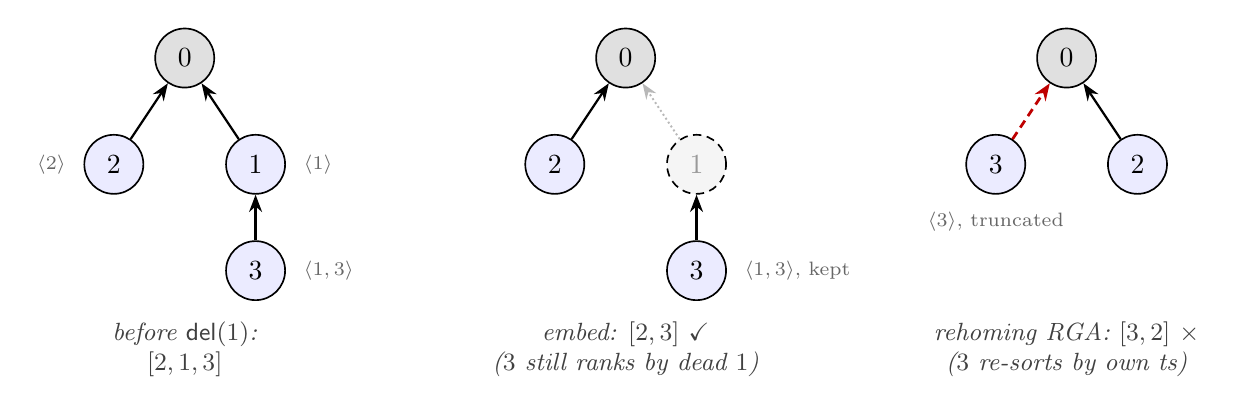
\begin{tikzpicture}
  % ---- before the delete: both designs agree
  \node[rootvtx] (br) at (0,0) {$0$};
  \node[vtx]  (b2) at (-0.9,-1.35) {$2$};
  \node[vtx]  (b1) at ( 0.9,-1.35) {$1$};
  \node[vtx]  (b3) at ( 0.9,-2.7)  {$3$};
  \draw[anc] (b2) -- (br);
  \draw[anc] (b1) -- (br);
  \draw[anc] (b3) -- (b1);
  \node[elbl, left=1mm of b2]  {$\langle 2\rangle$};
  \node[elbl, right=1mm of b1] {$\langle 1\rangle$};
  \node[elbl, right=1mm of b3] {$\langle 1,3\rangle$};
  \node[capt, align=center] at (0,-3.7)
    {before $\del(1)$:\\ $[2,1,3]$};
  % ---- embedded chain: key kept whole
  \begin{scope}[shift={(5.6,0)}]
  \node[rootvtx] (er) at (0,0) {$0$};
  \node[vtx]   (e2) at (-0.9,-1.35) {$2$};
  \node[deadv] (e1) at ( 0.9,-1.35) {$1$};
  \node[vtx]   (e3) at ( 0.9,-2.7)  {$3$};
  \draw[anc] (e2) -- (er);
  \draw[ghost] (e1) -- (er);
  \draw[anc] (e3) -- (e1);
  \node[elbl, right=1mm of e3] {$\langle 1,3\rangle$, kept};
  \node[capt, align=center] at (0,-3.7)
    {embed: $[2,3]$ \checkmark\\ ($3$ still ranks by dead $1$)};
  \end{scope}
  % ---- rehoming RGA: climb truncates the key
  \begin{scope}[shift={(11.2,0)}]
  \node[rootvtx] (fr) at (0,0) {$0$};
  \node[vtx] (f3) at (-0.9,-1.35) {$3$};
  \node[vtx] (f2) at ( 0.9,-1.35) {$2$};
  \draw[climb] (f3) -- (fr);
  \draw[anc]   (f2) -- (fr);
  \node[elbl, below=1mm of f3] {$\langle 3\rangle$, truncated};
  \node[capt, align=center] at (0,-3.7)
    {rehoming RGA: $[3,2]$ $\times$\\ ($3$ re-sorts by own ts)};
  \end{scope}
\end{tikzpicture}
\caption{The one-line separation on the L1 delete-reorder litmus:
insert $1$ and $2$ at the front, $3$ after $1$, delete $1$. The
rehoming RGA's climb (red) re-parents $3$ and re-sorts it by its \emph{own}
timestamp: the truncated key $\langle 3\rangle$ beats
$\langle 2\rangle$, and $3$ jumps over $2$. The embedded chain
$\langle 1,3\rangle$ keeps ranking $3$ by its dead parent's
timestamp: $[2,3]$, the delete-order-preserving read. Arrows point
from a node to its anchor; dashed grey = dead.}
\label{fig:l1}
\end{figure}

\paragraph{Worked example (Figure~\ref{fig:credential}).} $6$ and
$10$ concurrently insert at the
front: chains $\langle 6 \rangle$ and $\langle 10 \rangle$;
display $[10, 6]$, no arbitration, at every replica and merge order.
Type $22, 16$ under $6$: chains $\langle 6, 22 \rangle$,
$\langle 6, 16 \rangle$. Delete $6$: the records of $22$ and $16$ are
untouched and still carry $6$'s timestamp. A third party concurrently
inserts $8$ at the front: $\langle 8 \rangle$ sorts below
$\langle 10 \rangle$ and above $\langle 6, 22 \rangle$, so the display
is $[10, 8, 22, 16]$ whether $8$ arrives before or after $6$'s death
(machine-checked as the \emph{credential countermodel}, the shape that
kills every timestamp-oblivious variant, \S\ref{sec:validation}).

\begin{figure}[h]
\centering
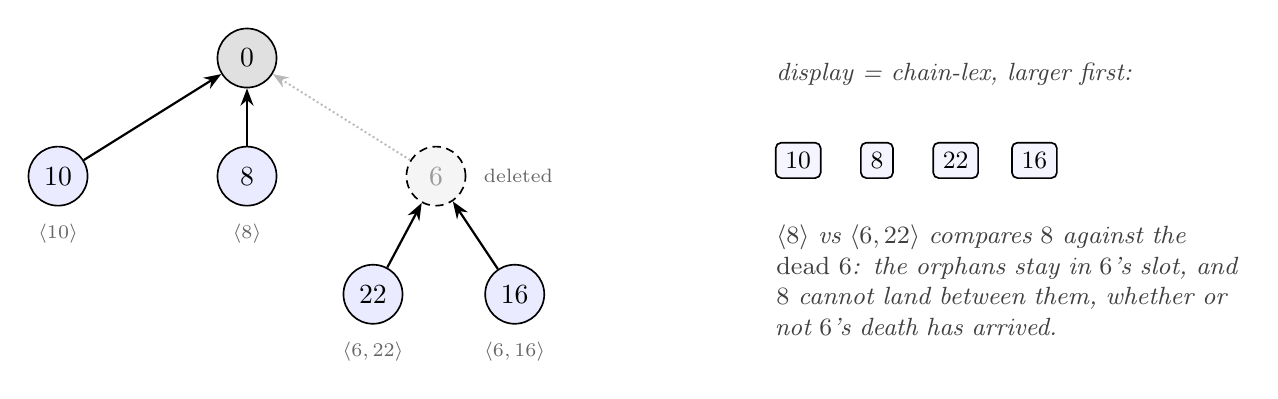
\begin{tikzpicture}
  \node[rootvtx] (r)   at (0,0)       {$0$};
  \node[vtx]     (n10) at (-2.4,-1.5) {$10$};
  \node[vtx]     (n8)  at (0,-1.5)    {$8$};
  \node[deadv]   (n6)  at (2.4,-1.5)  {$6$};
  \node[vtx]     (n22) at (1.6,-3.0)  {$22$};
  \node[vtx]     (n16) at (3.4,-3.0)  {$16$};
  \draw[anc]   (n10) -- (r);
  \draw[anc]   (n8)  -- (r);
  \draw[ghost] (n6)  -- (r);
  \draw[anc]   (n22) -- (n6);
  \draw[anc]   (n16) -- (n6);
  \node[elbl, below=1mm of n10] {$\langle 10\rangle$};
  \node[elbl, below=1mm of n8]  {$\langle 8\rangle$};
  \node[elbl, right=1mm of n6]  {deleted};
  \node[elbl, below=1mm of n22] {$\langle 6,22\rangle$};
  \node[elbl, below=1mm of n16] {$\langle 6,16\rangle$};
  \begin{scope}[shift={(7.0,-1.3)}]
    \node[capt, anchor=west] at (-0.4,1.1)
      {display = chain-lex, larger first:};
    \node[stbox] at (0,0)   {$10$};
    \node[stbox] at (1.0,0) {$8$};
    \node[stbox] at (2.0,0) {$22$};
    \node[stbox] at (3.0,0) {$16$};
    \node[capt, text width=5.9cm, align=left, anchor=north west]
      at (-0.4,-0.7)
      {$\langle 8\rangle$ vs $\langle 6,22\rangle$ compares $8$
       against the \emph{dead} $6$: the orphans stay in $6$'s slot,
       and $8$ cannot land between them, whether or not $6$'s
       death has arrived.};
  \end{scope}
\end{tikzpicture}
\caption{The credential countermodel as a birth tree. $6$ and $10$
race at the front; $22, 16$ are typed under $6$; $6$ dies; $8$
arrives at the front concurrently. Survivors sort by whole birth
chains, so the read is $[10,8,22,16]$ at every replica and merge
order. Every timestamp-oblivious variant flips this shape
(\S\ref{sec:related}).}
\label{fig:credential}
\end{figure}

\section{The representation: chains as entropy-coded coordinates}
\label{sec:encoding}

Everything above is the datatype; everything below is bits. A naive
carrier would store a full timestamp at every chain level (each
$\sim\!\log(\text{document age})$ bits, even for purely sequential
typing) and compare whole chains at every read. This section stores
the chains compactly without disturbing their order.

\paragraph{Vocabulary.} A \emph{codeword} is the bit string
$C(\delta)$ encoding one chain level: one element's timestamp,
stored as its differential $\delta$ to its birth anchor (step 1
below). A \emph{coordinate} is the bit string encoding a whole
chain: the concatenation, root to element, of one block per level
(the level's codeword plus three framing bits fixed by the mint
construction below), with nothing else marking the boundaries. We
write $|s|$ for the length in bits of a bit string $s$. Read as a
binary fraction, a coordinate names a dyadic interval in $(0,1)$;
codeword concatenation becomes interval nesting, and the interval is
the $\alpha(u)$ of Theorem~\ref{thm:faithful}. Bit string and
interval are two views of one object; we use whichever is clearer.

\paragraph{What the coding is for.} Two jobs, only one of which is
about correctness.
\emph{Job 1: cost.} The datatype layer already forced sort keys to
retain dead ancestors' timestamps (the conservation law,
\S\ref{sec:design}); the only remaining question is how many bits
that retention costs. Without entropy coding, ``tombstone-free''
would be bookkeeping: a full timestamp per level grows with document
age however calm the history. The \emph{unary control}
(\code{embed-tree}: the identical datatype with a unary code in the
mint, codeword length linear in the value, kept as the experiment's
cost-control arm; step 2 and the entropy-law table) makes the gap
measurable: 61\,KB against the coded design's 0.5\,KB on the table's
1000-element chain scenario. The coding is what makes
the headline claim true: the dead survive as the entropy of the
anchor gaps they were born across, and not more.
\emph{Job 2: faithfulness.} The chains must be stored so that plain
lexicographic bit comparison reproduces chain-lex exactly, in every
reachable state, forever. This is the single obligation the
representation owes \S\ref{sec:design}
(Theorem~\ref{thm:faithful}). Correctness lives upstairs; this layer
is an implementation that must not lie. Job 2 needs no entropy
optimality at all: it needs exactly two structural properties of the
per-level code, stated next.

\paragraph{The contract.} The stored form must support four
operations: \emph{mint} (insert: produce the new codeword from the
two timestamps alone, coordination-free, reading no siblings);
\emph{compare} (read: plain lexicographic comparison, with no tie
rule); \emph{fold} (delete: splice a dead node out by concatenating
its block into each child's stored string, exactly); and
\emph{refold} (merge: recompute survivors' coordinates by the same
concatenation). Each guarantee is bought by a specific property of
$C$:
\begin{itemize}
\item \textbf{Monotone} ($\delta < \delta' \Rightarrow C(\delta)
<_{\mathrm{lex}} C(\delta')$) buys correct \emph{compare}. A
chain-lex first difference always compares two same-anchor entries,
where timestamp order and $\delta$ order coincide (step 1); bitwise
comparison of coordinates therefore equals timestamp comparison at
the first differing level precisely when $C$ is monotone.
\item \textbf{Prefix-free} (no codeword is a prefix of another) buys
three things at once. \emph{Alignment}: in a comparison of two
coordinates, the first differing bit falls inside the first
differing level's codewords, so levels cannot be confused across
boundaries and no delimiters are needed; this is also what keeps
\emph{fold} and \emph{refold} exact splices. \emph{Geometry}: by the
Kraft correspondence, prefix-free codewords occupy pairwise-disjoint
dyadic cells, which is Theorem~\ref{thm:faithful}(i) and the reason
a concurrent front-insert can never land inside a dead sibling's
span (Figure~\ref{fig:nest}). \emph{No ties}: cell disjointness plus
Lamport uniqueness means sibling coordinates never tie, so the merge
never decides an order and the read needs no tiebreak.
\item \textbf{Universal, with a cheap floor} buys Job 1: $C$ is
defined for every $\delta \ge 1$, $|C(1)| = O(1)$ so continuation
typing costs a constant per level, and $|C(\delta)| = \Theta(\log
\delta)$ so a level pays the log of its anchor gap, whether the gap
is a race or a cursor jump (step 1), and nothing else.
\end{itemize}
Monotone plus prefix-free is all of Job 2: any such code satisfies
Theorem~\ref{thm:faithful}, which is why the Lean capstone is
parametric in the code (\S\ref{sec:mechanization}) and why the unary
control proves the same theorems at absurd cost. Entropy coding
enters only in \emph{which} monotone prefix-free code is chosen; the
choice sets the constant in the bits-per-level bill and nothing in
the correctness story. One requirement cuts across all four
operations: the arithmetic is exact, never rounded (see the binary64
refutation below).

\paragraph{Step 1: differential coding.} By causality
$\delta = x - a \ge 1$. A chain-lex first difference always compares
two entries with the \emph{same} anchor (the shared prefix), and for
a fixed anchor, ordering by $x$ and by $\delta$ coincide, so each
chain level may store the differential instead of the timestamp.
Call $\delta$ the \emph{anchor gap}: the events elapsed between the
anchor's mint and the insert's.
Continuation typing (each character anchored at its predecessor) has
$\delta = 1$ at every level regardless of how long the document has
lived. Two things widen the gap, and they pay the same bill: a
genuine race with timestamp gap $g$ costs $\log_2 g$ bits, and so
does a \emph{cursor jump}, the first character typed at an old
anchor; its successors anchor at fresh characters and are back to
$\delta = 1$. The differential is an encoding choice, not
semantics: the mathematical object remains the timestamp.

\paragraph{Step 2: entropy coding.} For $\delta \ge 1$ let $L$ be the
bit-length of $\delta$ and
\[
  C(\delta) \;=\; \underbrace{1\cdots1}_{L-1}\;0\;\bigl(\delta
  \text{ with its leading bit removed}\bigr)
  \qquad (|C(\delta)| = 2L-1),
\]
an order-preserving prefix-free code: exactly the contract. The
length accounting: prefix-freedom makes each codeword
self-delimiting, and a self-delimiting code over unbounded $\delta$
must spend bits twice, once on the value and once announcing its own
length. $C$ pays each bill at $\sim\!\log_2\delta$. The header
$1^{L-1}0$ is a unary announcement ``$L{-}1$ payload bits follow''
($L$ bits); the payload is $\delta$'s trailing $L{-}1$ bits, since
the leading bit of an $L$-bit number is always $1$: once the header
has said $L$ it carries no information and is dropped. Hence
\[
  |C(\delta)| \;=\; \underbrace{(L{-}1) + 1}_{\text{header}}
  \;+\; \underbrace{(L{-}1)}_{\text{payload}}
  \;=\; 2L - 1 \;=\; 2\lfloor \log_2 \delta \rfloor + 1,
\]
e.g.\ $C(1) = 0$, $C(2) = 100$, $C(3) = 101$, $C(5) = 11001$. This
is Elias~$\gamma$ with
its header flipped: $\gamma$ announces the length in \emph{zeros},
which is prefix-free but order-reversing across length classes:
at the first divergence the longer, hence larger, number shows a
header $0$ against the shorter's leading payload bit $1$. Writing
the header in ones makes that same position decide in favor of the
longer code, so lexicographic order on codewords is numeric order on
$\delta$. The $\gamma$-flip is the building block, not the last
word: only the \emph{value} bill is forced at $\log_2 \delta$, and
the \emph{length} bill can itself be entropy-coded. Applying $C$ to
the length field (then the payload) gives the order-preserving flip
of \textbf{Elias~$\delta$}, prefix-free and monotone by the same
across-length-class argument, at $\log_2 \delta + O(\log \log
\delta)$ per level; \emph{this is the canonical mint}.
\emph{Any} order-preserving prefix-free
code works here, and the artifact exists in three proved encodings
of one datatype (\code{embed-tree} unary, \code{embed-code} the
$\gamma$-flip, \code{eliasDeltaCode} the $\delta$-flip); the capstone
theorem is inherited at each verbatim, with zero new proof content
(\S\ref{sec:mechanization}): the code-parametricity claim,
machine-validated. Two honest footnotes: per level the $\delta$-flip
wins only from $\delta \ge 32$ and loses at $\delta \in \{2,3\} \cup
[8,15]$ (kernel-checked length comparisons), and measured editing
tails are thin, so on real traces the two flips are a wash; the
dominance shows in race-heavy shapes (the entropy-law table below)
and in the asymptotics.

\paragraph{The mint.} Writing $b = 1 \cdot C(\delta)$ (a leading 1
keeps coordinates positive) and $w = 2^{-|b|-2}$, the mint is the
second quarter of $b$'s dyadic cell:
\[
  M(\delta) \;=\; \bigl(\,0.b + w,\ \ 0.b + 2w\,\bigr)
  \;\subset\; \bigl[\,0.b,\ 0.b + 4w\,\bigr) .
\]
The quarter placement leaves a gap below and headroom above inside the
cell, and the open space $(0.b+2w,\, 0.b+4w)$ is never minted: it
exists so that the interval has room to \emph{contain} the node's own
subtree without touching the next cell. This also pins down the
per-level \emph{block} promised in the vocabulary: $0.b + w$ written
as a string is $b\,\code{01}$, so the block is
$1\,C(\delta)\,\code{01}$, the codeword in its three framing bits
(the leading $1$ for positivity, the \code{01} that selects the
second quarter). The block is what a node stores; read as a binary
fraction it is the lower endpoint of $M(\delta)$, and flipping the
trailing \code{01} to \code{10} gives the upper. Worked out for
small deltas:

\begin{center}\small
\begin{tabular}{@{}rllll@{}}
\toprule
$\delta$ & $C(\delta)$ & block $= 1\,C(\delta)\,\code{01}$ &
  $M(\delta)$ & bits/level \\
\midrule
1   & \code{0}             & \code{1001}     & $(9/16,\ 10/16)$   & 4 \\
2   & \code{100}           & \code{110001}   & $(49/64,\ 50/64)$  & 6 \\
3   & \code{101}           & \code{110101}   & $(53/64,\ 54/64)$  & 6 \\
4   & \code{11000}         & \code{11100001} & $(225/256,\ 226/256)$ & 8 \\
5   & \code{11001}         & \code{11100101} & $(229/256,\ 230/256)$ & 8 \\
10  & \code{1110010}       & \code{1111001001} & $(969/1024,\ 970/1024)$ & 10 \\
100 & \code{1111110100100} & \code{1111111010010001} &
  $(65169/65536,\ 65170/65536)$ & 16 \\
\bottomrule
\end{tabular}
\end{center}

\noindent Three things to read off. The endpoints are consecutive
dyadics at scale $2^{-(|b|+2)}$ (numerators $n$ and $n{+}1$): the
mint is one tick wide at its own scale, with the tick below it (the
gap) and the two ticks above it (the subtree headroom) never minted.
The rows are strictly increasing as fractions: monotonicity made
visible. And the bit count is $2L + 2$ for an $L$-bit $\delta$: four
bits at $\delta = 1$ (the sequential-typing constant of the entropy
law), sixteen at $\delta = 100$.

\begin{figure}[h]
\centering
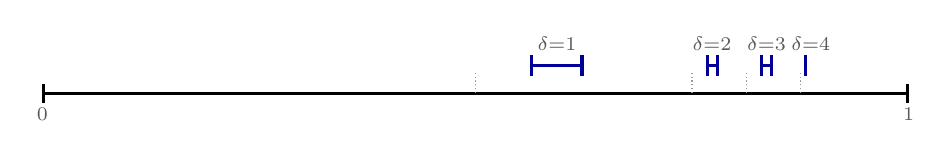
\begin{tikzpicture}[xscale=11]
  \draw[rng] (0,0) -- (1,0);
  \node[lab, below] at (0,-0.06) {$0$};
  \node[lab, below] at (1,-0.06) {$1$};
  % cells for delta = 1..4 : b = 1C(d); mint = (0.b + w, 0.b + 2w), w = 2^-(|b|+2)
  % d=1: C='0', b='10'  cell [1/2, 3/4)        mint (0.5625, 0.625)
  % d=2: C='100', b='1100' cell [3/4, 13/16)   mint (0.765625, 0.78125)
  % d=3: C='101', b='1101' cell [13/16, 7/8)   mint (0.828125, 0.84375)
  % d=4: C='11000', b='111000' cell [7/8, 57/64) mint (0.87890625, 0.8828125)
  \draw[rngB] (0.5625,0.35) -- (0.625,0.35);
  \node[lab, above] at (0.594,0.42) {$\delta{=}1$};
  \draw[rngB] (0.765625,0.35) -- (0.78125,0.35);
  \node[lab, above] at (0.773,0.42) {$\delta{=}2$};
  \draw[rngB] (0.828125,0.35) -- (0.84375,0.35);
  \node[lab, above] at (0.836,0.42) {$\delta{=}3$};
  \draw[rngB] (0.87890625,0.35) -- (0.8828125,0.35);
  \node[lab, above] at (0.887,0.42) {$\delta{=}4$};
  \draw[black!40, densely dotted] (0.5,0.0) -- (0.5,0.28);
  \draw[black!40, densely dotted] (0.75,0.0) -- (0.75,0.28);
  \draw[black!40, densely dotted] (0.8125,0.0) -- (0.8125,0.28);
  \draw[black!40, densely dotted] (0.875,0.0) -- (0.875,0.28);
\end{tikzpicture}
\caption{Mints $M(\delta)$ for $\delta = 1..4$ inside the parent's unit
interval (cell boundaries dotted). Larger deltas sit strictly higher;
distinct deltas are disjoint with gaps; each mint is a quarter of its
cell, leaving room for the node's own subtree. Drawn for the
$\gamma$-flip $C$; the construction reads verbatim over any
order-preserving prefix-free code, in particular the canonical
Elias-$\delta$ mint (step 2).}
\label{fig:mint}
\end{figure}

\paragraph{The stored state.} The carrier stores each live node
parent-relatively:
\[
  \sigma \;:\; t \;\mapsto\; (\,\mathrm{par} \in \mathbb{N},\ \
  s \in \{0,1\}^{*},\ \ \mathrm{char}\,),
\]
where $s$ is a block ($1\,C(\delta)\,\code{01}$ at birth; after
folds, below, a concatenation of blocks) \emph{relative to the
parent}, and $\mathrm{par} = 0$ denotes the root sentinel (which
owns $(0,1)$ and is never stored). The record holds no interval; the
interval is the string's decoding,
\[
  (lo, hi) \;=\; \bigl(\,0.s,\ \ 0.s + 2^{-|s|}\,\bigr)
  \;\subset\; (0,1),
\]
consecutive dyadics at $s$'s own scale, one block at a time exactly
as in the mint table. The maintenance below and
Theorem~\ref{thm:faithful} are stated on the intervals, and every
operation they perform on an interval is a string operation on $s$:
composition is concatenation, comparison is lexicographic. (The
validation model stores the decoded pair directly, as exact
fractions.) A node's \emph{absolute} interval is the affine
composition of the intervals along its parent chain. For a node $v$
with mint $M(\delta_v) = (lo_v,\ lo_v + w_v)$, let
\[
  \varphi_v : (0,1) \to M(\delta_v), \qquad
  \varphi_v(x) \;=\; lo_v + w_v \cdot x,
\]
the unique increasing affine bijection of the unit interval onto
$v$'s mint; it maps a subinterval $(a,b)$ to
$(lo_v + w_v a,\ lo_v + w_v b)$, and on strings it prefixes $v$'s
block: $\varphi_v(0.y) = 0.(s_v\, y)$. Write
\[
  \alpha(u) \;=\; \varphi_{c_1} \circ \cdots \circ
  \varphi_{c_k}\bigl(M(\delta_u)\bigr)
\]
for the composition along $u$'s birth chain $c_1 \cdots c_k\,u$
($\delta_v$ is $v$'s delta to its birth parent): $\alpha(u)$ is the
\emph{encoding of $\chain(u)$}, and at the string level it decodes
the concatenation of the blocks along the chain. Worked on the tree
of Figure~\ref{fig:credential}, redrawn before $\del(6)$ with the
delta (child minus anchor) on each edge and the stored block under
each node:

\begin{center}
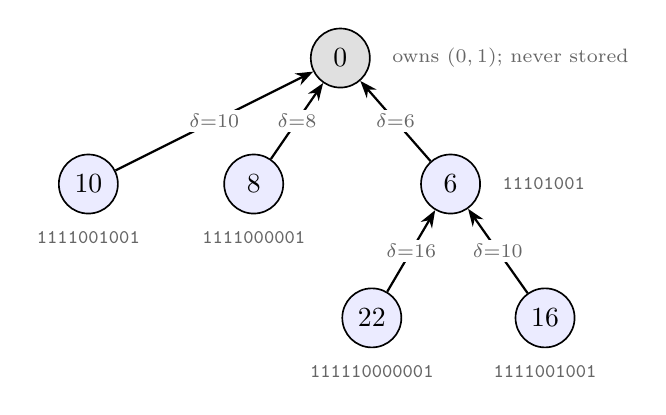
\begin{tikzpicture}
  \node[rootvtx] (r)   at (0,0)        {$0$};
  \node[elbl, right=1.5mm of r] {owns $(0,1)$; never stored};
  \node[vtx] (n10) at (-3.2,-1.6) {$10$};
  \node[vtx] (n8)  at (-1.1,-1.6) {$8$};
  \node[vtx] (n6)  at (1.4,-1.6)  {$6$};
  \node[vtx] (n22) at (0.4,-3.3)  {$22$};
  \node[vtx] (n16) at (2.6,-3.3)  {$16$};
  \draw[anc] (n10) -- (r)
    node[elbl, midway, fill=white, inner sep=1.5pt] {$\delta{=}10$};
  \draw[anc] (n8) -- (r)
    node[elbl, midway, fill=white, inner sep=1.5pt] {$\delta{=}8$};
  \draw[anc] (n6) -- (r)
    node[elbl, midway, fill=white, inner sep=1.5pt] {$\delta{=}6$};
  \draw[anc] (n22) -- (n6)
    node[elbl, midway, fill=white, inner sep=1.5pt] {$\delta{=}16$};
  \draw[anc] (n16) -- (n6)
    node[elbl, midway, fill=white, inner sep=1.5pt] {$\delta{=}10$};
  \node[elbl, below=1mm of n10] {\code{1111001001}};
  \node[elbl, below=1mm of n8]  {\code{1111000001}};
  \node[elbl, right=1.5mm of n6] {\code{11101001}};
  \node[elbl, below=1mm of n22] {\code{111110000001}};
  \node[elbl, below=1mm of n16] {\code{1111001001}};
\end{tikzpicture}
\end{center}

\noindent Writing $(n, n{+}1)/2^{k}$ for the interval
$(n/2^k,\ (n{+}1)/2^k)$ and $\approx$ for its lower endpoint:

\begin{center}\small
\setlength{\tabcolsep}{4.5pt}
\begin{tabular}{@{}rrllll@{}}
\toprule
node & $\delta$ & stores $(\mathrm{par}, s)$ & decode of $s$ &
  $\alpha$ (absolute) & $\approx$ \\
\midrule
$10$ & $10$ & $(0,\ \code{1111001001})$   & $(969, 970)/2^{10}$ &
  $(969, 970)/2^{10}$ & $0.94629$ \\
$8$  & $8$  & $(0,\ \code{1111000001})$   & $(961, 962)/2^{10}$ &
  $(961, 962)/2^{10}$ & $0.93848$ \\
$6$  & $6$  & $(0,\ \code{11101001})$     & $(233, 234)/2^{8}$  &
  $(233, 234)/2^{8}$  & $0.91016$ \\
$22$ & $16$ & $(6,\ \code{111110000001})$ & $(3969, 3970)/2^{12}$ &
  $(958337, 958338)/2^{20}$ & $0.91394$ \\
$16$ & $10$ & $(6,\ \code{1111001001})$   & $(969, 970)/2^{10}$ &
  $(239561, 239562)/2^{18}$ & $0.91385$ \\
\bottomrule
\end{tabular}
\end{center}

\noindent The root's children store their absolute intervals already
($\mathrm{par} = 0$). The grandchildren compose: $22$'s absolute
string is its parent's block followed by its own,
\code{11101001}\,\code{111110000001} ($20$ bits, hence the
$2^{20}$), and likewise $16$'s ($18$ bits). Both absolute intervals
sit inside $M(6) = (0.91016, 0.91406)$ while $8$'s sits above it, so
the descending-$\alpha$ read is $[10, 8, 22, 16]$ and $8$ cannot
land between the orphans. Nodes $16$ and $10$ store the same
string, both being $\delta = 10$ births; records are
parent-relative, so this is no collision. After $\del(6)$ the fold
rewrites the two records to $(\mathrm{par}\ 0,\ \text{the
concatenated } s)$ and the $\alpha$ column is unchanged bit for bit.
Figure~\ref{fig:nest} draws these intervals (widths schematic).

\begin{figure}[h]
\centering
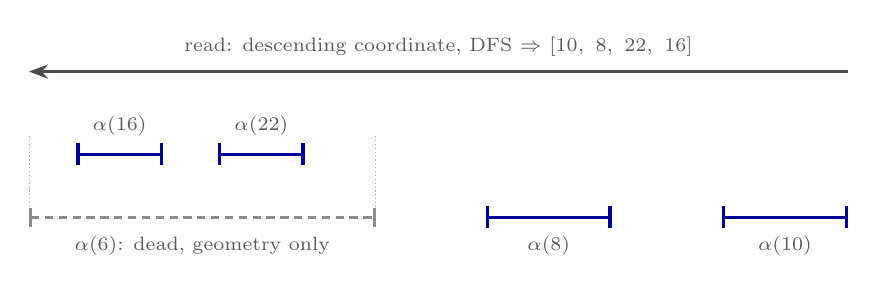
\begin{tikzpicture}
  % depth-1 intervals (schematic widths; true mints are dyadic, Fig mint)
  \draw[rngD] (0.6,0) -- (5.0,0);
  \node[lab, below] at (2.8,-0.12) {$\alpha(6)$: dead, geometry only};
  \draw[rngB] (6.4,0) -- (8.0,0);
  \node[lab, below] at (7.2,-0.12) {$\alpha(8)$};
  \draw[rngB] (9.4,0) -- (11.0,0);
  \node[lab, below] at (10.2,-0.12) {$\alpha(10)$};
  % depth-2 mints, nested inside alpha(6)
  \draw[rngB] (1.2,0.8) -- (2.3,0.8);
  \node[lab, above] at (1.75,0.92) {$\alpha(16)$};
  \draw[rngB] (3.0,0.8) -- (4.1,0.8);
  \node[lab, above] at (3.55,0.92) {$\alpha(22)$};
  \draw[black!35, densely dotted] (0.6,0.08) -- (0.6,1.05);
  \draw[black!35, densely dotted] (5.0,0.08) -- (5.0,1.05);
  % read direction
  \draw[-{Stealth[length=2.4mm]}, line width=0.9pt, black!70]
    (11.0,1.85) -- (0.6,1.85);
  \node[lab, above] at (5.8,1.92)
    {read: descending coordinate, DFS $\Rightarrow$ $[10,\ 8,\ 22,\ 16]$};
\end{tikzpicture}
\caption{Figure~\ref{fig:credential} downstairs (widths schematic;
true mints are the dyadic cells of Figure~\ref{fig:mint}). Deleting
$6$ removes its record, but $\alpha(16)$ and $\alpha(22)$ are
compositions \emph{through} $M(6)$: the dead node survives as the
dashed container, the tombstone compressed into geometry. $8$'s
interval can never land inside $\alpha(6)$'s span: distinct deltas
occupy disjoint cells (Theorem~\ref{thm:faithful}(i)), which is the
credential verdict, now a fact about intervals.}
\label{fig:nest}
\end{figure}

\paragraph{Maintenance.} How the stored form tracks the datatype:
\begin{itemize}
\item $\ins(x \leftarrow a)$ mints $M(x - a)$ relative to $a$: the
new record depends only on the two timestamps.
\item $\del(d)$ \emph{isometrically folds} $d$ into its children:
each child $c$ is re-parented to $d$'s parent and $d$'s record is
substituted into $c$'s. On the stored strings this is concatenation,
$c.s := d.s\, c.s$; read as intervals, $c.\mathrm{frac} :=
d.\mathrm{frac} \circ c.\mathrm{frac}$, where $I \circ J$ is the
image of $J$ under the increasing affine bijection of $(0,1)$ onto
$I$ (the $\varphi$ of the stored state, with $I$ in place of a
mint): for $I = (lo,\ lo + w)$,
\[
  I \circ J \;=\; (\,lo + w \cdot lo_J,\ \ lo + w \cdot hi_J\,).
\]
The substitution is exact. Upstairs, deletion
changes nobody's sort key (\S\ref{sec:design}); the fold is the
parent-relative storage scheme \emph{re-normalizing} while every
absolute interval stays fixed (Figure~\ref{fig:fold}):
representation maintenance, not datatype semantics. On the running
example, $\del(6)$ removes $6$'s record and substitutes it into both
children: $22$'s record $(6,\ \code{111110000001})$ becomes
$(0,\ \code{11101001}\,\code{111110000001})$, whose decode is
\begin{align*}
  (233, 234)/2^{8} \circ (3969, 3970)/2^{12}
  &= (233 \cdot 2^{12} + 3969,\ 233 \cdot 2^{12} + 3970)/2^{20}\\
  &= (958337, 958338)/2^{20},
\end{align*}
and likewise $16$'s becomes $(0,\
\code{11101001}\,\code{1111001001})$, decoding $(239561,
239562)/2^{18}$. Both are exactly the $\alpha$ column of the worked
table: the absolute intervals did not move, only the
parent-relative bookkeeping did.
\item The merge \emph{refolds}: for each survivor, compute its
absolute interval by folding its record to the root inside the input
that holds it (a record's stored parent is always live in its own
input, so the chain stays in one input; by
Theorem~\ref{thm:faithful}(iii) the choice of input cannot matter,
asserted at runtime and never fired); re-parent to the nearest
\emph{surviving} ancestor; re-relativize.
\item The read is depth-first from the root, children in descending
order of $lo$. No tie rule is needed (Corollary~\ref{cor:lex}).
\end{itemize}

\begin{figure}[h]
\centering
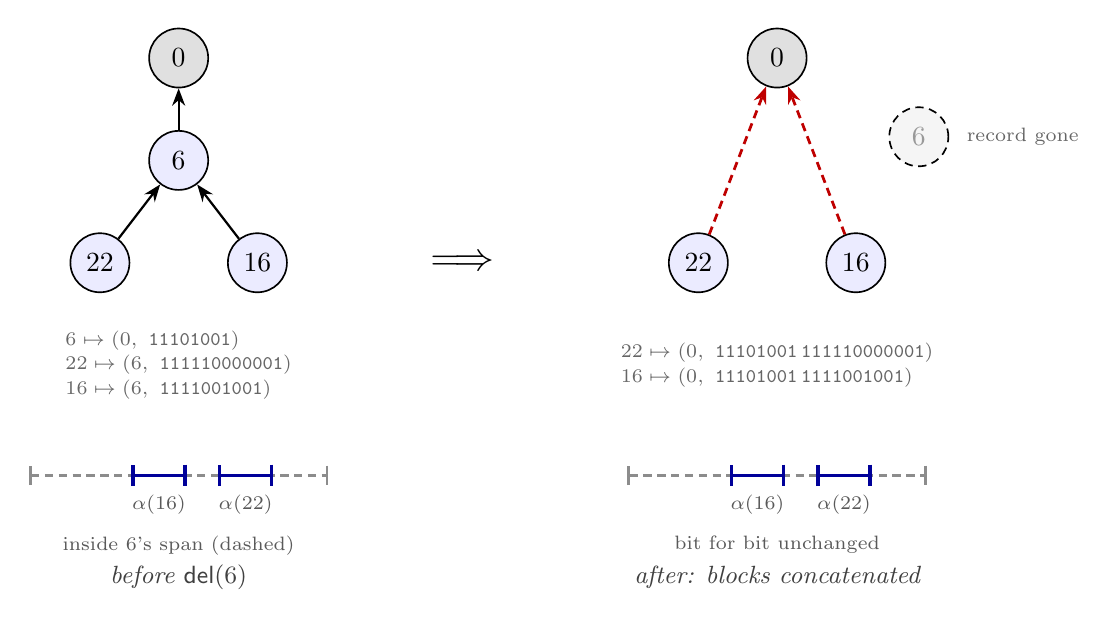
\begin{tikzpicture}
  % ---- before del(6): parent-relative records
  \node[rootvtx] (ar)  at (0,0)     {$0$};
  \node[vtx]     (a6)  at (0,-1.3)  {$6$};
  \node[vtx]     (a22) at (-1.0,-2.6) {$22$};
  \node[vtx]     (a16) at ( 1.0,-2.6) {$16$};
  \draw[anc] (a6)  -- (ar);
  \draw[anc] (a22) -- (a6);
  \draw[anc] (a16) -- (a6);
  \node[elbl, align=left] at (0,-3.9)
    {$6  \mapsto (0,\ \code{11101001})$\\[1pt]
     $22 \mapsto (6,\ \code{111110000001})$\\[1pt]
     $16 \mapsto (6,\ \code{1111001001})$};
  \draw[rngD] (-1.9,-5.3) -- (1.9,-5.3);
  \draw[rngB] (-0.6,-5.3) -- (0.1,-5.3);
  \draw[rngB] ( 0.5,-5.3) -- (1.2,-5.3);
  \node[lab, below] at (-0.25,-5.42) {$\alpha(16)$};
  \node[lab, below] at ( 0.85,-5.42) {$\alpha(22)$};
  \node[lab, below] at (0,-5.95) {inside $6$'s span (dashed)};
  \node[capt] at (0,-6.6) {before $\del(6)$};
  % ---- arrow
  \node at (3.6,-2.6) {\Large $\Longrightarrow$};
  % ---- after: blocks concatenated, absolute intervals fixed
  \begin{scope}[shift={(7.6,0)}]
  \node[rootvtx] (br)  at (0,0)     {$0$};
  \node[deadv]   (b6)  at (1.8,-1.0) {$6$};
  \node[elbl, right=1mm of b6] {record gone};
  \node[vtx]     (b22) at (-1.0,-2.6) {$22$};
  \node[vtx]     (b16) at ( 1.0,-2.6) {$16$};
  \draw[climb] (b22) -- (br);
  \draw[climb] (b16) -- (br);
  \node[elbl, align=left] at (0,-3.9)
    {$22 \mapsto (0,\ \code{11101001}\,\code{111110000001})$\\[1pt]
     $16 \mapsto (0,\ \code{11101001}\,\code{1111001001})$};
  \draw[rngD] (-1.9,-5.3) -- (1.9,-5.3);
  \draw[rngB] (-0.6,-5.3) -- (0.1,-5.3);
  \draw[rngB] ( 0.5,-5.3) -- (1.2,-5.3);
  \node[lab, below] at (-0.25,-5.42) {$\alpha(16)$};
  \node[lab, below] at ( 0.85,-5.42) {$\alpha(22)$};
  \node[lab, below] at (0,-5.95) {bit for bit unchanged};
  \node[capt] at (0,-6.6) {after: blocks concatenated};
  \end{scope}
\end{tikzpicture}
\caption{The isometric fold on the running example. $\del(6)$
deletes $6$'s record and concatenates its block \code{11101001}
onto the front of each child's, re-parenting both to the root (red:
the re-parenting, a storage move only). The stored states change:
$22$ and $16$ now carry two-block strings and $\mathrm{par}\ 0$.
The absolute intervals $\alpha(22) = (958337, 958338)/2^{20}$ and
$\alpha(16) = (239561, 239562)/2^{18}$, and with them the display,
are bit-for-bit unchanged: upstairs, the sort keys still read
$\langle 6, 22\rangle$ and $\langle 6, 16\rangle$. The dashed span
is $6$'s old interval, surviving as pure geometry.}
\label{fig:fold}
\end{figure}

\paragraph{Why the codeword must announce its own end.} Before the
theorem, the countermodel that motivates it. A single codeword in a
field of known extent needs no header, and the length looks
recoverable from the string itself; plain binary shows what breaks,
once per purchase in the contract. \emph{Geometry:} $B(2) = \code{10}$
prefixes $B(5) = \code{101}$, so $B(5)$'s cell sits inside $B(2)$'s;
containment means ancestry, so the $\delta{=}5$ sibling lands amid
the $\delta{=}2$ sibling's descendants and non-interleaving dies
with everything alive. \emph{Parsing:} once a fold erases the
structural boundary between blocks, \code{101100\ldots} reads as
$B(2)$ then \code{11\ldots} or as $B(5)$ then \code{00\ldots}, and
nothing outside the string can say. \emph{Ties:} a binary fraction
cannot see trailing zeros, so \code{10} and \code{100} both denote
$\tfrac12$; distinct siblings mint touching intervals, and the id
tiebreak wakes into an arbiter that orders by id, not chain-lex.
Nor can the header bits be dodged: prefix-freedom demands
$\sum_\delta 2^{-\ell(\delta)} \le 1$, and plain binary puts
$2^{L-1}$ values at every length $L$, so every prefix-free code
pays a length announcement of order $\log L$ somewhere (out-of-band
boundary tables cost the same bits and forfeit the string as a
self-contained key; database key encodings inline it for the same
reason). And the fold names where the boundary went: the tree node
that carried it structurally is the deleted tombstone, whose
ordering verdict becomes the payload and whose boundary becomes the
header. ``Tombstone compressed into coordinate entropy'' is literal
at the bit level.

\paragraph{The one obligation.} The four theorems of the earlier
drafts collapse into a single statement about the encoding.

\begin{theorem}[encoding faithfulness]\label{thm:faithful}
\begin{itemize}
\item[(i)] \emph{Order-embedding at one level:} for $\delta \ne
\delta'$, $M(\delta)$ and $M(\delta')$ are disjoint with a gap;
$\delta < \delta' \Rightarrow M(\delta)$ lies entirely below
$M(\delta')$.
\item[(ii)] \emph{Homomorphism:} $\alpha$ realizes chain
concatenation as affine composition and embeds chain-lex in the
interval order: for distinct $u, v$, if $\chain(u)$ is a proper
prefix of $\chain(v)$ then $\alpha(v) \subset \alpha(u)$ (and, if
both are live, the two are never read-time siblings); otherwise
$\alpha(u) \cap \alpha(v) = \varnothing$, with the chain-lex-greater
element's interval strictly higher.
\item[(iii)] \emph{Exact maintenance:} in every reachable state,
every live node's stored records compose to exactly $\alpha(u)$.
\end{itemize}
\end{theorem}
\begin{proof}
(i) $C$ is prefix-free: codes of lengths $2L{-}1 < 2M{-}1$ differ at
position $L$ (the shorter's header terminator $0$ against the longer's
header $1$); equal-length codes differ in the payload. Prefix-free
codes have pairwise-disjoint dyadic cells. $C$ is monotone as a binary
fraction: within a length class the payload is $\delta$'s low bits in
order; across classes the position-$L$ bit decides in favor of the
longer code. Disjoint cells ordered by their codes, and mints interior
quarters of their cells, give both claims.
(ii) If neither chain is a prefix of the other, they first differ on
distinct deltas relative to the \emph{same} birth ancestor
(\S\ref{sec:encoding}, step 1); (i) separates them there, and affine
images of disjoint intervals are disjoint and order-preserved (each
$\varphi$ is increasing). If $\chain(u)$ prefixes $\chain(v)$, then
$\alpha(v) \subseteq \varphi_{c_1} \circ \cdots \circ
\varphi_{c_k}(\varphi_u((0,1))) = \alpha(u)$ by construction; and if
both are live, $v$'s nearest live ancestor is $u$ or deeper, so
they never share a current parent, and sibling groups are pairwise
disjoint.
(iii) By induction over transitions. $\ins$ establishes it by
definition. $\del$'s fold replaces $(\mathrm{par}, \mathrm{frac})$
pairs by their exact composition, leaving $\alpha$ unchanged. The merge
recomputes precisely $\alpha(u)$ (folding a record chain to the root)
and re-relativizes against another $\alpha$; ties cannot exist by
(i) and (ii), so no step of any transition ever rewrites an interval
by anything but exact composition.
\end{proof}

\begin{corollary}[display $\equiv$ chain-lex; no tie rule]
\label{cor:lex}
The read (DFS by descending $lo$) enumerates survivors in exactly
chain-lex order: per level, larger delta first, so among same-parent
siblings, exactly newest first; survivors rank by their own
timestamps, folded heirs by their dead founder's. Sibling $lo$-values
never tie; the read's id tiebreak is dead code. Machine checks:
pairwise sibling disjointness asserted at every read of $320$
randomized executions, all clean; over $19{,}531$ multi-member sibling
groups, own-timestamp order violated $3{,}481$ times (exactly the
post-fold heir groups; forcing own-ts there is the refuted
dissolution behavior), \textbf{chain-lex violated $0$ times}.
\end{corollary}

\paragraph{The entropy law.} A coordinate is the concatenation of the
codes along the birth chain: $\Theta(\sum_i \log \delta_i)$ bits,
the entropy of the chain. Continuation typing ($\delta = 1$ at every
level) costs $\sim$4 bits per level under every code here; a level
minted across an event gap $g$, by a race or by the first character
after a cursor jump, costs $\log_2 g + O(\log \log g)$ bits under
the canonical Elias-$\delta$ mint ($2\log_2 g + 1$ under the
$\gamma$-flip). \emph{The state pays for the magnitude of edit
non-locality, concurrent or not, and for nothing else.} Measured (1000
elements; the numbers are \emph{order metadata alone}, survivors'
coordinate bits read off the dyadic denominators; characters are
excluded, since data costs are identical across all designs):

\begin{center}\small
\setlength{\tabcolsep}{4.5pt}
\begin{tabular}{@{}lcccc@{}}
\toprule
scenario & \shortstack[c]{quarter carve\\ (refuted)} &
  unary mint & $\gamma$-flip mint & \textbf{Elias-$\delta$ mint} \\
\midrule
chain then delete-all ($\delta{=}1$) & $2^{2001}$ &
  $2^{502501}$ ($\sim$61 KB) & $2^{4001}$ ($\sim$0.5 KB) &
  $\boldsymbol{2^{4001}}$ ($\sim$0.5 KB) \\
1000 root siblings ($\delta{=}t$) & --- (ties) &
  max $2^{1003}$, 125 KB & max $2^{23}$, 5 KB &
  \textbf{max $\boldsymbol{2^{20}}$, 4 KB} \\
\bottomrule
\end{tabular}
\end{center}

\paragraph{The carrier.} The natural representation is a
\textbf{parent-relative bit string per node}: the fold is
concatenation, comparison is lexicographic ($O(1)$-ish with
structure sharing); the rationals are the semantics of the strings,
kept for the proofs. Nothing here computes $M(\delta)$: the
endpoints $0.b + w$ and $0.b + 2w$ are the strings $b\,\code{01}$
and $b\,\code{10}$, so the mint emits a block and the fold
concatenates, and $hi$ need not be stored at all. The Lean
mechanization drops even the framing bits: its coordinate is the
bare codeword concatenation on \code{List Bool} (\code{mint} appends
$\Gamma.\mathrm{enc}(t - a)$ to the anchor's coordinate), with the
prefix rule stated directly on strings; the quarter framing serves
the interval realization alone, buying positivity and subtree
interiority. The rational $M(\delta)$ is computed in exactly one
place, the validation model \code{embed\_tree.py}, as exact
fractions; the entropy tables read their bit counts off those
denominators. IEEE 754 binary64 is machine-refuted as the
carrier, a faithfulness failure rather than a design failure: mints
degenerate at $t = 52$, depths underflow at 44, and rounding voids
Theorem~\ref{thm:faithful}(iii) (6/120 PBT executions die). The
obstruction is a pigeonhole (chains carry $\Theta(\sum \log
\delta)$ bits; a fixed-width word holds 64), but binary64 is sound
as a \emph{comparison cache} with exact fallback on float equality.

\paragraph{Timestamps in practice.} The unique stamps in
$\mathbb{N}^{+}$ are Lamport's 1978 construction, flattened: each
replica ticks a counter per local operation, advances it to the max
on merge, and breaks ties by replica id, packed as
$t \cdot 2^{k} + r$ with $k$ id bits. Uniqueness and causality
($t_a < t_x$ gives $\mathrm{packed}_a < \mathrm{packed}_x$ regardless
of ids, so $\delta \ge 1$) both survive the packing; the proof layer
only \emph{assumes} uniqueness (the Lamport-structural part of
honesty), and this construction is the witness that the assumption is
realizable. Two entropy caveats. \emph{(i)} Packing inflates every
delta by $2^{k}$, costing $\sim$$2k$ extra bits per chain level, which
turns the 0.5 KB sequential run above into $\sim$3 KB at $k = 10$.
Cheaper: extend the mint's code to the pair, $C(\Delta t)$ followed
by a $k$-bit id. The pair code is still order-preserving prefix-free
(lex on $(\Delta t, r)$), and costs $k$ bits only where the level is
minted. A further option, unvalidated against the battery and
recorded as a design note, is to order sibling ids \emph{relative to
the anchor's} (any deterministic per-anchor id order is a legitimate
tiebreak; convergence needs agreement, not a uniform order), making
``same author as my anchor'', i.e.\ sequential typing, cost $\sim$1
bit, so only genuine cross-author races pay $\log R$. \emph{(ii)} The
clock must be \emph{dense logical time, never physical}: wall-clock
or HLC stamps make $\delta$ measure elapsed time rather than elapsed
events: a keystroke every 100\,ms over $\mu$s-resolution stamps
mints $\delta \approx 10^{5}$, $\sim$34 bits per level for a purely
sequential edit. The entropy law holds precisely because the counter
ticks once per event, making $\delta$ an event-count gap; if
wall-clock order is ever wanted, it belongs in a display-layer
tiebreak, never in the minted coordinate.

\paragraph{What remains open.} Dead chain entries concatenated into
survivors' strings are the conservation law's irreducible content
(\S\ref{sec:design}); reclaiming them under \emph{causal stability}
(renumber once every replica has seen the delete, the only
condition under which rewriting geometry is safe, since no verdict
involving the dead can be contested again) is the deepest of the
open cost items, and it is orthogonal to correctness. The wider
compression headroom is catalogued with its research questions in
the companion assessment
\code{whiteboard/order-coding-compression-notes.md}:
context-conditioned per-anchor codes (licensed by comparison
locality: a chain-lex first difference never crosses anchors),
coalescing $\delta{=}1$ runs, Steiner-sharing dead prefixes across
co-heirs, stability-gated rank re-coding, and the Elias-$\delta$
constant (step 2 above).

\section{The insert prefix: for the proof, and the proof alone}
\label{sec:prefix}

The insert payload $\pi$ exists for verification, not execution.
This section says why it must exist, and why an implementation may
drop it from the wire.

\paragraph{Why $\rcrel$ must be \Either.} The verification framework
(Part~I) resolves a concurrent pair of
non-commuting operations by consulting a declared
conflict-resolution order $\rcrel$; any \emph{oriented} entry for an
insert/delete pair, however, incurs a base commutation obligation
that is machine-refuted for this design space: ordering
$\ins(x \leftarrow a)$ against $\del(a)$ (in either direction) is
undischargeable as a conflict entry, because rehoming is
non-transitive across chains of deletions. So $\rcrel = \Either$: the
proof must show the two \emph{commute}, in both orders, on all
applicable states.

\paragraph{The commutation, and where the prefix earns its keep.}
Order 1, $\ins(x \leftarrow a)$ then $\del(a)$: $x$ is born with
chain $\pi \cdot x$, and the delete touches no chain (downstairs: the
fold re-homes $x$'s record with composed coordinates; by exactness
$\alpha(x) = \alpha(a) \circ M(x - a)$). Order 2, $\del(a)$ then
$\ins(x \leftarrow a)$: $a$ is gone; application must still be
\emph{total} and land $x$ on the same sort key. This is what the
carried prefix $\pi = \chain(a)$ (equivalently, the anchor's
coordinate) provides: apply sets
$\chain(x) = \pi \cdot x$ (downstairs:
$\alpha(x) = \pi \circ M(x - a)$, attached to the nearest live
ancestor). The two orders produce \emph{equal} states: commutation
to equality, not merely up to $\approx$, courtesy of canonicity
(Theorem~\ref{thm:chain}). Figure~\ref{fig:commute} draws the square
on the smallest instance.

\begin{figure}[h]
\centering
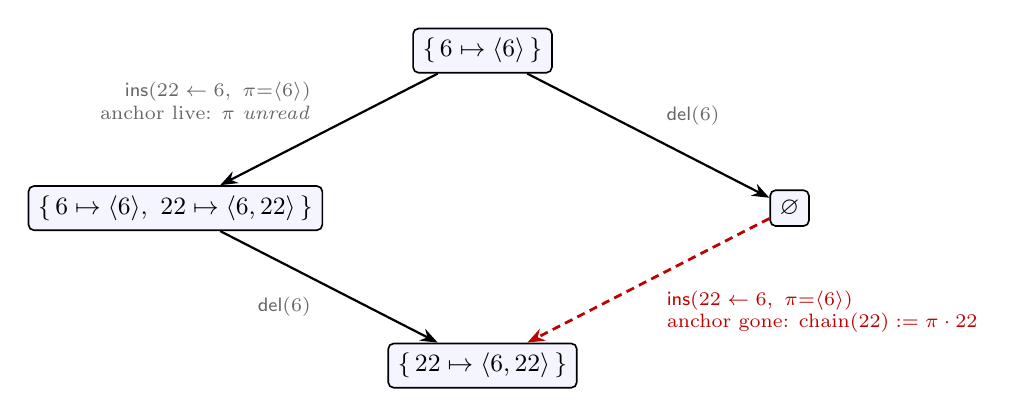
\begin{tikzpicture}
  \node[stbox] (s0) at (0,0)      {$\{\,6 \mapsto \langle 6\rangle\,\}$};
  \node[stbox] (sl) at (-3.9,-2.0)
    {$\{\,6 \mapsto \langle 6\rangle,\ 22 \mapsto \langle 6,22\rangle\,\}$};
  \node[stbox] (sr) at (3.9,-2.0) {$\varnothing$};
  \node[stbox] (sb) at (0,-4.0)   {$\{\,22 \mapsto \langle 6,22\rangle\,\}$};
  \draw[anc] (s0) -- (sl)
    node[elbl, midway, above left=0mm and 1mm, align=right]
    {$\ins(22 \leftarrow 6,\ \pi{=}\langle 6\rangle)$\\ anchor live: $\pi$ \emph{unread}};
  \draw[anc] (sl) -- (sb)
    node[elbl, midway, below left=0mm and 1mm] {$\del(6)$};
  \draw[anc] (s0) -- (sr)
    node[elbl, midway, above right=0mm and 1mm] {$\del(6)$};
  \draw[climb] (sr) -- (sb)
    node[elbl, midway, below right=0mm and 1mm, align=left,
         text=red!75!black]
    {$\ins(22 \leftarrow 6,\ \pi{=}\langle 6\rangle)$\\
     anchor gone: $\chain(22) := \pi \cdot 22$};
\end{tikzpicture}
\caption{$\rcrel = \Either$ discharged: $\ins(22 \leftarrow 6)$ and
$\del(6)$ commute \emph{to equality}. Down the left, the anchor is
live and application never consults $\pi$ (the reachable, honest
order). Down the right, $6$ is already gone: the state cannot
supply the anchor's chain, so the carried $\pi = \chain(6)$ does,
landing $22$ on the same sort key. The right-hand state is
unreachable under honesty; the verification condition quantifies
over it anyway, and $\pi$ exists exactly to make that corner total.}
\label{fig:commute}
\end{figure}

\paragraph{Ghost, in the strict sense.} On every reachable state the
anchor is live at application (honesty), and the application reads
only the state and the two timestamps: $\pi$ is never consulted. The
Lean artifact carries this as \code{ins\_prefix\_ghost}
(\code{Sal/MRDTs/RGA\_Embed/RGA\_Embed\_MRDT.lean}): on accurate
ops the always-$\pi$ transition and the state-reading transition are
literally the same function: the two conventions of this section
coincide on every honest state. An implementation may therefore drop
$\pi$ from the wire
entirely; the \emph{proof} may not, because the verification
conditions quantify over reorderings that visit unreachable states,
and there application without $\pi$ is partial. The prefix costs
$O(\sum \log \delta)$ bits, the same entropy as the coordinate
itself, and exists at the proof layer alone.

\section{Validation}
\label{sec:validation}

All numbers reproduce from \code{whiteboard/litmus/} in the
accompanying Sal repository
(\code{embed\_tree.py}; harnesses \code{litmus.py}, \code{pbt.py}).
Notation: RGA$_\dagger$ is the published tombstoned RGA (Roh et
al.; \S\ref{sec:related}); the \emph{rehoming} RGA is the
convergence-verified flat tombstone-free design of \S\ref{sec:design}
(since demoted repo-wide: the L1 row below was generalized into the
kernel-checked sequential refutation of Part~III,
\S\ref{sec:refuted}, and this design took the canonical
seat). The L1--L25
battery is the litmus suite accumulated over this project's
design sweep; each entry is the named countermodel that killed at
least one of 16 prior candidate designs. The one exception below,
L19, is discharged by the sided generalization of \S\ref{sec:sided}.

\begin{center}\small
\begin{tabular}{@{}ll@{}}
\toprule
check & verdict \\
\midrule
litmus battery L1--L25 (incl.\ every countermodel that killed & clean,
  except one-sided L19 \\
\quad 16 prior designs: ceiling escapes, tie inheritance, three- &
  (backward-run interleaving, \\
\quad branch topology, frame mixing, fold-verdict inheritance) &
  the published RGA's own anomaly) \\
credential countermodel (tie heirs vs mid-ts third party, & converges,
  no flips; \\
\quad death-before vs death-after topologies) & $=$ RGA$_\dagger$'s
  reads \\
subordination-escape and retroactive-subordination CEs & survive \\
randomized version-DAG PBT (FLIP / CONV / LIVE / DUP) & 120/120 and
  300/300 clean \\
per-read sibling-disjointness assertion sweep & 320/320 clean \\
chain-lex instrumentation (19{,}531 sibling groups) & 0 violations \\
\textbf{lockstep vs the published tombstoned RGA} &
  \textbf{read-equal at every} \\
 & \textbf{apply/merge/read, 120/120} \\
L1 delete-reorder vs the verified rehoming RGA & embed $[2,3]$
  \checkmark\ vs \\
 & rehoming $[3,2]$ $\times$ \\
\bottomrule
\end{tabular}
\end{center}

\noindent The lockstep row is the identification: \emph{the
embedded-chain RGA is observationally the published tombstoned RGA
with the tombstone set compressed into coordinate entropy},
machine-checked on 120 executions and now a kernel-checked theorem
(the compaction theorem, \S\ref{sec:mechanization}): on every honest
event set, any enumeration of the tombstoned RGA's visible ids in its
own visible order \emph{equals} the embed read, element for element. The L1 row is the separation
from the verified rehoming RGA, and it is
exactly the one-line difference of \S\ref{sec:design}: that design's
climb re-sorts a rehomed node by its own timestamp (the
$[b,a,c] \to [c,b]$ anomaly), i.e.\ its sort key is the birth chain
\emph{truncated at each rehoming}; this design keeps the chain whole.

\section{The sided generalization: two-sidedness as a parameter}
\label{sec:sided}

The one blemish in the battery is L19: two replicas that each type a
\emph{backward} run at the same place (repeatedly ``insert before the
current head'') interleave, because every insert-before anchors at the
same left neighbor and both runs land in one sibling group. The fan is
not a traversal artifact: no read order of the same birth tree un-fans
a fan, so any fix must change where insert-before \emph{anchors}. The
Fugue family's answer is a second side: insert-before anchors at the
\emph{right} neighbor as an L-entry, so a backward run is a chain,
exactly as a forward run already is.

\paragraph{The L19 example, concretely.} It is the battery's own trace
(Figure~\ref{fig:sided-l19}). The LCA document is $\langle 1 \rangle$
(one insert, stamp $1$, anchored at the start marker $\diamond$). Then,
concurrently, replica A types a backward run at the head, three
inserts each anchored ``before the current first element'':
\[
  \ins(10 \text{ at head}),\quad \ins(30 \text{ at head}),\quad
  \ins(50 \text{ at head}),
\]
so A locally reads $\langle 50, 30, 10, 1 \rangle$; replica B does the
same with stamps $21, 41, 61$ and locally reads
$\langle 61, 41, 21, 1 \rangle$. (The stamps interleave numerically,
$10 < 21 < 30 < 41 < 50 < 61$, because the two replicas' Lamport
clocks advance together.) In the one-sided datatype, ``insert at the
head'' can only anchor at the left neighbor, which is $\diamond$ for
every one of the six inserts: all six become R-children of $\diamond$,
one sibling group, and the sibling tiebreak (newest first) merges the
two runs by stamp:
\[
  \langle\, 61, 50, 41, 30, 21, 10, 1 \,\rangle
\]
after the merge, the two sentences shuffled together. No traversal of
that tree can do better; the information ``these three form one run''
is simply not in a sibling fan whose stamps interleave.

\paragraph{The sided datatype, and why it prevents the interleaving.}
The generalization does not build a second datatype. An insert names an
anchor \emph{and a side}; chains become sequences of
$(\mathrm{side}, \mathrm{timestamp\ delta})$ entries; and the display
rule generalizes from the prefix rule (``a prefix precedes its
extensions'') to the in-order rule (``L-extensions, then the node, then
R-extensions''). One marker trick makes this ordinary lexicographic
comparison again: a node's sort key is its coordinate followed by a
virtual terminator, and the sided symbol alphabet is ordered
\[
  (R,1) < (R,2) < \cdots < \mathsf{marker} < \cdots < (L,2) < (L,1),
\]
with the L band \emph{mirrored} (among L-siblings the newer sits
adjacent to the node). Marker above the R band puts a node before its
R-extensions; marker below the L band puts L-extensions before the
node.

On the example, the Fugue anchoring rule (the generation-policy
paragraph below) sends each ``insert at head'' to the \emph{successor}
as an L-entry, so each run is an L-chain
(Figure~\ref{fig:sided-l19}, right). Writing chains as
entry sequences with deltas relative to the parent's stamp
($10 = 1 + 9$, $30 = 10 + 20$, \dots):
\[
\begin{array}{lcl}
  \chain(1)  = (R,1) &\qquad&
  \chain(10) = (R,1)\,(L,9) \\
  \chain(30) = (R,1)\,(L,9)\,(L,20) &&
  \chain(21) = (R,1)\,(L,20) \\
  \chain(50) = (R,1)\,(L,9)\,(L,20)\,(L,20) &&
  \chain(41) = (R,1)\,(L,20)\,(L,20)
\end{array}
\]
and the marker-lex comparisons (keys descending in display order) work
out as follows, writing $M$ for the marker:
\begin{itemize}
\item \emph{L-extensions precede the node}: $\mathrm{key}(10) =
  (R,1)(L,9)\,M$ vs $\mathrm{key}(1) = (R,1)\,M$ first differ at
  position 2, $(L,9)$ vs $M$, and the L band sits above the marker: so
  $10$ displays before $1$. Likewise $30$ before $10$, $50$ before
  $30$: each backward keystroke lands immediately left of the previous
  one, which is the typed intent.
\item \emph{The two runs are decided once, not per pair}:
  $\mathrm{key}(10)$ vs $\mathrm{key}(21)$ first differ at position 2,
  $(L,9)$ vs $(L,20)$, and the L band is mirrored, so $(L,20) <
  (L,9)$: A's run displays before B's. Now \emph{every} node of A's
  chain carries the prefix $(R,1)(L,9)$ and every node of B's carries
  $(R,1)(L,20)$, so \emph{every} cross-pair first-differs at that same
  position 2 with that same verdict. The blocks cannot interleave:
  \[
    \langle\, 50, 30, 10,\ 61, 41, 21,\ 1 \,\rangle .
  \]
  This is the datatype-level theorem \code{schain\_subtree\_convex}
  (a subtree is an in-order interval; \S\ref{sec:mechanization}):
  \emph{any} policy that keeps a run inside one subtree gets
  non-interleaving from the datatype, for free.
\end{itemize}

The current datatype is the all-R fragment of this order,
\emph{exactly}: with L uninhabited the in-order rule degenerates to the
prefix rule, and the existing key of \S\ref{sec:encoding} (the
$\mathrm{sym}$-mapped bits plus terminator) is literally this
construction with the L band empty. That is a theorem, not a slogan:
the mechanization's fragment theorem (\S\ref{sec:mechanization}) proves
all-R chains order exactly as one-sided chains.

\begin{figure}[h]
\centering
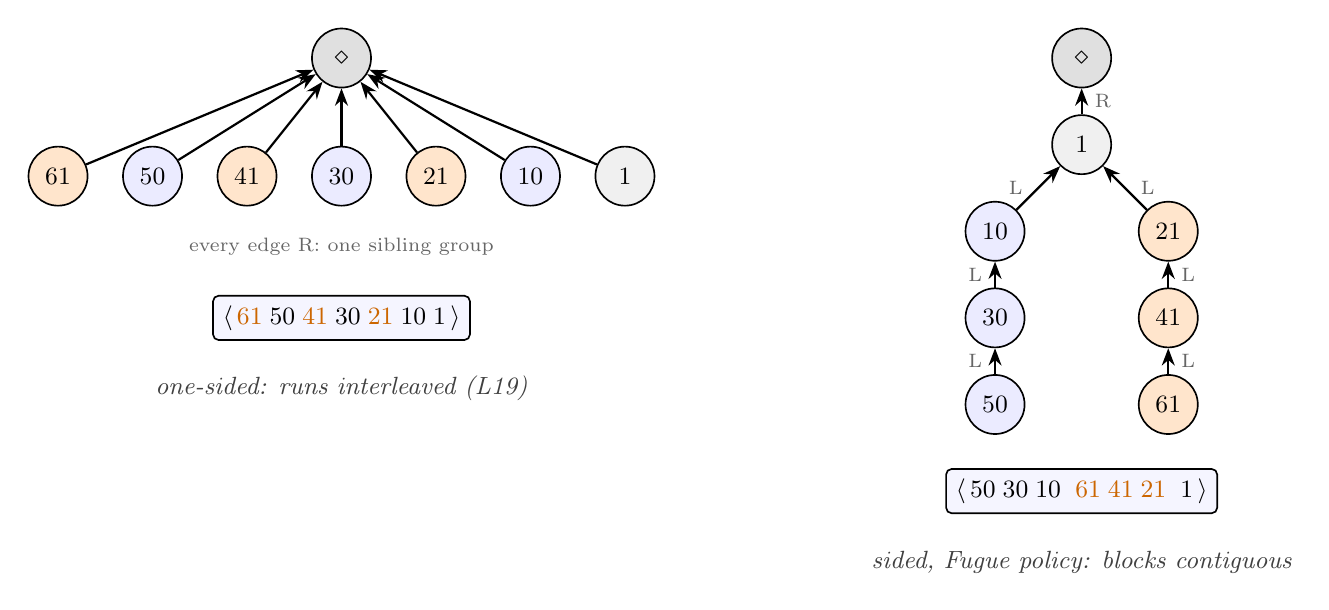
\begin{tikzpicture}
  % ---- left: one-sided (all-R), the L19 sibling fan
  \node[rootvtx] (fr) at (0,0) {$\diamond$};
  \node[vtx, fill=orange!20] (f61) at (-3.6,-1.5) {\small$61$};
  \node[vtx]                 (f50) at (-2.4,-1.5) {\small$50$};
  \node[vtx, fill=orange!20] (f41) at (-1.2,-1.5) {\small$41$};
  \node[vtx]                 (f30) at ( 0.0,-1.5) {\small$30$};
  \node[vtx, fill=orange!20] (f21) at ( 1.2,-1.5) {\small$21$};
  \node[vtx]                 (f10) at ( 2.4,-1.5) {\small$10$};
  \node[vtx, fill=black!6]   (f1)  at ( 3.6,-1.5) {\small$1$};
  \foreach \n in {f61,f50,f41,f30,f21,f10,f1}
    \draw[anc] (\n) -- (fr);
  \node[elbl] at (0,-2.4) {every edge R: one sibling group};
  \node[stbox] at (0,-3.3)
    {$\langle\,\textcolor{orange!80!black}{61}\;50\;
      \textcolor{orange!80!black}{41}\;30\;
      \textcolor{orange!80!black}{21}\;10\;1\,\rangle$};
  \node[capt] at (0,-4.2) {one-sided: runs interleaved (L19)};
  % ---- right: sided under the Fugue policy, backward runs = L-chains
  \begin{scope}[shift={(9.4,0)}]
  \node[rootvtx] (sr) at (0,0) {$\diamond$};
  \node[vtx, fill=black!6] (s1) at (0,-1.1) {\small$1$};
  \node[vtx]                 (s10) at (-1.1,-2.2) {\small$10$};
  \node[vtx, fill=orange!20] (s21) at ( 1.1,-2.2) {\small$21$};
  \node[vtx]                 (s30) at (-1.1,-3.3) {\small$30$};
  \node[vtx, fill=orange!20] (s41) at ( 1.1,-3.3) {\small$41$};
  \node[vtx]                 (s50) at (-1.1,-4.4) {\small$50$};
  \node[vtx, fill=orange!20] (s61) at ( 1.1,-4.4) {\small$61$};
  \draw[anc] (s1)  -- (sr) node[elbl, midway, right=1pt] {R};
  \draw[anc] (s10) -- (s1) node[elbl, midway, left=2pt]  {L};
  \draw[anc] (s21) -- (s1) node[elbl, midway, right=2pt] {L};
  \draw[anc] (s30) -- (s10) node[elbl, midway, left=1pt]  {L};
  \draw[anc] (s41) -- (s21) node[elbl, midway, right=1pt] {L};
  \draw[anc] (s50) -- (s30) node[elbl, midway, left=1pt]  {L};
  \draw[anc] (s61) -- (s41) node[elbl, midway, right=1pt] {L};
  \node[stbox] at (0,-5.5)
    {$\langle\,50\;30\;10\;\;
      \textcolor{orange!80!black}{61\;41\;21}\;\;1\,\rangle$};
  \node[capt] at (0,-6.4) {sided, Fugue policy: blocks contiguous};
  \end{scope}
\end{tikzpicture}
\caption{L19 under the two anchoring rules, the battery's own trace.
LCA document $\langle 1\rangle$; replica A (blue) types backward
$10, 30, 50$ before the head while replica B (orange) concurrently
types backward $21, 41, 61$. One-sided (left): every insert-before
anchors at the same left neighbor $\diamond$, both runs land in one
R-sibling group, and the timestamp-sorted fan interleaves them. Sided
under the Fugue policy (right): insert-before anchors at the
\emph{successor} as an L-entry, each run is an L-chain hanging off
$1$, and the in-order read keeps the blocks contiguous: L-extensions
precede the node ($50, 30, 10$ before their parents' line ending at
$1$), and among the L-siblings $10, 21$ of node $1$ the older run
displays first (the L band is mirrored). Both display strips are
machine outputs of \code{embed\_sided.py}.}
\label{fig:sided-l19}
\end{figure}

\paragraph{How the encoding realizes it, for zero extra bits.} The
one-sided block of \S\ref{sec:encoding} spends a constant leading
\code{1} per level whose only job is keeping coordinates nonempty;
repurpose it as the side bit. The L band needs an
order-\emph{reversing} prefix-free code, and the bit complement
$\overline{C}$ is exactly that at identical lengths (flipping every
bit flips every first-difference verdict and preserves both lengths
and prefix relations), so the block becomes
\[
  \mathrm{block}(\mathrm{side}, \delta) \;=\; \mathrm{sideBit}
  \,\|\, \bigl(C(\delta) \text{ if } R,\ \overline{C(\delta)}
  \text{ if } L\bigr),
\]
prefix-free per band, with no framing change and no new bits. On the
example, with the binary delta code ($C(1) = \code{0}$, $C(9) =
\code{1110001}$, $C(20) = \code{111100100}$, so $\overline{C(9)} =
\code{0001110}$, $\overline{C(20)} = \code{000011011}$), the stored
coordinates are the concatenated blocks:
\begin{center}\small
\begin{tabular}{@{}lll@{}}
\toprule
node & chain & stored coordinate (side bits marked) \\
\midrule
$1$  & $(R,1)$ &
  $\underline{\code{1}}\code{0}$ \\
$10$ & $(R,1)(L,9)$ &
  $\underline{\code{1}}\code{0}\;\underline{\code{0}}\code{0001110}$ \\
$21$ & $(R,1)(L,20)$ &
  $\underline{\code{1}}\code{0}\;\underline{\code{0}}\code{000011011}$ \\
$30$ & $(R,1)(L,9)(L,20)$ &
  $\underline{\code{1}}\code{0}\;\underline{\code{0}}\code{0001110}\;
   \underline{\code{0}}\code{000011011}$ \\
$50$ & $(R,1)(L,9)(L,20)(L,20)$ &
  $\underline{\code{1}}\code{0}\;\underline{\code{0}}\code{0001110}\;
   \underline{\code{0}}\code{000011011}\;
   \underline{\code{0}}\code{000011011}$ \\
\bottomrule
\end{tabular}
\end{center}
To compare two coordinates, parse: read a side bit; if \code{1},
decode one $C$ codeword as an R-band symbol $(R,\delta)$; if \code{0},
decode one $\overline{C}$ codeword (decode $C$ on the flipped bits) as
an L-band symbol $(L,\delta)$; repeat, then terminate with the marker.
Prefix-freedom per band delimits every block, so no length fields or
framing are needed, exactly as one-sided. The complement is what makes
the mirror free: within the L band, plain descending comparison of the
\emph{stored} bits is already the mirrored delta order ($
\overline{C(20)} = \code{000011011} < \overline{C(9)} = \code{0001110}
$ bitwise, matching $(L,20) < (L,9)$), so the carrier stores entropy
payload only and the marker-lex of the previous paragraph is read off
the bits. Faithfulness of this parse (unique decodability plus order
embedding of the sided alphabet) is machine-checked by the
chain-model/code-model lockstep below.

Two honest cost notes. Runs absorb the side bit like every other
run-constant (paid once at the head). On \emph{this} trace the sided
coordinates are longer than the one-sided fan's (the runs' deltas are
$20$ because the two replicas' Lamport clocks interleave); the
compression claim is about the common case, continuation-stamped
backward typing ($\delta = 1$ per keystroke, an \code{0}$\|
\overline{C(1)} = \code{01}$ block per level), where today's design
pays a growing-$\delta$ fan. Two-sidedness buys the semantics always
and the compression exactly when backward runs are locally stamped.

\paragraph{Side selection is a generation policy, not a datatype
choice.} If insert merely ``takes a side,'' convergence and
RA-linearizability hold for any sides whatsoever: those proofs never
consult the order's intent. What depends on \emph{which} side is
picked is the ordering intent. Fugue's non-interleaving needs the rule
``right child of the left neighbor when it has no right children, else
left child of the successor,'' and that rule lives at generation time,
where the framework already has a slot: honesty, the same layer that
polices the mint. The architecture is therefore one sided datatype,
verified once, policy-free (canonicity, fold exactness, the Join,
RA-linearizability), with intent theorems per generation policy: under
always-R, read-equivalence to the published RGA (the fragment theorem
composed with the compaction theorem); under the Fugue rule,
non-interleaving (a subtree is an in-order interval). RGA and Fugue
become two disciplines over one kernel rather than two datatypes.

\paragraph{Validation.} \code{whiteboard/litmus/embed\_sided.py}: the
chain semantics and the bit carrier as lockstep twin models, both run
under both policies. Every design prediction survived the first full
run:

\begin{center}\small
\begin{tabular}{@{}ll@{}}
\toprule
check & verdict \\
\midrule
full gauntlet under the Fugue policy (L1--L25, credential & clean,
  \textbf{including L19} \\
\quad family, subordination CEs, stale forks) &
  (out $= \langle 50,30,10,61,41,21,1\rangle$) \\
same gauntlet under always-R & clean except L19: the \\
 & one-sided fan, reproduced \\
chain semantics $\sim$ bit carrier, both policies & lockstep-EXACT
  (unique \\
 & decodability + order embedding) \\
all-R fragment $\sim$ the one-sided embed model & lockstep-EXACT, every
  scenario \\
randomized version-DAG PBT, all four models & 120 + 300 clean \\
\bottomrule
\end{tabular}
\end{center}

\noindent The Lean mechanization of both layers (the sided chain-lex
kernel and the sided conditioned instance, capstone included) has
landed kernel-clean; \S\ref{sec:mechanization} records it.

\section{Comparison with Eg-walker}
\label{sec:egwalker}

Eg-walker (Gentle \& Kleppmann, EuroSys 2025) is the closest system in
spirit, and the two designs can be read as the \emph{operational} and
\emph{denotational} realizations of one thesis, \textbf{pay for
concurrency, not for history}:

\begin{center}\small
\begin{tabular}{@{}p{0.31\textwidth}p{0.31\textwidth}p{0.31\textwidth}@{}}
\toprule
 & Eg-walker & embedded-chain RGA \\
\midrule
model & op-based; replicas exchange events & MRDT: three-way merge
  with an LCA \\
durable state & \textbf{full event graph on disk}, deletes included,
  retained while concurrent ops may arrive; document state
  metadata-free & \textbf{live nodes only}; no event log anywhere;
  dead survive as $\Theta(\log\delta)$ bits inside live coordinates \\
merge mechanism & \emph{replay}: walk the event graph, rebuild a
  transient CRDT structure (tombstones reappear transiently), discard
  at causally-linear points & \emph{refold}: $O(\text{survivors})$
  coordinate recomputation; no replay, no transient structure, no
  order decisions \\
sequential-editing cost & $\approx$ zero (plain edits; no metadata) &
  $\approx$ zero order metadata ($\sim$4 bits/level for continuation
  typing; a cursor jump pays log-gap once, at the run head) \\
concurrency cost & replay time proportional to the concurrent region,
  at every affected merge & coordinate bits proportional to
  $\log(\text{ts gap})$, once, in space \\
ordering semantics & Yjs-variant (FugueMax-adjacent); maximal
  non-interleaving \emph{conjectured}, not proved; two-sided (no L19
  analogue) & $\equiv$ published RGA (machine lockstep); one-sided:
  L19 backward-run interleaving inherited; removed by the sided
  generalization (\S\ref{sec:sided}), RGA kept as the all-R
  fragment \\
correctness artifact & informal proof (Appendix C) + property testing
  & L1--L25 battery + DAG PBT + lockstep vs RGA$_\dagger$;
  \textbf{RA-linearizability kernel-checked in Lean}
  (\S\ref{sec:mechanization}); the design was
  chosen so the merge proves itself (no order decisions to verify) \\
op payload & integer origin positions (compact, human-meaningful) &
  two timestamps + ghost prefix (droppable on the wire;
  \S\ref{sec:prefix}) \\
\bottomrule
\end{tabular}
\end{center}

\noindent Four sentences of honest positioning. \emph{(i)} Eg-walker
achieves its clean document state by keeping the entire history and
re-deriving order on demand; the embedded-chain RGA achieves it by
making order derivation unnecessary: the sort keys are written at
birth and never edited, and the coordinates are their encoding
(\S\ref{sec:encoding}), precomputed at mint time and exact forever.
\emph{(ii)} Eg-walker's ordering target was stronger where L19 is
concerned (Fugue-style two-sidedness removes backward interleaving,
while the one-sided design inherits RGA's anomaly by construction,
being read-equal to RGA); the sided generalization of
\S\ref{sec:sided} adopts exactly that two-sidedness as a parameter,
closing the gap while keeping the one-sided datatype as its all-R
fragment. \emph{(iii)} The verification gap runs
the other way: Eg-walker's replay-transform-clear loop is
algorithmically sophisticated and only informally proved; here the
merge performs no arbitration at all, the metatheory is one-line at
the chain layer plus a single faithfulness theorem at the encoding
layer, and RA-linearizability is a kernel-checked theorem in a
framework that had already verified a dozen-plus replicated
datatypes end-to-end (\S\ref{sec:mechanization}). \emph{(iv)} The
cost models part company at cursor jumps: a single-user history that
hops back to type at an old anchor is free for Eg-walker (nothing
concurrent to replay) but mints log-gap bits here, once per jump, at
the run head; on measured single-user editing traces the jump tail
is thin (code bits $\approx 1.4$--$1.8$ per level; see the companion
note of \S\ref{sec:encoding}). In the MRDT setting there is also a model
fit: Eg-walker must reconstruct merge context by replay because the
op-based model gives it none; the MRDT model hands the merge its LCA,
which is exactly the context replay rebuilds.

\section{Related work}
\label{sec:related}

The verified sweep of nearby systems lives in
\code{whiteboard/litmus/related-work.md} (per-claim verdicts, primary
sources); this section positions the datatype.

\paragraph{Retention taxonomy.} What nearby systems keep for the dead:
tombstone records (RGA with cemetery under causal stability; WOOT;
Yjs's per-deletion GC structs, kept forever; Fugue, ``we cannot
remove a deleted element's node entirely''; Peritext, ``the
positions must be remembered''); the full history (Eg-walker's event
graph, Chronofold/causal trees where the log \emph{is} the text);
consensus-gated compaction (Treedoc's flatten requires Paxos-commit);
or \textbf{dead identifiers inside live position keys} (Logoot/LSEQ,
Weidner's position-strings/list-positions, the Fugue id space). The
embedded-chain RGA is in the last class \emph{by information content}
(dead ancestors' timestamps persist inside survivors' sort keys,
at live-reachable scope), but with three deltas to its classmates:
the retention is \emph{delta-coded at the entropy of the anchor
gaps} (a sequential
history costs a constant per element where Logoot-family keys grow
with allocation policy), the \emph{birth tree kept whole} gives
forward non-interleaving and delete-order preservation (position-key
designs interleave, the PaPoC'19 anomaly, and Figma-style
fractional indexing is unsound under concurrency by its own account),
and the semantics is pinned to the best-studied sequence CRDT by a
machine-checked lockstep rather than being a new point in anomaly
space.

\paragraph{The impossibility backdrop.} Attiya et al.\ (PODC 2016)
prove $\Omega(D)$ metadata for push-based protocols meeting even the
weak list spec: the published form of ``ordering requires
remembering the dead.'' This design does not escape the bound; it
\emph{relocates and minimizes} the memory: $\Theta(\log \delta)$ bits
per dead-chain element inside live coordinates (plus the MRDT version
store, which the model provides). The sharper, machine-witnessed
form from our design sweep is the \emph{conservation law}
(\S\ref{sec:design}):
the sort key must retain dead ancestors' timestamps (the verdict
information survives every encoding change: stamp, spine, tombstone,
or denominator bits), and ties force separate \emph{metadata} only
under timestamp-oblivious minting; the timestamp-faithful mint carries
the same bits inside the coordinate. Eight timestamp-oblivious
mutation variants each have a named machine-checked countermodel
(fold-verdict erasure; repair non-locality); the credential
countermodel separates this design from all of them.

\paragraph{Verified datatypes.} Isabelle RGA (Gomes et al.\ OOPSLA'17,
op-based convergence), OpSets (list semantics specified by a total
order of identified ops: arbitration-by-identity as specification),
VeriFx (SMT, convergence properties), MET (TLA+, list CRDT bugs). In
the MRDT line (Kaki et al.\ OOPSLA'19; Peepul PLDI'22; RA-lin
OOPSLA'25, this framework), no verified sequence with
sequence-CRDT-grade ordering guarantees existed; our verified rehoming
RGA (\S\ref{sec:design}) is RA-linearizable against its own fold yet
fails the sequential delete-order spec, since RA-linearizability
certifies convergence to the datatype's \emph{own} semantics and
ordering intent must be specified and proved separately. The
embedded-chain RGA delivers the missing artifact:
RA-linearizability is a kernel-checked Lean theorem
(\S\ref{sec:mechanization}); delete-order preservation, display
stability and forward non-interleaving are proved at the model layer;
and the RGA read-equivalence (the compaction theorem,
\S\ref{sec:mechanization}) closes the intent question against the
best-studied sequence semantics.

\paragraph{Treedoc's lesson, inverted.} Treedoc re-balances geometry
and must pay consensus for it; the principle that emerged from our
ledger-based sibling design study
(\emph{reprojection without consensus is safe iff geometry has been
demoted to a rendering}) is here taken to its fixed point: geometry is
never reprojected at all. It is immutable, so it may safely be the
only thing.

\section{Mechanization: the conditioned discharge and the compaction
theorem}
\label{sec:mechanization}

The verification framework is Part~I's metatheory; file paths below
are relative to the Sal repository.

\textbf{The capstone is proved} (2026-07-15, kernel-clean on
$\{\mathrm{propext}, \mathrm{Classical.choice},
\mathrm{Quot.sound}\}$):
\[
  \code{embed\_ra\_linearizable3} \;:\;
  \mathrm{EReach}\ \Gamma\ C \to \mathrm{IsRALinearizable3}\ C
\]
i.e.\ RA-linearizability per version at every honestly reachable
configuration, \emph{parametric in the code} $\Gamma$: the unary
code, the binary delta code, and the flipped Elias-$\delta$ code are
all proved \code{OrderedPrefixCode} instances, three encodings on
one proof. The factoring is exactly this
part's design--encoding split, which is itself evidence for the split:

\begin{enumerate}
\item \textbf{Model layer} (\code{Sal/MRDTs/RGA\_Embed/}, six
files, 0 sorry, plus the read-equivalence order core and the sided
kernel noted below): the code-parametric kernel; commutations \emph{to
state equality} under $\rcrel = \Either$ (\code{rc\_non\_comm'});
\code{ins\_prefix\_ghost}; coherence and chain-generation closures;
display stability, with step stability (S2, delete-order preservation at
its \code{del} instance) proved \emph{without any axioms} and merge pairwise
stability (S4, the adopted contract); unique decodability
(\code{coordOf\_inj}); \textbf{the chain-lex theorem}
(\code{display\_iff\_chainBefore} = Corollary~\ref{cor:lex});
non-interleaving as subtree convexity (\code{subtree\_convex});
Theorem~\ref{thm:faithful}(i) for all three codes
(\code{binEnc\_mono}/\code{binEnc\_prefixFree},
\code{dEnc\_mono}/\code{dEnc\_prefixFree}, cross-validated
against the Python codes by kernel \code{decide});
\code{native\_decide} SPOTs where the rehoming RGA's delete-reorder
witness gets the opposite verdict.
\item \textbf{Conditioned instance}
(\code{Sal/ConditionedMRDTs/MRDT\_Instances/EmbedRGA/}, nine
sections, 0 sorry, plus the Elias-$\delta$ inheritance corollary
\code{EmbedRGA\_EliasDelta.lean}), proved via the \emph{mergeable-queue
route} of \S\ref{sec:route}: a
generic join lemma (\code{JoinLemma3At}: the merge exhibits its own
linearization witness) plus an honest-reachability metatheorem
(\code{HonestReach}), rather than the rehoming RGA's 55-file bespoke
chain. The route applies exactly when states are canonical per event
set, which is Theorem~\ref{thm:chain}(i).
Landed: the canonical sorted-list state; strictly-sorted
extensionality (\code{esorted\_ext}: sorted lists with the same
members are equal, replacing any canonical-list formula);
\textbf{fold-canonicity} (\code{e\_fold\_canon}: well-formed
enumerations of one event set fold to the \emph{same} state;
Theorem~\ref{thm:chain}(i) mechanized); the honesty core and its
bridge to well-formedness; the merge membership characterization
(\code{e\_mergeL\_mem}, OR-set survival with honesty closing the
cross-branch-delete corner); the Join (\code{e\_join\_at}: the
merge is its own linearization witness); the capstone; the honesty
discharge from the framework's generation discipline
(\code{eHonest\_of\_applicable}: applicable generation forces the
honesty core, so per-op honesty needs no bespoke oracle); and the
instance intent theorems: delete-order preservation \emph{is}
sublist stability (\code{eUpdate\_del\_sublist} is literally
\code{List.filter\_sublist}: a delete's successor state is a sublist
of its predecessor, so the surviving display order is untouched;
the merge preserves each input's survivor order on both sides).
\end{enumerate}

\noindent\textbf{The compaction theorem is proved} (2026-07-15,
kernel-clean): $\mathrm{read} \circ \mathrm{embed} = \mathrm{read}
\circ \mathrm{RGA}_\dagger$ on honest executions, as
\code{rga\_read\_eq\_embed\_read}
(\code{EmbedRGA\_ReadEquiv.lean}): for every well-formed enumeration
of an honest event set, \emph{any} enumeration of the tombstoned
fold's visible ids in the published RGA's own relational order
(\code{visible\_lt}) equals the embed fold's id sequence, with
element agreement (\code{embed\_rec\_readSeq}). The proof is
\emph{against the published definition}: the order core
(\code{Sal/MRDTs/RGA\_Embed/RGA\_Embed\_ReadEquiv.lean}) shows
\code{visible\_lt} coincides with chain-lex on the shared birth tree
(soundness by induction on derivations, completeness by realizing
every chain prefix as an \code{afters}-reachable ancestor), and en
route proves the published relational order total and asymmetric on
the birth tree, facts the published side never had. This converts
the design into a theorem \emph{about} the published RGA: it admits a
strictly-live compaction preserving every read. The lockstep rows of
\S\ref{sec:validation} are this theorem's tested form.

\medskip
\noindent\textbf{The sequential specification is proved, and the
design holds the canonical seat} (2026-07-16). The campaign of
Part~III proved \code{embed\_seq\_sound}: on every sequentially honest
single-replica history the canonical sorted state is the naive
insert-at-position text buffer, record for record, with the adjacency
lemma (\code{chainBefore\_snoc\_iff}: a fresh insert's delta beats
every existing child's by sum-telescoping) as the geometric heart
(\S\ref{sec:tiers}). The published RGA$_\dagger$ inherits the same
buffer spec through the compaction theorem
(\code{rga\_seq\_read\_eq\_buffer}), and the same statement is refuted
for the rehoming design (\S\ref{sec:refuted}), which demoted it
repo-wide: the embedded-chain family is the repository's canonical
sequence RDT, and the canonical fused Peritext was re-based onto this
kernel (\code{Peritext\_Embed/}: capstone by pure instantiation of the
payload-generic instance; \code{renderIds\_del}, deleting a character
never re-formats another, the theorem the rehoming kernel provably
lacks; and the tier-4 editor theorem
\code{peritextEmbed\_seq\_sound}). One caveat is recorded as Open
Question~\ref{oq:seqwitness}: per-replica soundness and convergence do
not compose into ``the merged read is the naive buffer on some
ordering of the union''; the dead-anchor corner
(\S\ref{sec:caveat}) is where stamp-sorted replay diverges from the
fold.

\medskip
\noindent\textbf{The sided generalization is proved} (2026-07-15,
kernel-clean), in the same two layers as \S\ref{sec:sided} presents
it. The sided chain-lex kernel
(\code{Sal/MRDTs/RGA\_Embed/Sided\_ChainLex.lean}): the sided marker
theorem \code{sdisplay\_iff\_schainBefore} (display comparison of
sided coordinates IS the in-order rule), totality of the display
relation \emph{without any axioms}, unique decodability
(\code{sidedCoordOf\_inj}: the side is recoverable from the first
symbol's band, the delta by prefix-freedom within the band), the
all-R \emph{fragment theorem} \code{schainBefore\_liftR} (all-R chains
order exactly as one-sided chains: ``RGA is the all-R fragment,''
mechanized), and in-order-interval subtree convexity
(\code{schain\_subtree\_convex}, the datatype half of the L19
discharge). The conditioned instance
(\code{MRDT\_Instances/SidedRGA/}, nine sections mirroring the
one-sided instance with the sided key): fold-canonicity
(\code{s\_fold\_canon}), the Join by the same mergeable-queue route,
and the capstone
\[
  \code{sided\_embed\_ra\_linearizable3} \;:\;
  \mathrm{SReach}\ \Gamma\ C \to \mathrm{IsRALinearizable3}\ C
\]
\emph{for every side assignment}: sides are payload to convergence,
which is the policy/datatype split of \S\ref{sec:sided} as a theorem,
with \code{sHonest\_of\_applicable} discharging honesty from the
generation guard exactly as one-sided. The per-policy intent
theorems have since landed, and the policy story is a machine-checked
three-act arc (2026-07-16/17). \emph{Act one}: \code{sFold\_liftOp},
the all-R sided fold IS the one-sided fold, unconditionally (the sort
keys coincide definitionally), so every one-sided theorem transports;
and \code{sided\_fold\_subtree\_convex}, subtrees display as
contiguous blocks in any chain-generated fold, so runs that chain
never interleave (\code{fugue\_reachable\_runs\_no\_interleave}).
\emph{Act two}: the Weidner--Kleppmann maximal-non-interleaving
Definition~4 was formalized over reachable configurations
(\code{SidedRGA\_Fugue.lean}) and REFUTED twice for this Fugue
policy on reachable traces (the recency tiebreak reverses the paper's
lowest-ID-first; their Figure-7 execution): the paper's own
Fugue-vs-FugueMax separation, landing on this implementation.
\emph{Act three}: FugueMax realized as a kernel variant
(\code{SidedMax\_ChainLex.lean}): its sibling order depends on the
right ORIGIN, not expressible by any re-banding of deltas (the mirror
control machine-witnesses this), so R-entries carry the mint-time
successor's key as an order-reversing tag; condition (3) is proved in
full (\code{fuguemax\_same\_origin\_low\_first}, the positive twin
of the refutation) and full Theorem~9 is reduced to the
display-to-traversal theory (task \#88; Open
Question~\ref{oq:traversal}). The sided
sequential spec also landed (\code{sided\_seq\_sound}: a
sentinel-rooted two-sided buffer, R-inserts splice after their
anchor, L-inserts immediately before). The tag has a COST: at
contested inserts the coordinate embeds the successor's key,
$\Theta(|\text{key}|)$ where plain Fugue pays zero, and whether that
retention is a lower bound for tombstone-free maximal
non-interleaving is an open question with a Myhill--Nerode shape
(task \#89; Open Question~\ref{oq:retention}): the entropy law of
\S\ref{sec:encoding} meeting the ordering intent.

\paragraph{Provenance.} \code{whiteboard/litmus/embed\_tree.py} (the
design, the timestamp-oblivious control, the credential countermodel,
the IEEE 754 measurements; \code{python3 embed\_tree.py} /
\code{fp} / \code{code}); \code{litmus.py}, \code{pbt.py} (battery and
DAG harness); \code{contest\_tree.py} (lockstep harness, CE
regressions); \code{whiteboard/retention-countermodel.pdf} (the
retention arc that forced this design);
\code{whiteboard/delta-tree-design.pdf} (the ledger-based sibling
design and the invariants I1--I3);
\code{whiteboard/litmus/related-work.md} (verified source list:
Roh et al.\ JPDC'11; Attiya et al.\ PODC'16; Kleppmann et al.\
PaPoC'19; Weidner \& Kleppmann TPDS'25 (Fugue); Gentle \& Kleppmann
EuroSys'25 (Eg-walker, arXiv:2409.14252); Preguiça et al.\ ICDCS'09
(Treedoc); Grishchenko \& Patrakeev PaPoC'20 (Chronofold); Litt et
al.\ CSCW'22 (Peritext); Gomes et al.\ OOPSLA'17; OpSets 2018; Kaki et
al.\ OOPSLA'19; Peepul PLDI'22; RA-lin OOPSLA'25; VeriFx ECOOP'23;
Figma/Wallace fractional indexing; Weidner position-strings).

%======================================================================
\part{Sequential specifications: convergence is not correctness}
%======================================================================

\noindent
Replication-aware linearizability certifies that every version of a
replicated data type is the fold of some delivery-respecting
linearization of its events. The reference point of that guarantee is
the datatype's \emph{own} fold: a bug in \code{do} appears identically
on every replica, converges perfectly, and passes every convergence
theorem. This part records the campaign that closes the gap. For every
production RDT in Sal there is now a kernel-checked theorem that the
fold of any single-replica history equals the output of a
straightforward sequential program, the one a programmer would write
with no replication in mind. The campaign's unifying observation is
the \emph{witness discipline}: sequential interfaces address state
positionally (\code{dequeue()} is nullary, \code{insert} names an
index), replicated operations cannot, and every replicated operation
therefore carries the identity of what its issuer \emph{observed} the
positional referent to be; the honesty side conditions of the theorems
are exactly the faithfulness of those witnesses. The campaign's
negative results carry as much information as its theorems: the
rehoming tombstone-free RGA is refuted at this specification on a
four-op single-replica trace, its fused Peritext inherits the
refutation at the render, and Shesha passes sequentially while failing
at the merge, so do-faithfulness and merge-faithfulness are
independent axes, and both separations are kernel-checked. A final
section states what the campaign does \emph{not} give: per-replica
soundness and convergence do not compose into ``the merged state is
some user's sequential result,'' and the precise corner where
composition fails is the dead-anchor corner the sequence-CRDT
trilemma names. Every claim below names its Lean identifier.

\section{The specification gap}
\label{sec:gap}

The framework's central guarantee is RA-linearizability at every
reachable configuration: each version the store registers is
$\mathrm{fold}(\rho)$ for some enumeration $\rho$ of the version's
event set that respects delivery order. This is the right guarantee
for \emph{replication}: the merge invented nothing, reordered nothing
it was not entitled to reorder, and all replicas agree.

It says nothing about whether the fold is \emph{right}. The reference
sequence is the datatype's own \code{do}; if \code{do} is wrong, every
replica is wrong in unison (Figure~\ref{fig:loop}). Two incidents made
this concrete in this repository. First, a mark-extent defect in an
early Peritext render passed every convergence obligation and was
caught only by eye. Second, and decisively: the rehoming tombstone-free
RGA carries a fully general, kernel-clean RA-linearizability capstone
(\code{rga\_ra\_linearizable3\_eq}), and its \code{do} nonetheless
reorders surviving text when an interior element is deleted, with no
concurrency anywhere in the history (\S\ref{sec:refuted}). Both
defects are invisible to convergence because convergence is
self-referential.

\begin{figure}[h]
\centering
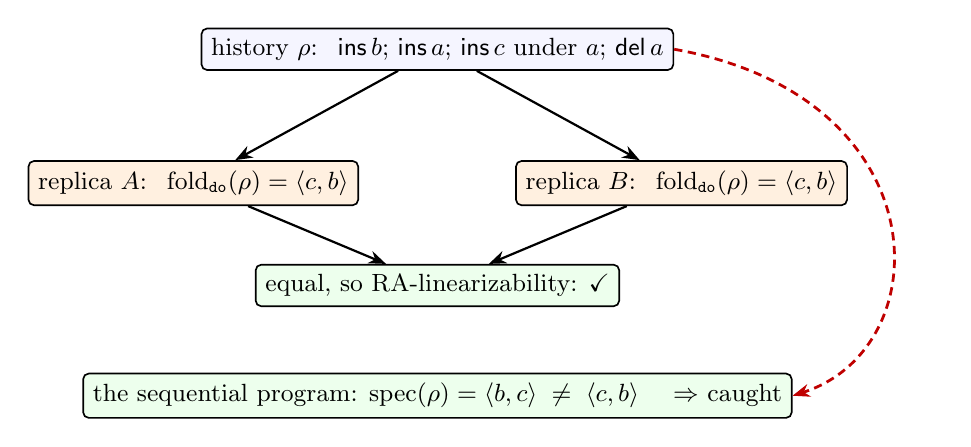
\begin{tikzpicture}
  \node[stbox] (ops) at (0,0)
    {history $\rho$: \ $\ins\,b$;\ $\ins\,a$;\ $\ins\,c$ under $a$;\ $\del\,a$};
  \node[badbox] (ra) at (-3.1,-1.7)
    {replica $A$: \ $\mathrm{fold}_{\code{do}}(\rho) = \langle c, b\rangle$};
  \node[badbox] (rb) at (3.1,-1.7)
    {replica $B$: \ $\mathrm{fold}_{\code{do}}(\rho) = \langle c, b\rangle$};
  \draw[anc] (ops) -- (ra);
  \draw[anc] (ops) -- (rb);
  \node[okbox] (conv) at (0,-3.0)
    {equal, so RA-linearizability: $\checkmark$};
  \draw[anc] (ra) -- (conv);
  \draw[anc] (rb) -- (conv);
  \node[stbox, fill=green!7] (spec) at (0,-4.4)
    {the sequential program: $\mathrm{spec}(\rho) = \langle b, c\rangle
     \;\neq\; \langle c, b\rangle$ \quad $\Rightarrow$ caught};
  \draw[wit] (ops.east) .. controls (6.4,-0.6) and (6.4,-3.8) .. (spec.east);
\end{tikzpicture}
\caption{Why convergence cannot see a \code{do} bug. A defective fold
is applied identically everywhere, so all replicas agree and every
convergence theorem passes over the shared mistake. Only a reference
computed by something \emph{other than} \code{do} (dashed) can
disagree. The history shown is the real refutation trace of
\S\ref{sec:refuted}.}
\label{fig:loop}
\end{figure}

The remedy is an independent specification. For sequential behaviour
there is a canonical one: \emph{the sequential program a programmer
would write for the same operations with no replication in mind}. A
counter is addition. A queue is a list. A text buffer is
insert-at-position and delete. A marked-text editor is a buffer of
characters and boundary tokens with one left-to-right walk.

\section{The obligation, and the rules of engagement}
\label{sec:obligation}

The campaign's obligation, per datatype:
\begin{center}
\begin{tabular}{c}
\emph{for every sequentially honest single-replica history $\rho$:}\\[3pt]
$\mathrm{read}(\mathrm{fold}(\rho)) \;=\; \mathrm{spec}(\rho)$
\end{tabular}
\end{center}
proved by discovering an inductive invariant of the fold, never by
weakening the spec to match the implementation. ``Sequentially
honest'' is the datatype's own issuing discipline specialized to a
linear history (fresh, monotone stamps; each operation applicable at
the state it executes against), so the theorems attack no strawman:
the histories quantified over are exactly the ones a single
well-behaved replica produces, and in every case the side condition
reuses a contract the convergence proofs already consume.

Three method rules were fixed in advance and held throughout.
\emph{Falsifiable statement first}: each tier states its equality
before proof work begins, and a refutation is a first-class outcome
(three landed, \S\ref{sec:refuted}). \emph{The spec is external}: the
sequential program is written from the datatype's user-facing intent,
never read off the implementation; where the two disagree, the
disagreement is the result. \emph{Tests carry both polarities}: every
concrete test block pairs its expected values (hand-derived, never
evaluated out of the code under test) with should-fail companions, so
the harness demonstrably discriminates; the refutation files pair each
negative with the positive prefix on which the two sides still agree,
isolating the departing operation exactly.

\section{The observation gap: positional interfaces, witnessed ops}
\label{sec:witness}

Writing out the specifications exposes one structural pattern, and it
is the campaign's most instructive artifact. A sequential structure
addresses its state \emph{positionally or implicitly}:
\code{dequeue()} takes no argument because ``the head'' is
unambiguous; \code{insert(i, e)} names an index; \code{write(v)}
implicitly overwrites everything before it. A replicated datatype can
afford none of this, because positions and implicit referents are not
stable under concurrent edits: by the time an operation is applied
elsewhere, ``the head'' may be a different element and index $i$ a
different character. So the replicated operation carries a
\textbf{witness}: the identity (tag, stamp, id, coordinate, snapshot)
of what the issuing replica \emph{observed} the positional referent to
be, at its own state, at issue time (Figure~\ref{fig:witness-queue}).

\begin{figure}[h]
\centering
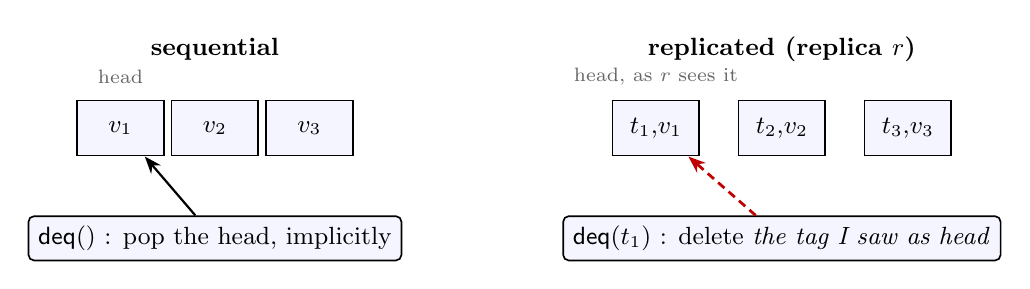
\begin{tikzpicture}
  % left: sequential
  \node[font=\small\bfseries] at (0,1.0) {sequential};
  \node[cell] (s1) at (-1.2,0) {$v_1$};
  \node[cell] (s2) at (0,0)    {$v_2$};
  \node[cell] (s3) at (1.2,0)  {$v_3$};
  \node[elbl] at (-1.2,0.65) {head};
  \node[stbox] (sop) at (0,-1.4) {$\deq()$ : pop the head, implicitly};
  \draw[anc] (sop) -- (s1);
  % right: replicated
  \begin{scope}[shift={(7.2,0)}]
  \node[font=\small\bfseries] at (0,1.0) {replicated (replica $r$)};
  \node[cell] (t1) at (-1.6,0) {$t_1{,}v_1$};
  \node[cell] (t2) at (0,0)    {$t_2{,}v_2$};
  \node[cell] (t3) at (1.6,0)  {$t_3{,}v_3$};
  \node[elbl] at (-1.6,0.65) {head, as $r$ sees it};
  \node[stbox] (rop) at (0,-1.4)
    {$\deq(t_1)$ : delete \emph{the tag I saw as head}};
  \draw[wit] (rop) -- (t1);
  \end{scope}
\end{tikzpicture}
\caption{The observation gap, on the queue. The sequential
\code{dequeue} is nullary; the replicated one names the tag its issuer
read as the head of its own replica (dashed: the witness). Honesty is
the faithfulness of the witness: \code{qOK} states that the fold at
the issue point is literally $(t_1, v_1) :: \mathit{rest}$.}
\label{fig:witness-queue}
\end{figure}

The sequential-honesty side conditions of \S\ref{sec:obligation} are
then exactly the statement \emph{the witness is what the sequential
operation would have seen}, and each campaign theorem says: under that
discipline, the witnessed-identity program implements the positional
program. Where no witness is needed the alphabets coincide and the
spec is a view homomorphism. The whole catalogue of
\S\ref{sec:specs} sorts by this principle, and the summary is one
sentence: \emph{every honesty condition in the campaign is the
faithfulness of a witness that replaced a positional argument.}

\section{The specifications, datatype by datatype}
\label{sec:specs}

\subsection{No gap: the alphabets already coincide}

For nine of the flat datatypes the RDT operation is literally the
sequential operation; the state carries invisible bookkeeping (tags,
per-replica slots) and the spec is the evident program on the
user-visible view.

\begin{itemize}
\item \textbf{Counter, increment-only counter.} Spec state
  $\mathbb{Z}$ (resp.\ $\mathbb{N}$); increment is $n \mapsto n + 1$.
  The fold \emph{is} the history length
  (\code{counter\_seq\_sound}, \code{ioc\_seq\_sound}).
\item \textbf{PN-counter.} Spec: $\#\mathsf{inc} - \#\mathsf{dec}$
  (\code{pnSpec}); \code{pn\_seq\_sound}.
\item \textbf{Grow-only set and map; conditioned G-set.} Spec:
  accumulation; $x$ is a member iff some operation added $x$
  (\code{goset\_seq\_sound}, \code{gomap\_seq\_sound},
  \code{gsetcond\_seq\_sound}).
\item \textbf{OR-set, plain and efficient.} Spec state: a plain set;
  $\mathsf{add}\,e$ inserts, $\mathsf{rem}\,e$ deletes
  (\code{orSpecStep}). The tag machinery (fresh $(t, e)$ stakes;
  remove filters every tag of $e$) is invisible to one replica: the
  element view of the fold is the naive program
  (\code{orset\_seq\_sound}, \code{orsete\_seq\_sound}), a fold
  homomorphism, no invariant needed.
\item \textbf{Enable-wins flag.} Spec state: one boolean;
  $\mathsf{enable} \mapsto \mathsf{true}$,
  $\mathsf{disable} \mapsto \mathsf{false}$ (\code{ewSpecStep});
  \code{ewflag\_seq\_sound}.
\item \textbf{Add-wins priority queue.} A two-part spec pins both
  state components: membership behaves as the plain add/remove set
  with $\mathsf{inc}$ inert (\code{awpqSpecStep},
  \code{awpq\_mem\_seq\_sound}), and the increment component is a
  grow-only log of exactly the issued increments
  (\code{awpq\_inc\_log\_sound}).
\end{itemize}

\subsection{Gap: arbitration by stamp instead of program order}

\textbf{LWW and FWW registers.} The sequential register is
$\mathsf{write}\,v$ with \emph{program order} deciding who wins; the
spec programs are ``the last write's value'' (\code{lwwSpecFold}) and
``the first write's value'' (\code{fwwSpecFold}). The RDT operation
carries its Lamport stamp \emph{as the arbitration key in the payload}
(a max- resp.\ min-semilattice on stamped writes), because concurrent
replicas have no shared program order to appeal to. The gap is a
transfer of ordering authority from control flow to data, and the
honesty condition is precisely its repair: \code{stampsMono} (stamps
strictly increase along the history, the sequential Lamport
condition), under which the arbitration key agrees with program order
and \code{lww\_seq\_sound} / \code{fww\_seq\_sound} recover last- and
first-write semantics. Without \code{stampsMono} the statements are
false, and should be: a replica that back-dates a write is asking LWW
to disagree with program order.

\subsection{Gap: overwrite by snapshot instead of ``everything''}

\textbf{Multi-valued register.} The sequential $\mathsf{write}\,v$
implicitly overwrites everything before it. The RDT operation is
$\mathsf{write}\,(v, O)$ where $O$ is a \textbf{prepare-time
snapshot}: the write-stamps the issuer currently sees, named
explicitly so that a \emph{concurrent} write (absent from $O$)
survives, which is the point of an MVR. The sequential spec is still
the plain last-write register (\code{mvrSpecFold}). Honesty
(\code{mvrOK}): the stamp is fresh and $O$ lists \emph{exactly} the
issuer's visible stamps, the formal form of ``I overwrite precisely
what I can see.'' Under it, \code{mvr\_seq\_sound}: the visible-value
view of the fold is the last write. The proof needs the campaign's
first genuinely discovered invariant, \code{mvr\_over\_tags}: every
overwritten stamp was staked, which is what makes a fresh stamp
provably not-yet-overwritten.

\subsection{Gap: dequeue() becomes delete-what-I-saw}
\label{sec:queue}

\textbf{The mergeable queue}, the cleanest specimen
(Figure~\ref{fig:witness-queue}). The sequential queue is
\[
  \enq\,v : S \mapsto S \mathbin{+\!\!+} [v]
  \qquad\qquad
  \deq() : S \mapsto \mathrm{tail}(S).
\]
The RDT operation is $\deq\,t$: remove \emph{by tag}, $t$ being the
tag of the element the issuing replica read as the head of its own
queue; the implementation filters $t$ out of the whole list, wherever
it sits. The spec keeps the sequential shape, \code{tail}, blind to
$t$ (\code{qSpecStep}). Honesty (\code{qOK}) is witness faithfulness:
the fold at the issue point is literally $(t, v) :: \mathit{rest}$.
The invariant \code{q\_tags\_nodup} (fresh stakes stay duplicate-free)
makes filter-by-tag remove exactly the head, and
\code{queue\_seq\_sound} closes the loop: delete-what-I-saw implements
pop-the-head. Its axiom audit is the leanest in the campaign:
$\{\mathrm{propext}, \mathrm{Quot.sound}\}$, no choice anywhere. The
same witness discipline is what the convergence side already consumed
(\code{qHonest\_of\_applicable}); nothing was invented for the
occasion.

\subsection{Gap: insert-at-index becomes insert-after-who-I-saw}
\label{sec:rga-spec}

\textbf{The embedded-chain RGA.} The sequential text buffer is
$\mathsf{insert}(i, e)$ and $\mathsf{delete}(i)$, index-addressed. The
RDT operation is $\ins(e, \pi, a)$: $a$ is the \emph{id} of the
element the issuer saw at position $i - 1$ (its anchor; the sentinel
$0$ for the head), and $\pi$ is the anchor's stored coordinate as the
issuer read it (the proof-carrying prefix); $\del(x)$ names the id
seen at position $i$. The spec program is the buffer in id-clothing
(\code{eSpecStep}): front-cons for $a = 0$, otherwise splice
immediately after $a$'s entry (\code{eInsAfter}); delete filters by
id. On a sequential history the anchor id determines the index
uniquely, so this \emph{is} the positional program with positions
named by their occupants. Honesty (\code{eSeqOK}): stamps exceed all
prior insert stamps, and each operation is applicable at the current
fold, i.e.\ the anchor is live and carries exactly $\pi$. The theorem
(\code{embed\_seq\_sound}, \S\ref{sec:tiers}) is the strongest form in
the campaign: the canonical sorted state equals the spec buffer
\emph{record for record}. The same spec, verbatim, is what the
rehoming RGA is refuted against (\S\ref{sec:refuted}); its gap is not
the witness (the rehoming op carries one too, plus a path) but the
implementation moving \emph{other} elements' referents on delete.

\subsection{Gap: one mark becomes a boundary pair}

\textbf{Fused Peritext.} The sequential marked-text editor has an
\emph{atomic} $\mathsf{mark}(i, j, m)$. The fused RDT has no such
operation: a mark is \textbf{two} ordinary inserts of boundary
elements $\langle m\rangle$ and $\langle/m\rangle$ sharing a fresh
mark id, anchored at the range ends; mark removal is two deletes. An
atomic positional operation is traded for a \emph{pair} of witnessed
inserts, which is the atomicity horn of the mark-positioning trilemma,
accepted knowingly. The spec therefore lives at the token level: the
editor is the \S\ref{sec:rga-spec} buffer over
$\mathrm{char} \oplus \mathrm{boundary}$ entries plus one
left-to-right walk maintaining the open-mark set (a start boundary
opens, the matching close removes, characters display with what is
open). \code{peritextEmbed\_seq\_sound} says the datatype's render is
that editor's screen, id for id in the \code{\_ids} variant; the
range-level reading is recovered by the positional intent theorems
(\code{render\_id\_active\_iff\_between}: a character carries mark $m$
iff it sits, in reading order, strictly between $m$'s boundaries).
The pair encoding is also why the character/boundary distinction is
load-bearing in the delete theorem: deleting a \emph{character}
re-formats nothing (\code{renderIds\_del}), while deleting a
\emph{boundary} is mark removal and must re-format its span
(machine-checked necessary: \code{boundary\_delete\_breaks\_filter\_eq}).

\section{The proofs: four tiers, three kinds of invariant}
\label{sec:tiers}

The campaign ran easiest to hardest, and the difficulty gradient
turned out to be a gradient of invariant \emph{kinds}.

\paragraph{Tier 1 (eleven flat datatypes), \code{SeqSpec\_Flat.lean}.}
Mostly view homomorphisms, no invariant at all. The two exceptions
need \emph{identity hygiene}: facts about tag bookkeeping that hold on
every reachable single-replica state and are exactly what the
induction consumes. For the MVR, \code{mvr\_over\_tags} (overwritten
stamps are staked); for the AWPQ, duplicate-freedom of stakes.

\paragraph{Tier 2 (the mergeable queue),
\code{MergeableQueue\_SeqSpec.lean}.}
One identity-hygiene invariant, \code{q\_tags\_nodup}, as described in
\S\ref{sec:queue}.

\paragraph{Tier 3 (the embedded-chain RGA),
\code{EmbedRGA\_SeqSpec.lean}.}
The invariant becomes \emph{geometric}. The spec splices an insert
immediately after its anchor; the datatype sorts records by
birth-chain coordinates; the bridge is the \textbf{adjacency lemma}
(\code{chainBefore\_snoc\_iff}, Figure~\ref{fig:adjacency}): a fresh
insert's chain $c_a \mathbin{+\!\!+} [\delta]$ sits directly after its
anchor's chain $c_a$ in display order, because the fresh timestamp gap
$\delta$ exceeds every delta any existing chain hangs off $c_a$, a
fact that costs only sum-telescoping (a chain's deltas sum to its id,
and every existing id is below the fresh stamp). The sorted canonical
state then \emph{is} the spec buffer, record for record
(\code{embed\_seq\_sound}). Two transports come for free. The
published tombstoned RGA is read-equivalent to the embed on honest
event sets (the compaction theorem, \S\ref{sec:mechanization}), so it
inherits the buffer spec:
\code{rga\_seq\_read\_eq\_buffer} and element-level
\code{rga\_seq\_read\_element} (\code{EmbedRGA\_SeqSpec\_RGA.lean}, a
standalone build target because the two RGA models share top-level
names). And the sided generalization simulates the one-sided instance
on all-R histories unconditionally (\code{sFold\_liftOp}), so the
buffer spec transports to the sided datatype's all-R fragment at zero
proof cost; the full two-sided theorem has since landed as
\code{sided\_seq\_sound} (\code{SidedRGA\_SeqSpec.lean}): a
sentinel-rooted buffer where an R-insert splices immediately after its
anchor and an L-insert immediately before it, via the two sided
adjacency lemmas (\code{schainBefore\_snocR\_iff},
\code{snocL\_iff}, axioms $\{\mathrm{propext},
\mathrm{Quot.sound}\}$).

\begin{figure}[h]
\centering
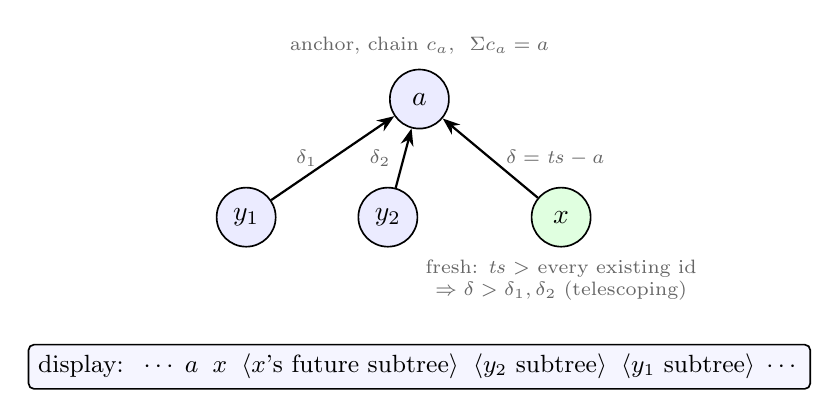
\begin{tikzpicture}
  \node[vtx] (a) at (0,0) {$a$};
  \node[elbl] at (0,0.68) {anchor, chain $c_a$, \ $\Sigma c_a = a$};
  \node[vtx] (c1) at (-2.2,-1.5) {$y_1$};
  \node[vtx] (c2) at (-0.4,-1.5) {$y_2$};
  \node[vtx, fill=green!12] (x) at (1.8,-1.5) {$x$};
  \draw[anc] (c1) -- (a) node[elbl, midway, left=2pt] {$\delta_1$};
  \draw[anc] (c2) -- (a) node[elbl, midway, left=1pt] {$\delta_2$};
  \draw[anc] (x) -- (a) node[elbl, midway, right=2pt]
    {$\delta = \mathit{ts} - a$};
  \node[elbl, align=center] at (1.8,-2.3)
    {fresh: $\mathit{ts} > $ every existing id\\
     $\Rightarrow \delta > \delta_1, \delta_2$ (telescoping)};
  \node[stbox] at (0,-3.4)
    {display: \ $\cdots\; a \;\; x \;\;
      \langle x\text{'s future subtree}\rangle \;\;
      \langle y_2 \text{ subtree}\rangle \;\;
      \langle y_1 \text{ subtree}\rangle \;\cdots$};
\end{tikzpicture}
\caption{The adjacency lemma, the geometric heart of tier 3. Siblings
display newest-first; a fresh insert's delta beats every existing
child's because deltas telescope to ids and every existing id is below
the fresh stamp. Hence the newcomer lands \emph{immediately} after its
anchor: exactly what the sequential buffer's splice does.}
\label{fig:adjacency}
\end{figure}

\paragraph{Tier 4 (fused Peritext),
\code{PeritextEmbed\_SeqSpec.lean}.}
The invariant kind is \emph{composition}, and that is the finding:
tier 3's buffer soundness, made payload-generic, already says the
fold's $(\mathrm{id}, \mathrm{element})$ sequence is the naive buffer,
and the datatype's render and the editor's screen are literally the
same pure fold over that sequence
(\code{peritextEmbed\_seq\_sound}). No new invariant was needed. This
is also why the tier had to wait for the re-based Peritext: against
the rehoming kernel the same statement is false
(\S\ref{sec:refuted}).

\section{The refutations}
\label{sec:refuted}

The statement shape is falsifiable per datatype, and three refutations
landed, all machine-checked, each with its honesty guards discharged
on the witness so the failure is never an artifact of a malformed
trace.

\paragraph{The rehoming RGA fails at \code{do}
(\code{rehoming\_seq\_refuted}).}
Figure~\ref{fig:refutation}. Four operations on one replica, honest in
the datatype's own terms (every op \code{accurate} and
\code{fresh\_ts} at its state): build $\langle b, a, c\rangle$ with
$c$ under $a$, then delete $a$. The naive buffer keeps survivor order,
$\langle b, c\rangle$; the rehoming \code{do} re-homes $c$ to the
root, where the newest-first sibling tiebreak leapfrogs it over $b$:
the read is $\langle c, b\rangle$. The should-pass half
(\code{seq\_agrees\_before\_delete}) shows both sides agree on the
delete-free prefix, isolating the delete as the exact point of
departure. The design's convergence capstone is untouched: it
converges, to its own reordering fold. This refutation is what demoted
the design from the repository's canonical seat.

\begin{figure}[h]
\centering
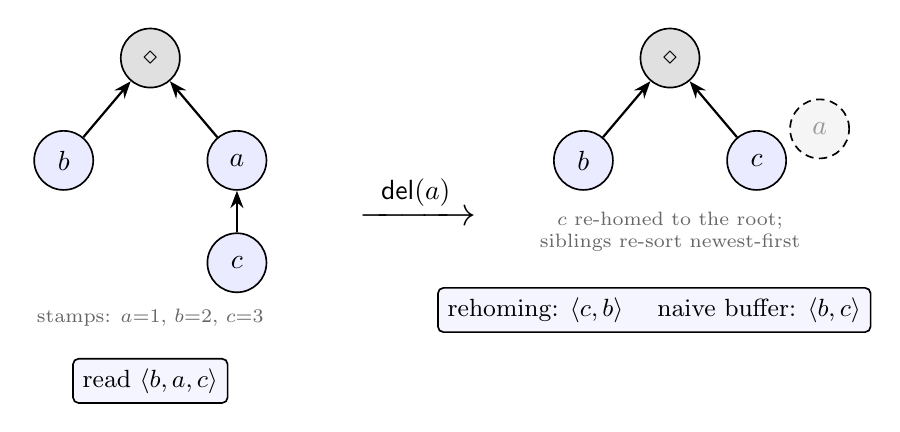
\begin{tikzpicture}
  \node[rootvtx] (r) at (0,0) {$\diamond$};
  \node[vtx] (b) at (-1.1,-1.3) {$b$};
  \node[vtx] (a) at (1.1,-1.3) {$a$};
  \node[vtx] (c) at (1.1,-2.6) {$c$};
  \draw[anc] (b) -- (r);
  \draw[anc] (a) -- (r);
  \draw[anc] (c) -- (a);
  \node[elbl] at (0,-3.3) {stamps: $a{=}1$, $b{=}2$, $c{=}3$};
  \node[stbox] at (0,-4.1) {read $\langle b, a, c\rangle$};
  \node at (3.4,-1.8) {\Large $\xrightarrow{\ \del(a)\ }$};
  \begin{scope}[shift={(6.6,0)}]
  \node[rootvtx] (r2) at (0,0) {$\diamond$};
  \node[vtx] (b2) at (-1.1,-1.3) {$b$};
  \node[deadv] (a2) at (1.9,-0.9) {$a$};
  \node[vtx] (c2) at (1.1,-1.3) {$c$};
  \draw[anc] (b2) -- (r2);
  \draw[anc] (c2) -- (r2);
  \node[elbl, align=center] at (0,-2.2)
    {$c$ re-homed to the root;\\ siblings re-sort newest-first};
  \node[stbox] at (-0.2,-3.2) {rehoming: $\langle c, b\rangle$
    \quad naive buffer: $\langle b, c\rangle$};
  \end{scope}
\end{tikzpicture}
\caption{The four-op refutation. One replica, no merge. Deleting $a$
swaps the surviving $b$ and $c$ in the rehoming RGA's read; the naive
buffer keeps their order. The embedded-chain RGA reads
$\langle b, c\rangle$ on the same trace: $c$'s immutable coordinate
still carries $a$'s chain as pure geometry, so nothing moves.}
\label{fig:refutation}
\end{figure}

\paragraph{Fused Peritext on the rehoming kernel fails at the render
(\code{fused\_delete\_reformats\_survivor}).}
The same reorder lifted to $\mathrm{char} \oplus \mathrm{boundary}$:
deleting a plain character re-homes a survivor past a mark boundary,
and an untouched character changes formatting, on one replica. This
upgraded the re-base of Peritext onto the embed kernel from
housekeeping to a correctness fix. On the embed kernel the
corresponding \emph{general} theorem holds: \code{renderIds\_del}
(axioms $\{\mathrm{propext}, \mathrm{Quot.sound}\}$): deleting a
character leaves every other character's rendered formatting bitwise
untouched, because character entries are open-set-neutral and delete
is a filter on an order-canonical state.

\paragraph{Shesha passes sequentially and fails at the merge.}
The mirror image. Shesha's single-replica reads are the naive linked
list (\code{sequential\_soundness}, kernel-clean), and it uniquely
preserves survivor order under delete among the tombstone-free designs
of its generation (\code{delete\_preserves\_survivor\_order}). Its
\emph{merge} is machine-checked non-RA-linearizable
(\code{Shesha\_Rows\_Refuted}): at an honest reachable configuration
the three-way merge splits a deleted node's children around a
concurrent sibling, producing a read that is the fold of no
delivery-respecting linearization.

\section{The two-axis separation}
\label{sec:axes}

Together the refutations witness that do-faithfulness and
merge-faithfulness are \emph{independent} axes
(Figure~\ref{fig:axes}): the rehoming family occupies
merge-yes/do-no, Shesha do-yes/merge-no, and the embedded-chain family
shows the top corner is achievable, by one design idea in both
sequence datatypes: immutable birth coordinates, so that deletion
moves nothing and the merge decides nothing.

\begin{figure}[h]
\centering
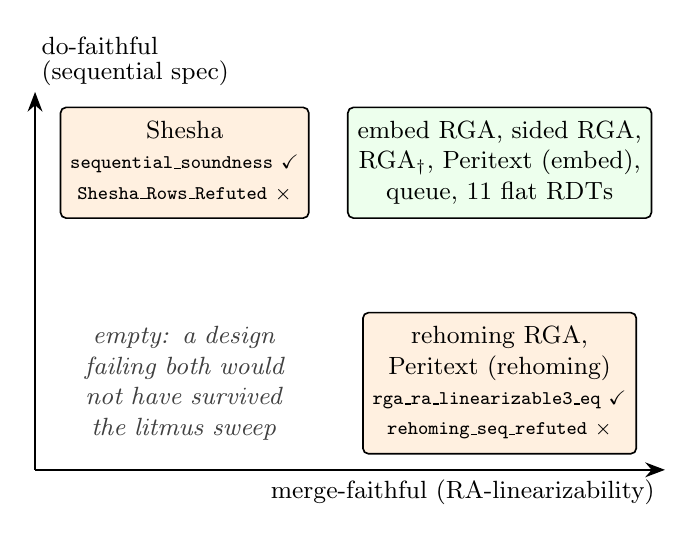
\begin{tikzpicture}[scale=1.0]
  \draw[-{Stealth[length=2.5mm]}, line width=0.9pt] (0,0) -- (8.0,0)
    node[below left, font=\small] {merge-faithful (RA-linearizability)};
  \draw[-{Stealth[length=2.5mm]}, line width=0.9pt] (0,0) -- (0,4.8)
    node[above right=-2pt, font=\small, align=left] {do-faithful\\[-2pt]
      (sequential spec)};
  \node[okbox] at (5.9,3.9)
    {\begin{tabular}{@{}c@{}}embed RGA, sided RGA,\\
      RGA$_\dagger$, Peritext (embed),\\ queue, 11 flat RDTs\end{tabular}};
  \node[badbox] at (1.9,3.9)
    {\begin{tabular}{@{}c@{}}Shesha\\
      \scriptsize\code{sequential\_soundness} $\checkmark$\\
      \scriptsize\code{Shesha\_Rows\_Refuted} $\times$\end{tabular}};
  \node[badbox] at (5.9,1.1)
    {\begin{tabular}{@{}c@{}}rehoming RGA,\\ Peritext (rehoming)\\
      \scriptsize\code{rga\_ra\_linearizable3\_eq} $\checkmark$\\
      \scriptsize\code{rehoming\_seq\_refuted} $\times$\end{tabular}};
  \node[capt, align=center, text width=3.1cm] at (1.9,1.1)
    {empty: a design failing both would not have survived the litmus
     sweep};
\end{tikzpicture}
\caption{Every placement is a named kernel theorem. The two failure
modes are orthogonal: converging to a reordering fold (bottom right)
and folding correctly into a non-linearizable merge (top left).}
\label{fig:axes}
\end{figure}

\section{What composition does not give}
\label{sec:caveat}

It is tempting to compose the guarantees: RA-linearizability says
every version is $\mathrm{fold}(\rho)$ for some delivery-respecting
$\rho$ over the event union; the campaign says folds of sequentially
honest histories equal the spec program. May one conclude that every
merged document is the naive program's output on \emph{some} ordering
of everyone's operations? \textbf{No}, and the failure is precise.

The campaign's theorems quantify over \emph{sequentially honest}
histories; an RA-linearizability witness is delivery-respecting but
need not be sequentially honest on either count. Stamp monotonicity
fails harmlessly: when the state is a function of the event set
(fold-canonicity, \code{e\_fold\_canon}), any enumeration can be
re-sorted. Applicability is the real corner
(Figure~\ref{fig:deadanchor}): in the union of two branches, an
insert's anchor may be deleted by a \emph{concurrent} operation
carrying a smaller Lamport stamp, so in stamp-sorted order the delete
precedes the insert, the anchor is dead at the insert's prefix, and
the naive buffer no-ops the splice, while the datatype (whose
coordinates travel in the op) places the element correctly. Some
interleavings of the union match the spec program and some do not.

\begin{figure}[h]
\centering
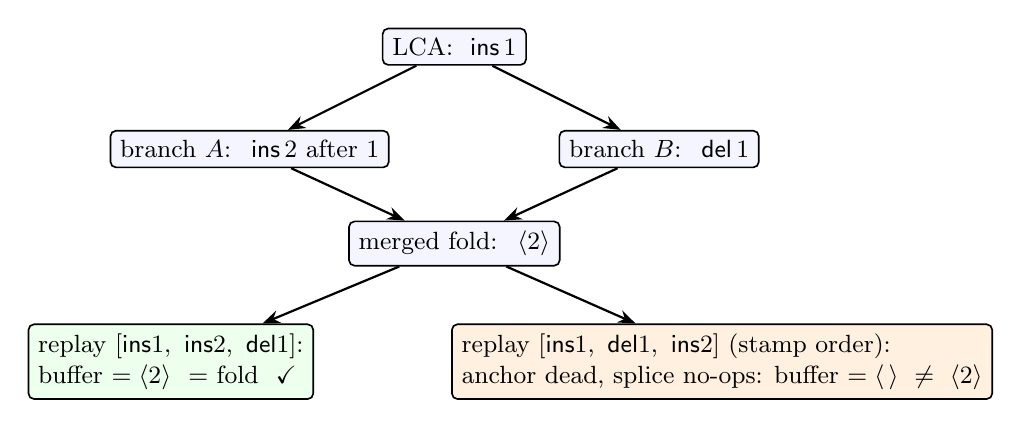
\begin{tikzpicture}
  \node[stbox] (lca) at (0,0) {LCA: \ $\ins\,1$};
  \node[stbox] (ba) at (-2.6,-1.3) {branch $A$: \ $\ins\,2$ after $1$};
  \node[stbox] (bb) at (2.6,-1.3) {branch $B$: \ $\del\,1$};
  \draw[anc] (lca) -- (ba);
  \draw[anc] (lca) -- (bb);
  \node[stbox] (m) at (0,-2.5) {merged fold: \ $\langle 2 \rangle$};
  \draw[anc] (ba) -- (m);
  \draw[anc] (bb) -- (m);
  \node[okbox, align=left] (g) at (-3.6,-4.0)
    {replay $[\ins 1,\ \ins 2,\ \del 1]$:\\
     buffer $= \langle 2\rangle$ \ $=$ fold \ $\checkmark$};
  \node[badbox, align=left] (b) at (3.4,-4.0)
    {replay $[\ins 1,\ \del 1,\ \ins 2]$ (stamp order):\\
     anchor dead, splice no-ops: buffer $= \langle\,\rangle
       \ \neq \ \langle 2 \rangle$};
  \draw[anc] (m) -- (g);
  \draw[anc] (m) -- (b);
\end{tikzpicture}
\caption{The dead-anchor corner. The merged fold keeps $2$ (OR-set
survival on immutable coordinates); whether a naive-buffer replay of
the union agrees depends on which delivery-respecting order is chosen,
and the stamp-sorted one can be wrong. This is the same corner the
sequence-CRDT trilemma names for insert-after-already-deleted-anchor.}
\label{fig:deadanchor}
\end{figure}

Whether a matching order always exists is genuinely open; it is
recorded as Open Question~\ref{oq:seqwitness} in the consolidated
list.

Independently of the question, the composition that \emph{is} sound
and kernel-checked today: every version is the datatype's fold of a
delivery-respecting enumeration (RA-linearizability); the fold is
canonical per event set (\code{e\_fold\_canon}); each replica's own
contribution obeyed the sequential spec while it was being made (this
campaign); and merge-level intent is delivered by separate, named
theorems where it holds (delete-order preservation as sublist
stability, subtree convexity as non-interleaving, read-equivalence to
the published RGA as the compaction theorem). The campaign does not
manufacture a merge-level user story; it pins the single-replica story
so that merge-level claims have something sound to stand on.

\section{The verified matrix}
\label{sec:matrix}

The anomaly-comparison matrix (task \#64,
\code{whiteboard/anomaly-matrix/}) ran six implementations and four
production libraries through 25{,}917 merges per row, every cell
backed by executed code. Its in-repo rows have since been upgraded
from machine-run to kernel-checked; the table below is the matrix's
load-bearing core with each cell a Lean identifier. External libraries
(Yjs, Automerge, Loro, list-positions) remain empirical by nature;
their rows live in the matrix report unchanged.

\begin{center}\scriptsize
\begin{tabular}{@{}lll@{}}
\toprule
design & sequential spec (do) & RA-lin (merge) \\
\midrule
embedded-chain RGA & \code{embed\_seq\_sound} &
  \code{embed\_ra\_linearizable3} \\
sided RGA (two-sided) & \code{sided\_seq\_sound} &
  \code{sided\_embed\_ra\_linearizable3} \\
published RGA$_\dagger$ & \code{rga\_seq\_read\_eq\_buffer} &
  \code{rgaWithTombstones\_ra\_lin...\_eq} \\
Peritext (embed) & \code{peritextEmbed\_seq\_sound} &
  \code{peritextEmbed\_ra\_linearizable3} \\
mergeable queue & \code{queue\_seq\_sound} &
  \code{queue\_ra\_linearizable3} \\
eleven flat RDTs & \code{*\_seq\_sound} &
  \code{*\_ra\_linearizable3\_eq} \\
\midrule
rehoming RGA & \textbf{refuted}: \code{rehoming\_seq\_refuted} &
  \code{rga\_ra\_linearizable3\_eq} \\
Peritext (rehoming) & \textbf{refuted} (render):
  \code{fused\_delete\_reformats\_surv...} &
  \code{peritext\_ra\_lin..\_eq} \\
Shesha & \code{sequential\_soundness} &
  \textbf{refuted}: \code{Shesha\_Rows\_Refuted} \\
\bottomrule
\end{tabular}
\end{center}

\noindent Every positive theorem above is kernel-clean (axioms
$\subseteq \{\mathrm{propext}, \mathrm{Classical.choice},
\mathrm{Quot.sound}\}$; the queue's and \code{renderIds\_del}'s audits
omit choice). Refutations by concrete witness follow the SPOT
convention (\code{native\_decide}, adding the compiler axioms); the
refuted \emph{statements} are quantified properties whose honesty
guards are discharged on the witness.

%======================================================================
\part{Open questions and the mechanization map}
%======================================================================

\section{Open questions}
\label{sec:open}

The consolidated list: the framework questions of the metatheory
(Part~I), the campaign's successor question (Part~III), and two
questions raised by the FugueMax arc (Part~II). One resolved question
is kept at the end in compressed form, because the later parts depend
on its correction.

\begin{openq}[Is there a rely-guarantee program logic for MRDTs?]
\label{oq:proglogic}
The framework already carries the skeleton of a verification-condition logic:
the signature-plus-conditioning is the ``program'', RA-linearizability up to
$\eqobs$ is the judgment, the eight VCs are local proof obligations, the
metatheorem is their \emph{soundness theorem}, and the product $\otimes$ with
\lean{JoinLemma3At} is a frame/composition rule (the coupling hierarchy
L0--L3 stratifying it by interaction strength, as disjoint-vs-shared
reasoning does in separation logic). The conditioning layer is specifically
\emph{rely-guarantee}: honest delivery is the \emph{rely} (an assumption on
other replicas' and clients' steps), convergence/safety up to $\eqobs$ is the
\emph{guarantee}, merges are environment steps, and the ``stable under
concurrent honest extension'' condition the safety metatheorem turns on
(\S\ref{sec:route}: the bounded counter succeeds and
BudgetCart/FWW fail on exactly it) \emph{is} the rely-guarantee stability
side-condition, arrived at independently. What is missing to make it a
program logic proper is a \emph{syntax}: a language building $\dodo$/$\merge$
from primitives (a per-replica counter cell, OR-set membership, an LWW/FWW
$\max$/$\min$ cell, a sequence node) and combinators (the product $\otimes$,
the indexed map, the payload-parametric wrap of \lean{ORSetCore}), each
carrying its local VC contribution and its join-species, such that
well-formedness entails RA-linearizability \emph{by construction} --- so that
writing an MRDT and proving it converge become one act, as separation logic
made heap-program verification syntax-directed. The \emph{semantic}
combinators already exist and are each \emph{separately} proven sound; what
is open is the grammar together with a \emph{single} soundness theorem for
the grammar (not one per combinator). This question subsumes the two
framework-theory questions below: $\cd$-derivability (\ref{oq:cd}) asks
whether the rule set is minimal, and the structure theorem asks to classify
the primitives.
\end{openq}

\begin{openq}[$\cd$-derivability]
\label{oq:cd}
Is $\cd$ derivable from VCs 1--7 (plus the unconditional delta laws where
they hold)? Specializing the merge to an LCA-blind lattice join --- the
CRDT case --- the question closes exactly: there, the corresponding
causal-delta bound is \emph{equivalent} to the Join Lemma and no strictly
weaker bridge VC exists, with both attack routes
characterized --- the positive induction is circular at two identified case
shapes, and the countermodel space is narrowed to non-atomic lattice
states (all of this mechanized, in \lean{Sal/CRDTs/Metatheory/}). The
ternary question, by contrast, is now \textbf{closed}: \lean{CDVC3} is an
\emph{independent} rule of the ternary bundle
(\lean{cdvc3\_not\_derivable\_from\_core\_delta},
\lean{Refutations/CD\_Not\_Derivable\_Ternary.lean}, kernel-clean) --- there is
a \lean{ConditionedMRDTSig} (\lean{AWSetF3}, the LCA-blind lift of the binary
inflation-separator, with a deflationary $\mathsf{rem}$) satisfying every
\lean{CoreVCs3} and \lean{DeltaVCs3} clause yet falsifying \lean{CDVC3}, so
$\mathsf{CoreVCs3} + \mathsf{DeltaVCs3} \not\Rightarrow \mathsf{CDVC3}$ (and,
via \lean{joinLemma3\_iff\_cdVC3}, $\not\Rightarrow$ the Join Lemma). The
reason ternary \emph{closes} where binary (b$''$) stays open is instructive:
\lean{CDVC3}'s $\sqsubseteq$-half demands update \emph{inflation}
($A \sqsubseteq \mathsf{update}\,A\,e$), which the binary \lean{LatticeVCsPlus}
ships as a separate axiom but the ternary \lean{DeltaVCs3} honestly omits ---
so the inflation-free delta laws cannot back \lean{CDVC3}, and a deflationary
update refutes it. The eight-VC bundle is therefore \textbf{minimal at
\lean{CDVC3}}: the causal-delta rule is a genuine independent axiom, not a
derived lemma (a load-bearing point for the rule-basis of
Open Question~\ref{oq:proglogic})
\end{openq}

\begin{openq}[structure theorem]
\label{oq:structure}
Empirically, the \emph{unconditional} delta contract holds exactly on the
group and lattice classes. Is every unconditional-$\mathsf{DeltaVCs3}$
merge a torsor-like group$\,\otimes\,$lattice combination? (The na\"ive
two-sorted umbrella $\mergeL(l,a,b) = a \boxplus (b \boxminus l)$ does
\emph{not} derive the contract uniformly, so the question is genuinely
open.)
\end{openq}

\begin{openq}[the automation layer]
The published catalogue's seventeen induction-scheme VCs were an
SMT-facing Skolemization of feasibility, aimed at the wrong target.
Design the analogous per-data-type induction scheme whose induction
implies $\cd$ and the feasible delta laws --- restoring push-button
discharge, now of VCs that actually imply RA-linearizability. The
observed uniformity of the discharges ($\sigma$-characterization by
sandwich invariant + absorber trichotomy) suggests the scheme exists.
\end{openq}

\begin{openq}[criss-cross merges and virtual LCAs]
\label{oq:crisscross}
The transition system gates Merge on the existence of an LCA
(\S\ref{sec:lca}); criss-cross configurations are reachable, and every
version in them linearizes, but their heads cannot merge --- the model
is silent exactly where git reaches for its \emph{recursive} strategy
(merge the maximal common ancestors into a virtual base, then merge with
that). The metatheory looks ready for the extension: the ternary Join
Lemma is stated over backward-closed \emph{event sets}, and
$E_1 \cap E_2$ needs no witnessing store version. What remains is a
virtual-LCA Merge rule plus one per-data-type question: do the eight VCs
imply that the recursively computed base equals
$\sigma(E_1 \cap E_2)$? For the counter this is inclusion--exclusion
once more --- exact iff the maximal common ancestors jointly cover the
intersection, itself a candidate store invariant; for the OR-set, a
pointwise Boolean check. A positive answer closes the one visible gap
between the model and practice.
\end{openq}

\begin{openq}[$\rcrel$-expressiveness: chains, LWW, and
merge-recoverability]
\label{oq:rcchain}
The catalogue's $\rcrel$ relations are all \emph{star-shaped}: the
conflicting pairs are cross-class ($\rem$/$\add$; add/checkout), so every
edge runs from a class that is never second to a class that is never
first. This is forced: the update layer's directionality law
(\lean{rc\_non\_comm\_directional}) orients every non-commuting concurrent
pair, while its companion \lean{no\_rc\_chain} forbids length-2 paths, and any orientation of a \emph{self}-conflicting
class (concurrent writes; concurrent claims of one slot) contains one. So
total-order policies --- last-writer-wins first among them --- are
inexpressible in the $\rcrel$ mechanism as constrained by the VC set.
Two questions, one of them already closed at its boundary. (i)~Would a
\emph{chain-tolerant} generalization (the concurrent arm of $\mathsf{lo}$ as a
transitive tiebreak) be sound? The semantics is coherent --- with Lamport
clocks the composite of $\mathsf{vis}$ and any timestamp- or priority-oriented
tiebreak is acyclic, and canonical states remain well-defined --- so the
restriction appears to be an artifact of the swap-flavored proof
machinery (\lean{cond\_comm\_lift} cannot bubble past two consecutive
$\rcrel$ edges), not of the theorem. The decisive experiment:
re-prove the swap VC and the causal-delta peel over a transitive
tiebreak; we expect the swap route to break and the canonical-state route
(which peels a global maximum, and a total order has one everywhere) to
survive. (ii)~What would it buy? \emph{Not} a metadata-free LWW register:
whatever the order arbitrates, the converged outcome must be produced by
$\mergeL(l,a,b)$ --- a function of three \emph{states} --- and for a
plain-value LWW two executions present identical state triples with
opposite timestamp orders, so no such function exists
(\lean{lww\_merge\_needs\_timestamps},
\lean{Refutations/LWW\_Merge\_Needs\_Timestamps.lean}, kernel-checked).
The arbitration key is forced into the state by the \emph{merge}; once
there, writes commute and $\rcrel$ is moot --- which is why every
LWW implementation stores its timestamp. What a chain-tolerant arm
\emph{could} buy: metadata-free \emph{priority} policies across three or
more op classes (outcomes state-recoverable, orientations chained). The
general principle the kill-test
isolates: $\rcrel$ is the mechanism for conflicts whose outcome is
recoverable from branch states; clique conflicts pay for their arbitration
key in state, and chains would extend $\rcrel$ only within the
recoverable class.
\end{openq}

\begin{openq}[Causal canonicity under general $\rcrel$]
\label{oq:causalcanon}
The generic safety metatheorem consumes \emph{causal} canonical
witnesses --- enumerations linearizing $\vis$ and respecting $\loE{E}$
jointly. With every concurrent pair unordered (Either), the two discharge
species of \S\ref{sec:route} suffice. Under a general $\rcrel$ the
existence of a
joint linearization is open: a cycle would need at least two
$\rcrel$-edges separated by $\vis$-paths --- a single
$\rcrel$-edge closed by a $\vis$-path contradicts concurrency via
transitivity, and a non-commuting first $\vis$-step is an absorber
killing the edge --- and \lean{no\_rc\_chain} forbids adjacent
$\rcrel$-edges but not $\vis$-separated ones. \lean{CausalCanonical} is therefore a hypothesis with two discharge
lemmas rather than a theorem. The budget cart (\lean{BudgetCart},
\lean{MRDT\_Instances/BudgetCart/}) has now \emph{forced} the question ---
and widened it: its convergence discharges along the OR-set route, but the
ungated safety obligation \lean{SafetyStepOn} is \emph{false} for it, by a
two-event refutation --- \lean{CausalFold} pins only $\vis$-respect, and
the fold of a causal past containing a concurrent same-item
$\mathsf{add}/\mathsf{rem}$ pair is enumeration-dependent (the orders
disagree exactly where add-wins should arbitrate). So for
$\rcrel$-nontrivial datatypes the \emph{honesty fold} needs
$\rcrel$-orientation too: the right notion is folds along jointly
$\vis$- and $\loE{E}$-respecting enumerations, for both the version
witnesses (\lean{CausalCanonical}) and the causal-past folds
(\lean{CausalFold}). The cart's safety theorem is delivered gated
(\lean{bcart\_version\_inv\_gated}, with the missing transfer named
explicitly as \lean{BCartSpendMono}); closing the gate is this question.
\end{openq}

\begin{openq}[Does conditioning compose? --- convergence: yes, now a theorem]
\label{oq:compose}
The catalogue is built one data type at a time; practice builds data types
from data types --- the canonical case is the key-value map whose values are
themselves MRDTs (the certified-MRDT line's own composite). The factored
framework suggests composition should happen at the \lean{JoinLemma3At}
boundary --- the map combinator would consume each value's per-configuration
join, whatever species produced it, so a map of \emph{queues} composes as
readily as a map of counters --- with a small once-only kit: folds and
configurations project per key, cross-key pairs commute so $\loE{E}$
localizes, and per-key joins re-interleave. Conjecturally the coupling
strength stratifies what survives composition: payload parametricity (free),
the indexed product = the grow-only-keys map (a theorem to prove), read
coupling --- one layer's $\app$ reads another's state, as in a budgeted
cart --- (convergence composes; safety needs a monotone-transfer lemma),
uniform coupling --- key \emph{removal}, reaching into the value layer the
same way for every value type (one generic obligation: a reset element and
a $\mathsf{remove} \parallel v$-op policy) --- and ad-hoc effect coupling
(rich-text marks anchored in a sequence), where nothing is expected to
compose automatically. The convergence half is now mechanized
(\lean{Metatheory/Product.lean}): the binary heterogeneous product
$D_1 \otimes D_2$ composes at exactly the \lean{JoinLemma3At} boundary ---
cross-component pairs commute definitionally, so $\loE{E}$ has \emph{no}
mixed edges and the glued join witness is a plain concatenation
$\iota_1\rho^1 \mathbin{+\!\!+} \iota_2\rho^2$
(\lean{joinLemma3At\_prod}; composite metatheorem
\lean{prod\_ra\_linearizable3\_of\_honest\_reach}, axioms \lean{propext},
\lean{Quot.sound}; consumability demo: a queue $\otimes$ counter capstone
with zero bespoke proof, \lean{MRDT\_Instances/ProductDemo/}). Two
boundary findings from the pen-and-paper pass
(\lean{Development/COMPOSITION\_PENPAPER.md}): \emph{reachability does
not project} (a second-component apply is a version-duplicating stutter
for the first's projection), so finished capstones never compose ---
only per-configuration certificates do, which retroactively forces the
factored interface of \S\ref{sec:route}; and \emph{two-sided causal-witness
re-interleaving is refuted} (a realizable four-event cross-$\vis$ cycle),
with the sound repair --- pin one side, re-sort the other --- covering
products with at most one $\rcrel$-nontrivial component. The safety and $\eqobs$ kits are also
mechanized: honesty, \lean{SafetyStep}, and \emph{one-sided} causal
witnesses compose (\lean{Metatheory/Product\_Safety.lean}: the
pinned-extension lemma, \lean{safetyStepOn\_prod},
\lean{causalCanonical\_prod\_of\_one\_sided}, composite
\lean{prod\_version\_inv\_on\_of\_one\_sided}), and the eq-quotient layer
lifts at the pragmatic cut $\eqobs_2 = {=}$
(\lean{Metatheory/ProductEq.lean}: every \lean{GenericEqQuotient}
obligation componentwise, \lean{eqJoinLemma3C\_H\_prod} glued by
concatenation with no congruence chasing, capstone
\lean{prod\_ra\_linearizable\_up\_to\_eq\_H} --- one quotiented component,
one flat, exactly the Peritext shape, with the quotiented side's
reachability supplies as premises per the memo's cost-center analysis).
Still open: the general $\eqobs_1 \times \eqobs_2$ lift (no new ideas,
double the plumbing --- deferred until a second quotiented component
exists), the indexed (map-of-MRDTs) generalization, and the L2.5/L3
coupling boundaries, where composition \emph{breaking} is expected to be
as informative as where it holds.
\end{openq}

\begin{openq}[the sequential witness at merges]
\label{oq:seqwitness}
On every honestly reachable configuration of the embedded-chain RGA,
does the event union admit a delivery-respecting enumeration that is
also sequentially honest, so that the merged read is the naive
buffer's output on it? Caution from adjacent territory: for the
rehoming design the analogous ``order dependency edges first''
discipline is refuted (the \code{DepComp} refutation, via rehoming
non-transitivity). The embed's immutable coordinates remove that
refutation's mechanism, but no proof exists in either direction.
\end{openq}

\begin{openq}[the display-to-traversal theory, and the first mechanized
maximal non-interleaving]
\label{oq:traversal}
The FugueMax arc (\S\ref{sec:mechanization}) formalized the
Weidner--Kleppmann maximal-non-interleaving Definition~4 over reachable
configurations, refuted it for the Fugue-with-recency policy (the
paper's own Fugue-vs-FugueMax separation, machine-checked), and proved
its condition (3) for the FugueMax kernel variant
(\lean{fuguemax\_same\_origin\_low\_first}). What remains of the full
Theorem~9 is the display-to-traversal theory (task \#88): relating the
kernel's displayed order to the tree traversal the definition
quantifies over. Completing it would yield the first fully mechanized
maximal non-interleaving theorem for a sequence datatype.
\end{openq}

\begin{openq}[the retention lower bound for tombstone-free maximal
non-interleaving]
\label{oq:retention}
The FugueMax kernel variant realizes its sibling order by embedding the
mint-time successor's key into contested R-entries, at
$\Theta(|\text{origin key}|)$ coordinate cost where plain Fugue pays
zero (\S\ref{sec:mechanization}). Is that retention a lower bound: must
any tombstone-free design achieving maximal non-interleaving carry the
right origin's ordering information in its keys? The question has a
Myhill--Nerode shape (task \#89): distinguish states that demand
different verdicts, and count what any key scheme must remember. It is
the entropy law of \S\ref{sec:encoding} meeting the ordering intent.
\end{openq}

\paragraph{Resolved: the self-referential-spec limit.}
RA-linearizability certifies that a version's state is the fold of some
delivery-respecting linearization of its events: convergence to the
datatype's \emph{own} $\dodo$-fold, with that fold as the reference. It
says nothing about whether the fold's single-replica semantics is the
intended one; a defect in $\dodo$ appears identically in the concurrent
state and its fold, and is certified as agreement. Independent
\emph{intent} specifications are therefore a separate obligation, not a
corollary of convergence. The question was resolved systematically by
the sequential-specification campaign (Part~III), which supplies the
independent specification for every production RDT; its refutations
also correct the earlier reading of the sharpest instance. The survivor
reorder exhibited by the campaign's four-op trace
(\S\ref{sec:refuted}) is not intrinsic to tombstone-freedom, it is
intrinsic to rehoming: the embedded-chain RGA is tombstone-free,
satisfies the sequential list specification in the strongest form
(\lean{embed\_seq\_sound}: the canonical state is the naive buffer,
record for record), and preserves delete order
(\lean{eUpdate\_del\_sublist}). The successor question is Open
Question~\ref{oq:seqwitness}.

\section{Mechanization map}
\label{sec:mech}

Everything above is mechanized in Lean~4 (Mathlib; axioms:
\lean{propext}, \lean{Classical.choice}, \lean{Quot.sound}; no
\lean{sorryAx} anywhere in the cited chains; refutations by concrete
witness follow the SPOT convention, \lean{native\_decide} adding the
compiler axioms) in the Sal repository. Files are relative to
\lean{Sal/ConditionedMRDTs/} unless they carry an explicit
\lean{Sal/} prefix.

\begin{center}
\footnotesize
\resizebox{0.95\textwidth}{!}{%
\begin{tabular}{@{}lll@{}}
\toprule
Artifact & Lean & File \\
\midrule
\multicolumn{3}{@{}l}{\emph{Part I: framework and metatheorems}} \\
signature, ternary $\mathsf{lo}$ & \lean{MRDTSig}, \lean{ConditionedMRDTSig} & \lean{Framework/MRDTSig.lean} \\
store, DAG, transitions & \lean{Configuration}, \lean{Step3} & \lean{Framework/ExecutionModel.lean}, \lean{Metatheory/LCA\_Lemma.lean} \\
Lemma~\ref{lem:lca} & \lean{lca\_events\_of\_storeInv} & \lean{Metatheory/LCA\_Lemma.lean} \\
$\sigma$/$\loE{E}$ layer (merge-independent) & \lean{UpdateVCs}, \lean{IsCanonicalState} & \lean{Framework/Sigma\_LoOn3.lean} \\
the eight VCs & $\co$, $\fd$, $\cd$ & \lean{Framework/VC\_Set.lean} \\
Theorem~\ref{thm:main} + bridges & \lean{ra\_linearizable\_of\_core\_}\lean{feasible\_cd3} & \lean{Metatheory/Adequacy.lean} \\
defeater vs.\ \textsc{2-OP} (\S\ref{sec:defeater}) & \lean{no\_inter\_lca\_2op\_rem\_peel\_of\_defeater} & \lean{Refutations/InterLca2op\_Defeater\_Arbiter.lean} \\
closure-indexed contract (\S\ref{sec:adequacy}) & \lean{JoinLemma3C}, \lean{no\_proper\_back\_block} & \lean{Metatheory/JoinLemma3C.lean} \\
closure-indexed adequacy + instances & \lean{ra\_linearizable3\_of\_joinC}, \lean{ConditionedContract} & \lean{Metatheory/ConditionedContract.lean} \\
all 9 flat discharges via the contract & \lean{$\ast$\_adequate\_viaContract} (9) & \lean{Development/AllMRDTs\_viaContract.lean} \\
per-configuration join hook & \lean{JoinLemma3At}, \lean{goodConfig3\_merge\_at} & \lean{Framework/VC\_Set.lean}, \lean{Metatheory/Adequacy.lean} \\
honest-reachability metatheorem & \lean{HonestReach}, \lean{ra\_linearizable3\_of\_honest\_reach} & \lean{Metatheory/HonestReach.lean} \\
generic honesty shape & \lean{GenHonest}, \lean{AppHonest} & \lean{Metatheory/GenHonest.lean} \\
witness-class join lemmas & \lean{JoinLemma3AtW} & \lean{Metatheory/WitnessClass.lean} \\
generic safety (causal witness) & \lean{SafetyStep}, \lean{version\_inv\_of\_causal\_canonical} & \lean{Metatheory/GenericSafety.lean} \\
escrow metatheorem & \lean{Measured}, \lean{escrow\_version\_inv} & \lean{Metatheory/EscrowSafety.lean} \\
product composition (raw kit) & \lean{joinLemma3At\_prod}, \lean{prod\_ra\_linearizable3\_of\_honest\_reach} & \lean{Metatheory/Product.lean} \\
product safety kit & \lean{safetyStepOn\_prod}, \lean{prod\_version\_inv\_on\_of\_one\_sided} & \lean{Metatheory/Product\_Safety.lean} \\
product $\eqobs$-lift & \lean{eqJoinLemma3C\_H\_prod}, \lean{prod\_ra\_linearizable\_up\_to\_eq\_H} & \lean{Metatheory/ProductEq.lean} \\
observational quotient $D \mapsto D_\approx$ & \lean{QSig}, \lean{qapplicable} & \lean{Metatheory/GenericEqQuotient$\ast$.lean} \\
canonical-witness layer, raw-$\approx$ target & \lean{IsRALinearizable3Eq}, \lean{RA\_linearizable\_up\_to\_eq\_H} & \lean{Metatheory/GoodConfig3H.lean} \\
flat collapse of the framework & \lean{eqJoinH\_of\_joinC}, \lean{flat\_ra\_linearizable3\_eq} & \lean{Metatheory/FlatGeneric\_Bridge.lean} \\
LWW merge needs timestamps (OQ~\ref{oq:rcchain}) & \lean{lww\_merge\_needs\_timestamps} & \lean{Refutations/LWW\_Merge\_Needs\_Timestamps.lean} \\
$\cd$ independent of core+delta (OQ~\ref{oq:cd}) & \lean{cdvc3\_not\_derivable\_from\_core\_delta} & \lean{Refutations/CD\_Not\_Derivable\_Ternary.lean} \\
impossibility kill-tests & --- & \lean{Refutations/Impossibility.lean} \\
findings journal & --- & \lean{Development/MRDT\_METATHEORY\_DRAFT.md} \\
\midrule
\multicolumn{3}{@{}l}{\emph{Part I: instances (Table~\ref{tab:catalog})}} \\
catalogue instance theorems & all instance theorems & \lean{MRDT\_Instances/} (one directory per RDT) \\
the flat instances, generically & \lean{$\ast$\_ra\_linearizable3\_eq} (11) & \lean{MRDT\_Instances/} (per-RDT) \\
bounded-counter safety & \lean{bc\_version\_inv}, \lean{bc\_value\_nonneg} & \lean{MRDT\_Instances/BoundedCounter/} \\
mergeable queue (direct join) & \lean{q\_join\_at}, \lean{queue\_ra\_linearizable3} & \lean{MRDT\_Instances/MergeableQueue/} \\
FWW register (payload arbitration) & \lean{fww\_version\_min} & \lean{MRDT\_Instances/FWWRegister/} \\
BudgetCart (gated safety) & \lean{BCart\_ra\_linearizable3\_eq}, \lean{bcart\_version\_inv\_gated} & \lean{MRDT\_Instances/BudgetCart/} \\
\midrule
\multicolumn{3}{@{}l}{\emph{Part II: the embedded-chain family}} \\
model-layer kernel & \lean{rc\_non\_comm'}, \lean{display\_iff\_chainBefore}, \lean{subtree\_convex} & \lean{Sal/MRDTs/RGA\_Embed/} \\
embedded-chain RGA (queue route) & \lean{embed\_ra\_linearizable3}, \lean{e\_fold\_canon} & \lean{MRDT\_Instances/EmbedRGA/} \\
Elias-$\delta$ inheritance corollary & (capstone at the $\delta$-flip) & \lean{MRDT\_Instances/EmbedRGA/EmbedRGA\_EliasDelta.lean} \\
compaction theorem & \lean{rga\_read\_eq\_embed\_read} & \lean{MRDT\_Instances/EmbedRGA/EmbedRGA\_ReadEquiv.lean} \\
compaction order core & \lean{visible\_lt} $=$ chain-lex & \lean{Sal/MRDTs/RGA\_Embed/RGA\_Embed\_ReadEquiv.lean} \\
sided chain-lex kernel & \lean{sdisplay\_iff\_schainBefore}, \lean{schainBefore\_liftR} & \lean{Sal/MRDTs/RGA\_Embed/Sided\_ChainLex.lean} \\
sided RGA + per-policy intent & \lean{sided\_embed\_ra\_linearizable3}, \lean{sFold\_liftOp} & \lean{MRDT\_Instances/SidedRGA/} \\
Fugue/FugueMax vs.\ W--K Def.~4 & \lean{fugue\_not\_maximally\_noninterleaving}, \lean{fuguemax\_same\_origin\_low\_first} & \lean{MRDT\_Instances/SidedRGA/}, \lean{Sal/MRDTs/RGA\_Embed/SidedMax\_ChainLex.lean} \\
Peritext on the embed kernel & \lean{peritextEmbed\_ra\_linearizable3}, \lean{renderIds\_del} & \lean{MRDT\_Instances/Peritext\_Embed/} \\
\midrule
\multicolumn{3}{@{}l}{\emph{Part III: the sequential-specification campaign}} \\
tier 1: eleven flat RDTs & \lean{$\ast$\_seq\_sound} (per RDT) & \lean{MRDT\_Instances/SeqSpec\_Flat.lean} \\
tier 2: mergeable queue & \lean{queue\_seq\_sound} & \lean{MRDT\_Instances/MergeableQueue/MergeableQueue\_SeqSpec.lean} \\
tier 3: embedded-chain RGA & \lean{embed\_seq\_sound} & \lean{MRDT\_Instances/EmbedRGA/EmbedRGA\_SeqSpec.lean} \\
tier 3, two-sided: sided RGA & \lean{sided\_seq\_sound} & \lean{MRDT\_Instances/SidedRGA/SidedRGA\_SeqSpec.lean} \\
tier 3 corollary: RGA$_\dagger$ & \lean{rga\_seq\_read\_eq\_buffer} & \lean{MRDT\_Instances/EmbedRGA/EmbedRGA\_SeqSpec\_RGA.lean} (standalone) \\
tier 4: fused Peritext & \lean{peritextEmbed\_seq\_sound} & \lean{MRDT\_Instances/Peritext\_Embed/PeritextEmbed\_SeqSpec.lean} \\
render fix theorem & \lean{renderIds\_del} & \lean{MRDT\_Instances/Peritext\_Embed/PeritextEmbed.lean} \\
negative: rehoming RGA & \lean{rehoming\_seq\_refuted} & \lean{MRDT\_Instances/RGA\_Rehoming/RGA\_SeqSpec\_Refuted.lean} \\
negative: rehoming Peritext & \lean{fused\_delete\_reformats\_survivor} & \lean{MRDT\_Instances/Peritext\_Rehoming/Peritext\_Read.lean} \S10 \\
negative: Shesha merge & \lean{Shesha\_Rows\_Refuted} & \lean{MRDT\_Instances/Shesha/Shesha\_Rows\_Refuted.lean} \\
\bottomrule
\end{tabular}}
\end{center}

The update-side layer ($\loE{E}$, convergence, $\sigma$) is
merge-independent --- it is stated over the update signature
$\langle \Sigma, \Sinit, \mathsf{do}, \rcrel\rangle$ alone --- and
is shared with the binary
(CRDT) specialization of the theory; in the repository it lives in
\lean{Sal/CRDTs/Metatheory/}, the directory that also holds the binary
exactness results quoted in Open Question~\ref{oq:cd}. The production
data types of Table~\ref{tab:catalog} are
mirrored faithfully from \lean{Sal/MRDTs/}$\ast$ (encoding deviations
documented per instance); their original 24-VC discharges are untouched.

The foundations live under \lean{Framework/}, the metatheorems under
\lean{Metatheory/}, the machine-checked negative results under
\lean{Refutations/}, and the per-RDT conditioned instances under
\lean{MRDT\_Instances/}; findings journals and superseded
routes remain under \lean{Development/}, which nothing imports. Each cited theorem is kernel-checked
with axioms in $\{\lean{propext},
\lean{Classical.choice}, \lean{Quot.sound}\}$ (no \lean{sorryAx}). They
import one linearization file carrying two unrelated \lean{sorry}s that the
cited theorems do not transitively depend on; \lean{Development/}%
\lean{CONDITIONED\_METATHEORY\_PLAN.md} is their roadmap.

\end{document}
